\documentclass[12pt]{article}

\usepackage[a4paper,width=160mm,top=20mm,bottom=20mm,bindingoffset=6mm]{geometry}
\usepackage[utf8]{inputenc}
\usepackage[italian]{babel}
\usepackage[OT1]{fontenc}
\usepackage{graphicx}
\usepackage{float}
\usepackage{fancyhdr}
\usepackage{xcolor}
\usepackage{mathtools}
\usepackage{amsmath}
\usepackage{amssymb}
\usepackage{tikz}
\usepackage{imakeidx}
\usepackage{textcomp}
\usepackage{pifont}
\usepackage{polynom}
\usepackage{algorithm}
\usepackage{algpseudocode}
\usepackage{mathtools}
\usepackage[colorlinks=true,linkcolor=black,anchorcolor=black,citecolor=black,filecolor=black,menucolor=black,runcolor=black,urlcolor=black]{hyperref}
\usepackage{cancel}
\usepackage{pgfplots}
\usepackage{caption}
\usepackage{tabularx}
\usepackage{comment}
\usepackage{float}
\usepackage{bm}



\begin{document}
\bibliographystyle{plain}
    \pagestyle{fancy}
    \everymath{\displaystyle}
    \sffamily
    \begin{figure}
        \centering
        
\includegraphics[scale=0.1]{images/uniba-logo.png}
        \caption*{Università degli Studi di Bari Aldo Moro}
    \end{figure}
    
    \title{Relazione tecnica Sustainability of RecSys}
    \author{Emanuele Fontana}
    \date{Tirocinio tesi triennale in Informatica\\Anno accademico 2023/2024}
    \maketitle
    \tableofcontents\newpage

    \section{Sostenibilità}

\subsection{Introduzione alla sostenibilità}

La sostenibilità è un concetto che si è diffuso negli ultimi anni, in particolare a partire dagli anni '80, e che ha assunto un ruolo sempre più importante nella società contemporanea. La sostenibilità è un concetto complesso e multidimensionale, che riguarda diversi aspetti della vita umana e dell'ambiente in cui viviamo. In generale, la sostenibilità si riferisce alla capacità di soddisfare i bisogni delle generazioni presenti senza compromettere la capacità delle generazioni future di soddisfare i propri bisogni. Questo significa che la sostenibilità riguarda la gestione responsabile delle risorse naturali, la tutela dell'ambiente, la promozione dello sviluppo economico e sociale, e la garanzia di un futuro migliore per tutti.
Un'esempio concreto di impegno per la sostenibilità è l' Agenda 2030 per lo Sviluppo Sostenibile, adottata dalle Nazioni Unite nel 2015. L'Agenda 2030 è un piano d'azione globale che contiene 17 Obiettivi di Sviluppo Sostenibile (SDGs) e 169 obiettivi specifici, che coprono una vasta gamma di temi, tra cui la povertà, la fame, la salute, l'istruzione, l'uguaglianza di genere, l'acqua, l'energia, il clima, l'ambiente, la pace e la giustizia. L'obiettivo dell'Agenda 2030 è quello di promuovere uno sviluppo sostenibile che sia equo, inclusivo e rispettoso dell'ambiente, e di garantire che nessuno venga lasciato indietro.

\noindent In ambito di Intelligence Artificiale, la sostenibilità è un tema di grande rilevanza, in quanto l'uso di tecnologie avanzate come l'AI può avere un impatto significativo sull'ambiente e sulla società. Ad esempio, l'AI richiede una grande quantità di risorse energetiche per funzionare, e può avere un impatto negativo sull'ambiente se non viene utilizzata in modo responsabile. Inoltre, l'AI può avere effetti sociali indesiderati, come la discriminazione e l'esclusione di determinati gruppi di persone. Per questo motivo, è importante che lo sviluppo e l'uso dell'AI siano guidati dai principi della sostenibilità, al fine di garantire che l'AI contribuisca a uno sviluppo sostenibile e equo per tutti.
Possiamo distingure due tipi di AI sostenibile \cite{sostenibilita}: \textit{Sustainability of AI} e \textit{AI for Sustainability}. Il primo ramo ha come obiettivo quello di quello di misurare la sostenibilità dello sviluppo e dell'uso di modelli AI, ad esempio misurando la \textit{carbon footprint} e l'energia usata per addestrare un modello. Il secondo ramo, invece, si occupa di utilizzare l'AI per affrontare le sfide della sostenibilità, ad esempio sviluppando modelli per la previsione del cambiamento climatico o per la gestione delle risorse naturali.


\subsection{Sostenibilità ambientale}
La sostenibilità ambientale è uno degli aspetti più importanti della sostenibilità, in quanto l'ambiente è la base su cui si fonda la vita umana e la prosperità economica. La sostenibilità ambientale riguarda la gestione responsabile delle risorse naturali, la tutela dell'ambiente e la prevenzione dell'inquinamento e del degrado ambientale. La sostenibilità ambientale si basa su principi come il rispetto per la natura, la conservazione della biodiversità, la riduzione delle emissioni di gas serra e la promozione di energie rinnovabili e pulite. La sostenibilità ambientale è fondamentale per garantire un futuro sostenibile per tutti, e per preservare il pianeta per le generazioni future.


\subsection{Green AI}

In ambito di Intelligence Artificiale, la sostenibilità è un tema di grande rilevanza, in quanto l'uso di tecnologie avanzate come l'AI può avere un impatto significativo sull'ambiente e sulla società. Ad esempio, l'AI richiede una grande quantità di risorse energetiche per funzionare, e può avere un impatto negativo sull'ambiente se non viene utilizzata in modo responsabile. Inoltre, l'AI può avere effetti sociali indesiderati, come la discriminazione e l'esclusione di determinati gruppi di persone. Per questo motivo, è importante che lo sviluppo e l'uso dell'AI siano guidati dai principi della sostenibilità, al fine di garantire che l'AI contribuisca a uno sviluppo sostenibile e equo per tutti.
Possiamo distingure due tipi di AI sostenibile \cite{sostenibilita}: \textit{Sustainability of AI} e \textit{AI for Sustainability}. Il primo ramo ha come obiettivo quello di quello di misurare la sostenibilità dello sviluppo e dell'uso di modelli AI, ad esempio misurando la \textit{carbon footprint} e l'energia usata per addestrare un modello. Il secondo ramo, invece, si occupa di utilizzare l'AI per affrontare le sfide della sostenibilità, ad esempio sviluppando modelli per la previsione del cambiamento climatico o per la gestione delle risorse naturali.

\noindent Con il termine \textcolor{green}{Green AI} \cite{GreenAI} ci si riferisce alla ricerca e allo sviluppo di modelli di intelligenza artificiale che tengano conto del costo computazione, delle risorse utilizzate e dell'impatto ambientale. Questa si differenzia dalla \textcolor{red}{Red AI} il cui obiettivo è quello di ottenere modelli sempre più complessi e performanti, senza tenere conto delle risorse utilizzate e dell'impatto ambientale. Dunque la Green AI promuove un approcio in cui si tiene conto del trade-off tra performance e efficienza, cercando di ottenere modelli che siano performanti ma che allo stesso tempo siano sostenibili e rispettosi dell'ambiente.
La Green AI tieni dunque conto dell' \textbf{Efficienza energetica}: i modelli di AI devono essere progettati in modo da utilizzare meno risorse energetiche possibili, ad esempio riducendo il numero di parametri, la complessità del modello e il numero di operazioni computazionali.
Alcuni fattori da tenere in considerazione sono:
\begin{itemize}
    \item \textbf{Hardware}: l'hardware utilizzato per addestrare e eseguire i modelli di AI può avere un impatto significativo sull'efficienza energetica. Ad esempio, l'uso di hardware specializzato come le GPU può ridurre il tempo di addestramento e il consumo energetico rispetto all'uso di CPU tradizionali.
    \item \textbf{Algoritmi}: la scelta degli algoritmi di AI può influenzare l'efficienza energetica dei modelli. Alcuni algoritmi sono più efficienti di altri in termini di consumo energetico e risorse computazionali, e possono essere preferiti per ridurre l'impatto ambientale.
    \item \textbf{Parametri}: il numero di parametri di un modello di AI può influenzare il consumo energetico e le risorse computazionali richieste per addestrare e eseguire il modello. Ridurre il numero di parametri può migliorare l'efficienza energetica del modello.
    \item \textbf{Emissioni di gas serra}: le emissioni di gas serra prodotte durante l'addestramento e l'esecuzione dei modelli di AI possono contribuire al cambiamento climatico e all'inquinamento atmosferico. Ridurre le emissioni di gas serra è un obiettivo importante per la Green AI.
\end{itemize}



    \newpage
    \begin{frame}{RecSys - Introduzione}
\begin{itemize}
\item Software che suggerisce all'utente elementi di interesse basandosi sulle preferenze e i comportamenti passati.
    \item Migliorano l'esperienza utente
    \item Utilizzano AI
\end{itemize}
\begin{figure}[h!]
    \centering
    \begin{minipage}{0.15\textwidth}
        \centering
        
\includegraphics[width=\textwidth]{images/netflix.png}
    \end{minipage}\hfill
    \begin{minipage}{0.15\textwidth}
        \centering
        
\includegraphics[width=\textwidth]{images/amazon.png}
    \end{minipage}\hfill
    \begin{minipage}{0.15\textwidth}
        \centering
        
\includegraphics[width=\textwidth]{images/spotify.png}
    \end{minipage}\hfill
    \begin{minipage}{0.15\textwidth}
        \centering
        
\includegraphics[width=\textwidth]{images/tiktok.png}
    \end{minipage}
    \caption{Alcuni famose piattaforme che utilizzano sistemi di raccomandazione}
\end{figure}
\end{frame}

\begin{frame}{RecSys - Tipologie}
\begin{itemize}
    \item \textbf{Collaborative Filtering}: basato sulle preferenze degli utenti (user-user, item-item)
    \item \textbf{Content-based Filtering}: basato sul contenuto degli item.
    \item \textbf{Knowledge-based}: basato su conoscenza esterna (es. knowledge graph)
    \item \textbf{Hybrid}: combinazione delle precedenti.
\end{itemize}
\end{frame}

    \newpage
    \section{Design esperimenti}



\noindent Il lavoro svolto consiste nel: 
\begin{itemize}
    \item valutare e prevedere l'impatto ambientale di un sistema di raccomandazione (RecSys) in base alla sua sostenibilità
    \item cercare una soluzione per ridurre l'impatto ambientale di un RecSys senza però perdere di performance in modo significativo.
\end{itemize}

\noindent Nella prima parte dunque sono stati effettuati ulteriori esperimenti per valutare l'impatto ambientale di diversi modelli di raccomandazione su diversi dataset. Questi dati sono stati utilizzati per addestrare un modello di regressione che permette di prevedere le emissioni prodotte da un modello di raccomandazione in base a diversi parametri.


\noindent Nella seconda parte, invece, ci si è concentrati su come ridurre l'impatto ambientale di un RecSys senza però perdere di performance. In particolare, si è cercato di capire se fosse possibile ridurre le emissioni prodotte da un modello di raccomandazione senza però perdere di performance in modo significativo.



\noindent Per quanto riguarda la valutazione, mediante la libreria CodeCarbon\footnote{\href{http://codecarbon.io}{CodeCarbon}}{} è stato possibile misurare le emissioni prodotte dalla macchina durante l'addestramento con parametri di default per un dato modello dato un dataset. 
In questo ambito  Spillo et al.\cite{spillo2023towards} mostrano come spesso algoritmi più semplici riescono ad avere delle performance molto simili a modelli più complessi, ma con un impatto ambientale decisamente minore.

\section{Situazione Attuale}


\subsection{Introduzione}

\noindent Per quanto riguarda la previsione questo prima parte del documento si propone di presentare lo stato attuale del lavoro svolto in questo ambito.

\begin{figure}[H]
    \centering
    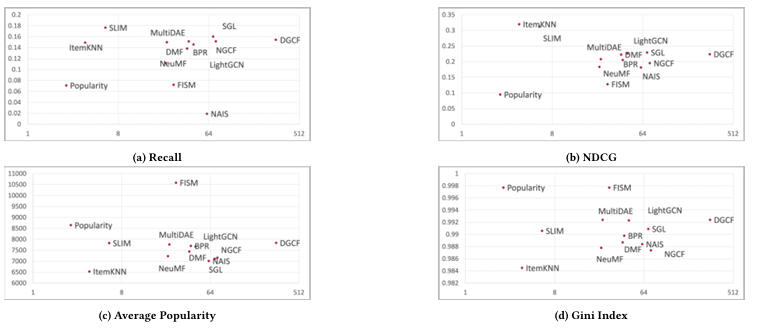
\includegraphics[scale=0.75]{images/risultati-valutazione.png}
    \caption{Trade-off tra emissioni e performance con dataset Mind}


\end{figure}



\begin{figure}[H]
    \centering
    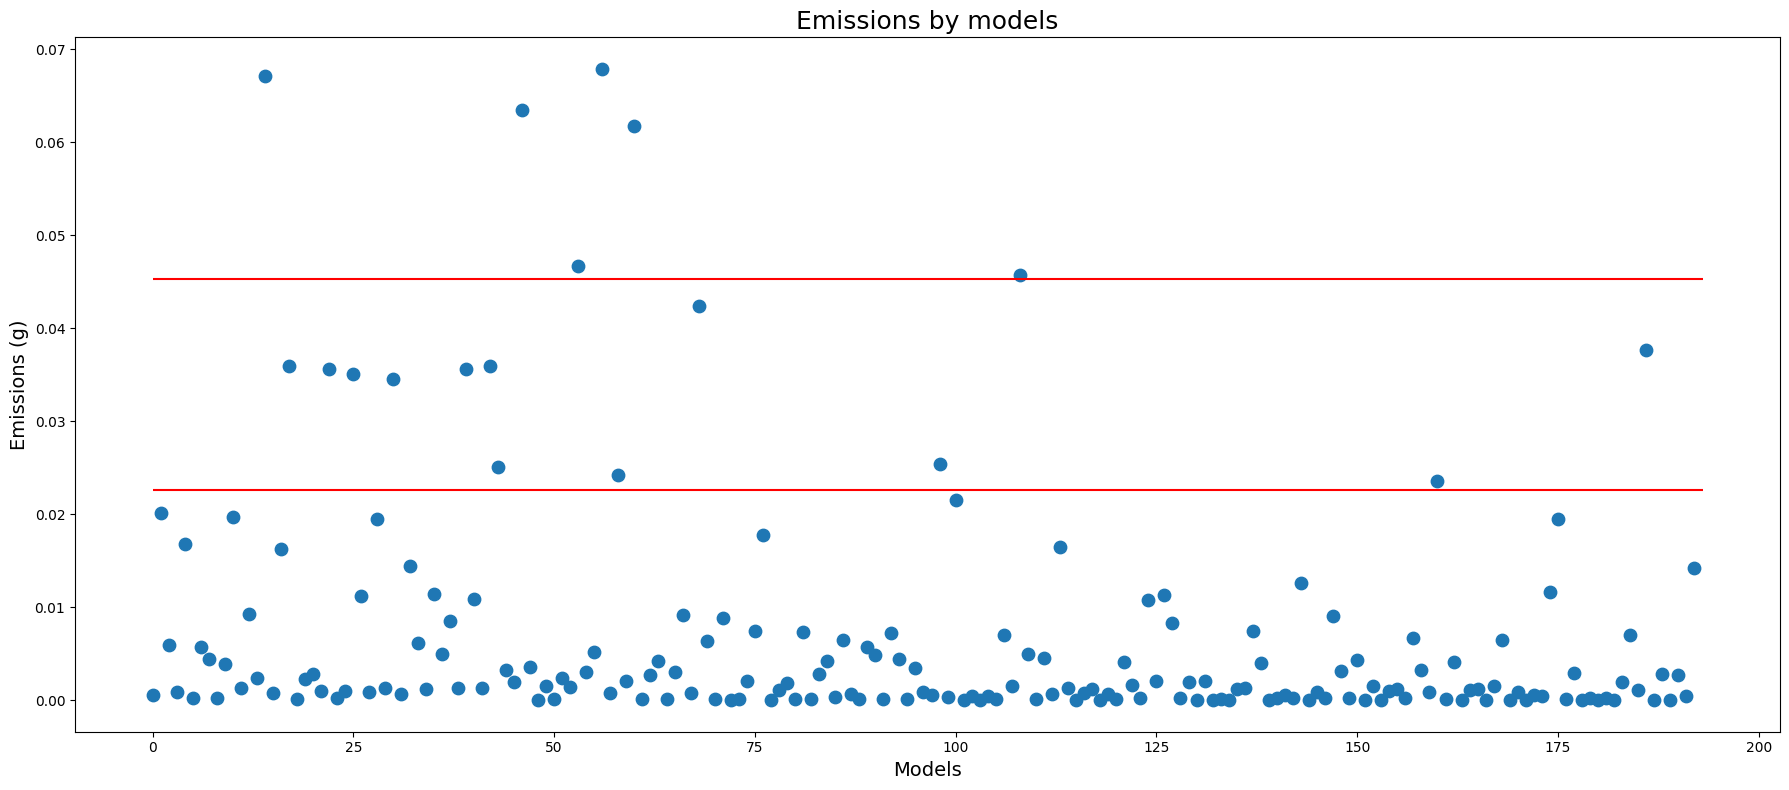
\includegraphics[scale=0.25]{images/situazione-attuale.png}
    \caption{Emissioni prodotte dai vari modelli}
\end{figure}

\noindent L'esperimento è stato condotto su dataset presenti all'interno della libreria python RecBole\footnote{\href{http://recbole.io}{RecBole}}{}, una libreria open-source che offre un'implementazione di modelli di raccomandazione. I dataset utilizzati per l'addestramento dei modelli sono:
\begin{itemize}
    \item \textbf{MovieLens-1M}\footnote{\href{https://github.com/RUCAIBox/RecSysDatasets/blob/master/conversion_tools/usage/MovieLens.md}{Dataset MovieLens}}{}
    \item \textbf{Amazon\_Book\_60core\_kg} \footnote{\href{https://github.com/RUCAIBox/RecSysDatasets/blob/master/conversion_tools/usage/Amazon-book-KG.md}{Dataset Amazon\_Book\_60core\_kg}}{}
    \item \textbf{Mind}\footnote{\href{https://github.com/RUCAIBox/RecSysDatasets/blob/master/conversion_tools/usage/MIND.md}{Dataset MIND}}{}
\end{itemize}




    \newpage
    \section{Dataset del regressore}
In questo capitolo si analizza il dataset utilizzato e come questo è stato trattato per l'addestramento dei modelli. Inoltre, si descrivono le feature di input e output del modello.

\noindent Il dataset nella sua totalità è composto da 13 feature di input e una feature di output. Le feature di input possiamo suddividerle in 4 categorie:
\begin{itemize}
    \item \textbf{Feature relative al dataset}, quali \textit{n\_users}, \textit{n\_items}, \textit{n\_inter}, \textit{sparsity}
    \item \textbf{Feature relative al knowledge graph}, quali \textit{kg\_entities}, \textit{kg\_relations}, \textit{kg\_triples}, \textit{kg\_items}
    \item \textbf{Feature relative all'hardware utilizzato per l'addestramento}, quali \textit{cpu\_cores}, \textit{ram\_size}, \textit{is\_gpu}
    \item \textbf{Feature relative al modello}, quali \textit{model\_name}, \textit{model\_type}
\end{itemize}
Nel dataset sono presenti 201 righe (dunque 201 esperimenti distinti).
\subsection{Descrizione delle feature di output}
La feature di output \textit{emissions} rappresenta le emissioni di CO$_2$eq prodotte dalla macchina durante l'addestramento del modello.
\subsection{Descrizione delle feature di input}
\begin{center}
\begin{table}[H]
    \centering
    \begin{tabularx}{\textwidth}{|c|X|}
        \hline
        \textbf{Feature} & \textbf{Descrizione} \\
        \hline
        n\_users & Numero di utenti presenti nel dataset \\
        \hline
        n\_items & Numero di items presenti nel dataset \\
        \hline
        n\_inter & Numero di interazioni nel dataset. Per interazione si intendono le varie interazioni (valutazioni) tra gli utenti nel dataset e gli item nel dataset \\
        \hline
        sparsity & Sparsità del dataset. La sparsità indica la percentuale di valori mancanti nel dataset (quindi mancanza di interazione tra utenti e item)\\
        \hline
        kg\_entities & Numero di entità nel knowledge graph. Un'entità è un oggetto distintivo o un concetto unico all'interno del Knowledge Graph \\
        \hline
        kg\_relations & Numero di relazioni nel knowledge graph. Le relazioni rappresentano i legami o collegamenti tra le entità all'interno del Knowledge Graph. Sono spesso definite dai predicati nelle triple \\
        \hline
        kg\_triples & Numero di triple nel knowledge graph. Una triple è una struttura dati fondamentale nel Knowledge Graph che consiste in tre parti: soggetto, predicato e oggetto. Queste triple rappresentano le relazioni tra le entità \\
        \hline
        kg\_items & Numero di items nel knowledge graph. Gli "Items" nel contesto del Knowledge Graph sono gli oggetti specifici o le entità che sono inclusi nel grafo \\
        \hline
        cpu\_cores & Numero di core della CPU \\
        \hline
        ram\_size & Dimensione della RAM \\
        \hline
        is\_gpu & Booleano che indica se la macchina ha usato una GPU per l'addestramento \\
        \hline
        model\_name & Nome del modello \\
        \hline
        model\_type & Tipo del modello \\
        \hline
    \end{tabularx}
    \caption{Descrizione delle feature di input}
\end{table}
\end{center}

Per quanto riguarda la feature \textit{model\_type} abbiamo i seguenti valori:
\begin{itemize}
    \item \textbf{General}: Modelli che si basano su tecniche tradizionali
    \item \textbf{Knowledge}: Modelli che incorporano conoscenza esterna (knowledge graph) per migliorare le raccomandazioni
\end{itemize}

Per quanto riguarda la feature \textit{model\_name} abbiamo i seguenti valori:
\begin{itemize}
    \item \textbf{BPR} \cite{BPR}: General
    \item \textbf{CDAE} \cite{CDAE}: General
    \item \textbf{CFKG} \cite{CFKG}: Knowledge
    \item \textbf{CKE} \cite{CKE}: Knowledge
    \item \textbf{DGCF} \cite{DGCF}: Knowledge
    \item \textbf{DMF} \cite{DMF}: General
    \item \textbf{DiffRec} \cite{DiffRec}: General
    \item \textbf{ENMF} \cite{ENMF}: General 
    \item \textbf{FISM} \cite{FISM}: General
    \item \textbf{GCMC} \cite{GCMC}: General
    \item \textbf{ItemKNN} \cite{ItemKNN}: General
    \item \textbf{KGCN} \cite{KGCN}: Knowledge
    \item \textbf{KGIN}: \cite{KGIN} Knowledge
    \item \textbf{KGNNLS} \cite{KGNNLS}: Knowledge
    \item \textbf{KTUP} \cite{KTUP}: Knowledge
    \item \textbf{LDiffRec} \cite{LDiffRec}: General
    \item \textbf{LINE} \cite{LINE}: General
    \item \textbf{LightGCN} \cite{LightGCN}: General
    \item \textbf{MKR} \cite{MKR}: Knowledge
    \item \textbf{MacridVAE} \cite{MacridVAE}: General
    \item \textbf{MultiDAE} \cite{MultiDAE}: General
    \item \textbf{MultiVAE} \cite{MultiVAE}: General
    \item \textbf{NCEPLRec} \cite{NCEPLRec}: General
    \item \textbf{NCL} \cite{NCL}: General
    \item \textbf{NGCF} \cite{NGCF}: General
    \item \textbf{NeuMF} \cite{NeuMF}: General
    \item \textbf{Pop}: General
    \item \textbf{Random}: General
    \item \textbf{RecVAE} \cite{RecVAE}: General
    \item \textbf{RippleNet} \cite{RippleNet}: Knowledge
    \item \textbf{SGL} \cite{SGL}: General
    \item \textbf{SLIMElastic} \cite{SLIMElastic}: General
    \item \textbf{SimpleX} \cite{SimpleX}: General
    \item \textbf{SpectralCF} \cite{SpectralCF}: General
    \item \textbf{EASE} \cite{EASE}: General
    \item \textbf{NAIS} \cite{NAIS}: General
    \item \textbf{ADMMSLIM} \cite{ADMMSLIM}: General
    \item \textbf{ConvNCF} \cite{ConvNCF}: General
    \item \textbf{NNCF} \cite{NNCF}: General
\end{itemize}

Altri valori unici presenti per le varie feature di input sono:
\begin{itemize}
    \item \textbf{n\_users}: [22155, 23679, 6040]
    \item \textbf{n\_items}: [54458, 4414, 3706]
    \item \textbf{n\_inter}: [1465871, 1048575, 1000209]
    \item \textbf{sparsity}: [0.99878504, 0.98996762, 0.95531637]
    \item \textbf{kg\_entities}: [26315, 0, 79347]
    \item \textbf{kg\_relations}: [16, 0, 49]
    \item \textbf{kg\_triples}: [96476, 0, 385923]
    \item \textbf{kg\_items}: [11446, 0, 3655]
    \item \textbf{cpu\_cores}: [12, 4]
    \item \textbf{ram\_size}: [64, 16, 27.40581512]
    \item \textbf{is\_gpu}: [1, 0]
\end{itemize}
\subsection{Pre-Processing}

Per poter sfruttare le feature di input per l'addestramento del modello, è stato necessario effettuare un pre-processing. Le feature \textit{model\_name} e \textit{model\_type} sono state trasformate in variabili numeriche. In particolare il valore \textit{general} è stato trasformato in 0 e il valore \textit{knowledge} è stato trasformato in 1.
Per quanto riguarda la feature \textit{model\_name}, ogni valore è stato trasformato in un numero intero univoco. In questo modo, il modello può sfruttare queste feature per l'addestramento.
Prima di cominciare con l'addestramento dei modelli la feature di output è stata separata dalle feature di input. I dati sono poi stati suddivisi rispettivamente in training set e test set. In particolare il 70\% dei dati è stato usato per l'addestramento, mentre il 30\% è stato usato per la valutazione. Inoltre, mediante il \textit{random\_state}=2, è garantita la riproducibilità dell'esperimento.


    \newpage
    \section{Modelli di regressione}
\subsection{Introduzione ai regressori}
I regressori sono dei modelli di machine learning il cui obiettivo è quello di prevedere un valore numerico continuo (in questo caso il valore delle emissioni).
I regressori vengono valutati sulla base di metriche quali, per esempio, l'errore quadratico medio (MSE), l'errore assoluto medio (MAE), e l'errore quadrato logaritmico medio (MSLE).

\subsection{Regressori utilizzati}
In questo lavoro sono stati utilizzati i seguenti regressori:
\begin{itemize}
    \item \textbf{Support Vector Regression (SVR)}\footnote{\href{https://scikit-learn.org/stable/modules/generated/sklearn.svm.SVR.html}{SVR}}{}
    \item \textbf{Decision Tree Regressor} \footnote{\href{https://scikit-learn.org/stable/modules/generated/sklearn.tree.DecisionTreeRegressor.html}{Decision Tree Regressor}}{}
    \item \textbf{Random Forest Regressor} \footnote{\href{https://scikit-learn.org/stable/modules/generated/sklearn.ensemble.RandomForestRegressor.html}{Random Forest Regressor}}{}
    \item \textbf{AdaBoost Regressor} \footnote{\href{https://scikit-learn.org/stable/modules/generated/sklearn.ensemble.AdaBoostRegressor.html}{AdaBoost Regressor}}{}
\end{itemize}
\subsubsection{Support Vector Regression (SVR)}
%add a footnote to SVM
La SVR è un algoritmo che estende il concetto di Support Vector Machine (SVM)\footnote{Algoritmi di classificazione che cercano di trovare un iperpiano ottimale per ottenere separabilità lineare}{} al caso della regressione.
\begin{figure}[H]
    \centering
    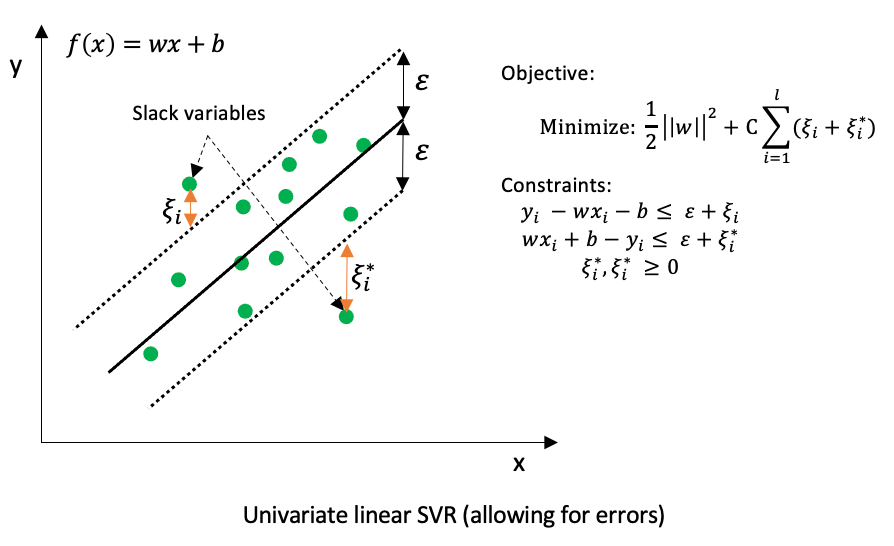
\includegraphics[scale=0.5]{images/SVR.png}
    \caption*{Esempio di SVR}
\end{figure} \newpage
\noindent In questo lavoro il modello è stato costruito usando gli iperparametri di default. Questi ultimi sono:
\begin{itemize}
    \item \textbf{kernel=rbf}: E' il tipo di Kernel\footnote{Funzione matematica usata per mappare i dati originali in uno spazio di dimensione superiore}{} utilizzato. Questo kernel valuta quanto due punti siano simili sulla base della loro distanza
    \item \textbf{degree=3}:  grado del polinomio utilizzato per la trasformazione dei dati nello spazio
    \item \textbf{gamma=scale}: coefficiente del kernel
    \item \textbf{coef0=0.0}: termine indipendente nel kernel
    \item \textbf{tol=0.001}: tolleranza per il criterio di arresto
    \item \textbf{C=1.0}: parametro di regolarizzazione
    \item \textbf{epsilon=0.1}:  controlla la tolleranza del modello nei confronti degli errori nella predizione
    \item \textbf{shrinking=True}: se abilitare o meno la riduzione del set di supporto
    \item \textbf{cache\_size=200}: dimensione della cache in MB
    \item \textbf{max\_iter=-1}: numero massimo di iterazioni. -1 indica nessun limite
\end{itemize}


\subsubsection{Decision Tree Regressor}

I Decision Tree Regressors sono modelli di regressione basati su alberi decisionali. Questi algoritmi suddividono ripetutamente il set di dati in base alle caratteristiche (features) per creare una struttura ad albero che rappresenta la relazione di decisione. Ogni nodo interno dell'albero rappresenta una decisione basata su una caratteristica, e le foglie dell'albero contengono i valori di output previsti.
\begin{figure}[H]
    \centering
    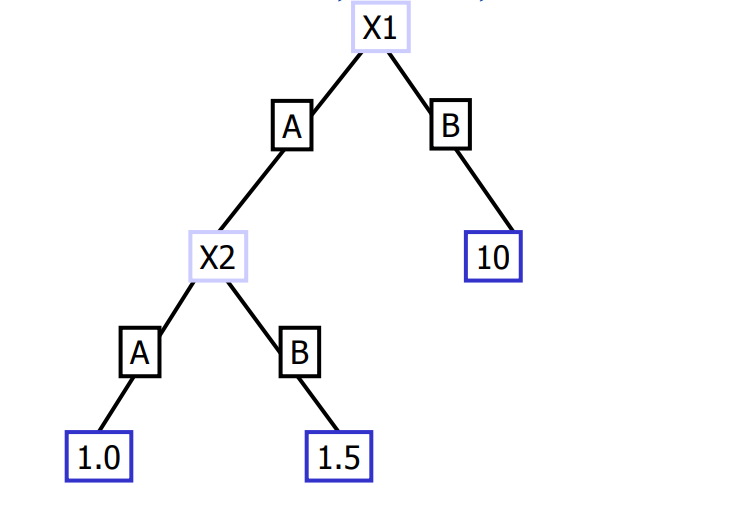
\includegraphics[scale=0.5]{images/DecisionTreeRegressor.png}
    \caption*{Esempio di albero decisionale di regressione}
\end{figure}

\noindent In questo lavoro due iperparametri sono stati decisi all'atto della costruzione del modello:
\begin{itemize}
    \item \textbf{max\_depth=5}: profondità massima dell'albero
    \item \textbf{random\_state=3}:  controlla la casualità nell'addestramento del modello. Quando viene fissato a un numero intero specifico l'addestramento del modello sarà deterministico, cioè produrrà gli stessi risultati in ogni esecuzione
\end{itemize}
\noindent mentre gli altri iperparametri sono stati lasciati ai valori di default:
\begin{itemize}
    \item \textbf{criterion=squared\_error}: Criterio per stabilire la qualità di una suddivisione
    \item \textbf{splitter=best}: Strategia per scegliere la suddivisione in ogni nodo
    \item \textbf{min\_samples\_split=2}: Numero minimo di campioni richiesti per suddividere un nodo interno
    \item \textbf{min\_samples\_leaf=1}: Numero minimo di campioni richiesti per essere in una foglia
    \item \textbf{min\_weight\_fraction\_leaf=0.0}: La frazione minima dei campioni totali (pesati) necessaria affinché si verifichi un nodo foglia
    \item \textbf{max\_features=None}: Numero di features da considerare quando si cerca la migliore suddivisione. None indica tutte
    \item \textbf{max\_leaf\_nodes=None}: Numero massimo di foglie. None indica nessun limite
    \item \textbf{min\_impurity\_decrease=0.0}: Un nodo verrà suddiviso se questa suddivisione induce una diminuzione dell'impurità maggiore o uguale a questo valore
    \item \textbf{ccp\_alpha=0.0}: Parametro di complessità usato per la potatura
    \item \textbf{monotonic\_constraints=None}: Vincoli monotoni sui valori delle features
\end{itemize}

\subsubsection{Random Forest Regressor}
I Random Forest Regressors sono modelli di regressione basati su alberi decisionali. Vengono costruiti su più alberi decisionali che combinano le loro previsioni per ottenere una previsione più accurata e stabile.
\begin{figure}[H]
    \centering
    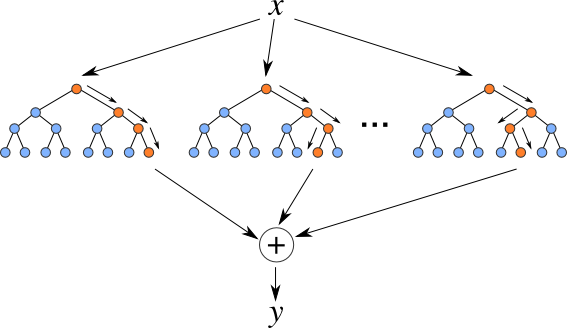
\includegraphics[scale=0.5]{images/RandomForestRegressor.png}
    \caption*{Esempio di Random Forest Regresor}
\end{figure}

\noindent In questo lavoro tre iperparametri sono stati decisi all'atto della costruzione del modello:
\begin{itemize}
    \item \textbf{n\_estimators=500}: numero di alberi nella foresta
    \item \textbf{max\_depth=5}: profondità massima dell'albero
    \item \textbf{random\_state=3}:  controlla la casualità nell'addestramento del modello. Quando viene fissato a un numero intero specifico l'addestramento del modello sarà deterministico, cioè produrrà gli stessi risultati in ogni esecuzione
\end{itemize}

\noindent mentre gli altri iperparametri sono stati lasciati ai valori di default:
\begin{itemize}
    \item \textbf{criterion=squared\_error}: Criterio per stabilire la qualità di una suddivisione
    \item \textbf{min\_samples\_split=2}: Numero minimo di campioni richiesti per suddividere un nodo interno
    \item \textbf{min\_samples\_leaf=1}: Numero minimo di campioni richiesti per essere in una foglia
    \item \textbf{min\_weight\_fraction\_leaf=0.0}: La frazione minima dei campioni totali (pesati) necessaria affinché si verifichi un nodo foglia
    \item \textbf{max\_features=1}: Numero di features da considerare quando si cerca la migliore suddivisione
    \item \textbf{max\_leaf\_nodes=None}: Numero massimo di foglie. None indica nessun limite
    \item \textbf{min\_impurity\_decrease=0.0}: Un nodo verrà suddiviso se questa suddivisione induce una diminuzione dell'impurità maggiore o uguale a questo valore
    \item \textbf{ccp\_alpha=0.0}: Parametro di complessità usato per la potatura
    \item \textbf{bootstrap=True}: Se utilizzare il bootstrap per la costruzione degli alberi
    \item \textbf{oob\_score=False}: Se calcolare l'errore out-of-bag
    \item \textbf{n\_jobs=None}: Numero di lavori da eseguire in parallelo. None indica 1
    \item \textbf{warm\_start=False}: Se utilizzare la soluzione precedente come inizializzazione
    \item \textbf{max\_samples=None}: Numero massimo di campioni da utilizzare per la costruzione di ciascun albero. None indica tutti
    \item \textbf{monotonic\_constraints=None}: Vincoli monotoni sui valori delle features
\end{itemize}
\newpage
\subsubsection{AdaBoost Regressor}
L'AdaBoost Regressor è un modello basato sull'algoritmo di boosting AdaBoost\footnote{Crea un modello forte combinando modelli più deboli, ognuno allenato su diverse parti del dataset}{}. Questo algoritmo costruisce un modello di previsione combinando più modelli di previsione più deboli.
\begin{figure}[H]
    \centering
    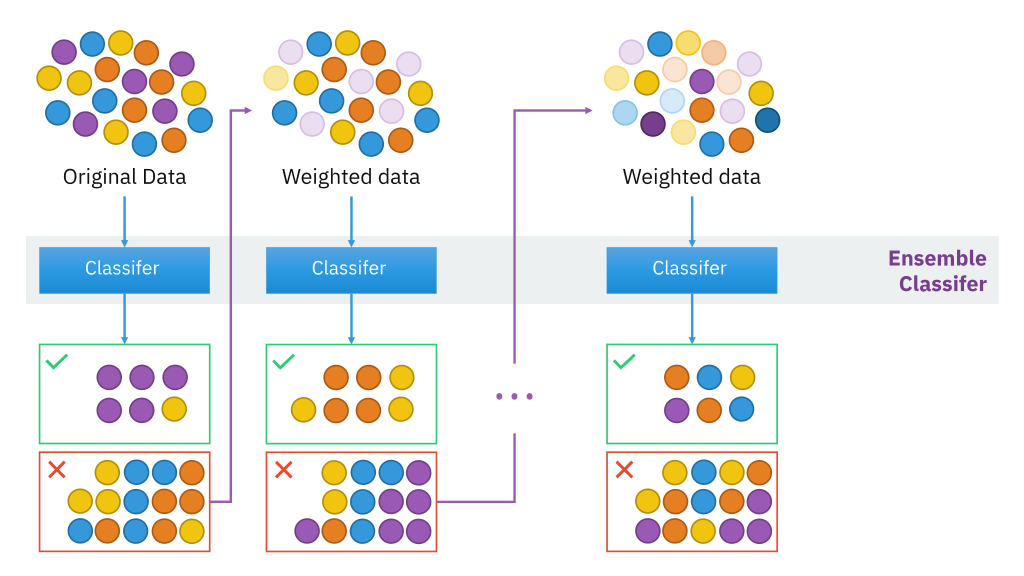
\includegraphics[scale=0.4]{images/AdaBoost.png}
    \caption*{Struttura di modello basato su AdaBoost}
\end{figure}

\noindent In questo lavoro due iperparametri sono stati decisi all'atto della costruzione del modello:

\begin{itemize}
    \item \textbf{n\_estimators=500}: numero di stimatori
    \item \textbf{random\_state=3}:  controlla la casualità nell'addestramento del modello. Quando viene fissato a un numero intero specifico l'addestramento del modello sarà deterministico, cioè produrrà gli stessi risultati in ogni esecuzione
\end{itemize}

\noindent mentre gli altri iperparametri sono stati lasciati ai valori di default:
\begin{itemize}
    \item \textbf{estimator=None}: stimatore base. Se None, viene utilizzato DecisionTreeRegressor
    \item \textbf{learning\_rate=1.0}: tasso di apprendimento
    \item \textbf{loss=linear}: funzione di perdita
\end{itemize}


    \newpage
    \section{Risultati}

In questo capitolo si analizzano i risultati degli esperimenti che sono stati condotti. I regressori utilizzati sono stati valutati utilizzando le seguenti metriche per la regressione:
\begin{itemize}
    %add the mathematic formula of each error
    \item \textbf{Mean Absolute Error (MAE)}: è la media della differenza assoluta tra le previsioni e i valori reali.
    \begin{equation*}
        MAE = \frac{1}{n} \sum_{i=1}^{n} |y_i - \hat{y}_i|
    \end{equation*}
    \item \textbf{Root Mean Squared Error (RMSE)}: è la radice quadrata della media della differenza tra le previsioni e i valori reali al quadrato.
    \begin{equation*}
        RMSE = \sqrt{\frac{1}{n} \sum_{i=1}^{n} (y_i - \hat{y}_i)^2}
    \end{equation*}
    \item \textbf{Mean Logarithmic Squared Error (MSLE)}: è la media del logaritmo dei quadrati degli errori.
    \begin{equation*}
        MSLE = \frac{1}{n} \sum_{i=1}^{n} (\log(y_i + 1) - \log(\hat{y}_i + 1))^2
    \end{equation*}
\end{itemize}

\subsection{Risultati ottenuti}

\begin{table}[H]
    \centering
    \begin{tabular}{|>{\centering\arraybackslash}m{5cm}|c|c|c|c|}
        \hline
        \textbf{Regressor} & \textbf{MAE} & \textbf{RMSE} & \textbf{MSLE} \\ [10pt]
        \hline
        SVR & 0.0288215 & 0.0008862 & 0.0008537 \\ [10pt]
        \hline
        Decision Tree & 0.0048531 & 0.0000969 & 0.0000918 \\ [10pt]
        \hline
        Random Forest & 0.0054369 & 0.0001088 & 0.0001026 \\ [10pt]
        \hline
        AdaBoost & 0.0071778 & 0.0001113 & 0.0001059 \\ [10pt]
        \hline
    \end{tabular}
    \caption{Risultati ottenuti}
    \label{tab:results}
\end{table}

\begin{table}[H]
    \centering
    \begin{tabular}{c c}
        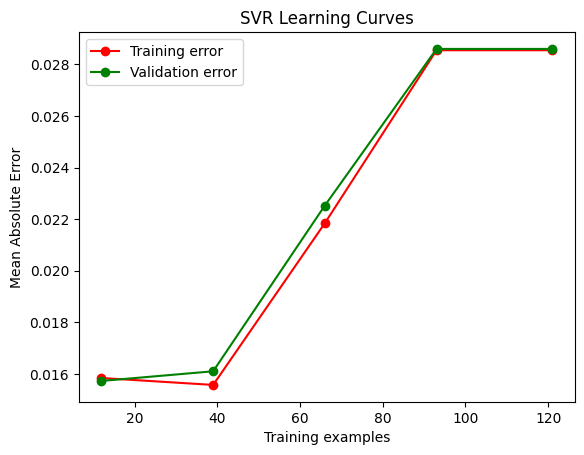
\includegraphics[scale=0.3]{images/SVR_lc.png} & 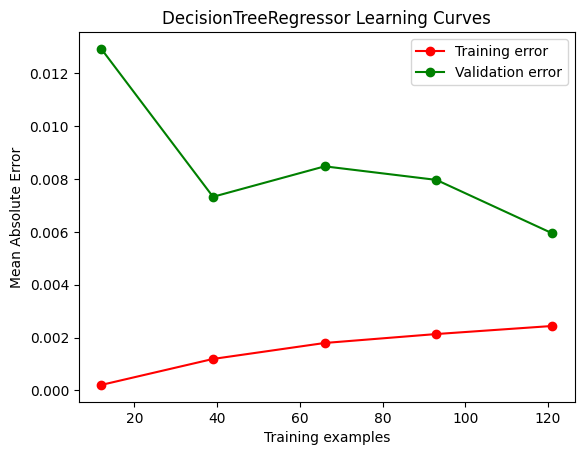
\includegraphics[scale=0.3]{images/DecisionTree_lc.png} \\
        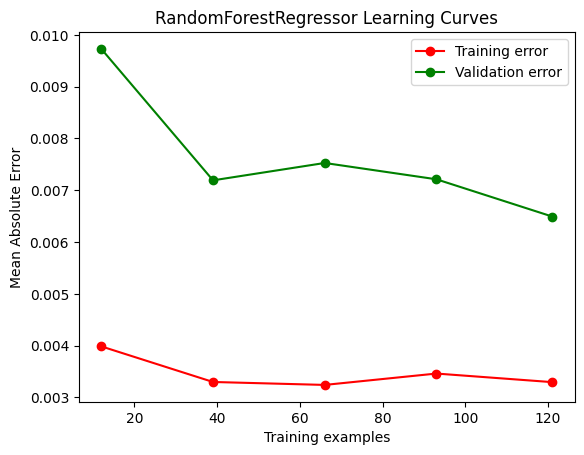
\includegraphics[scale=0.3]{images/RandomForestRegressor_lc.png} & 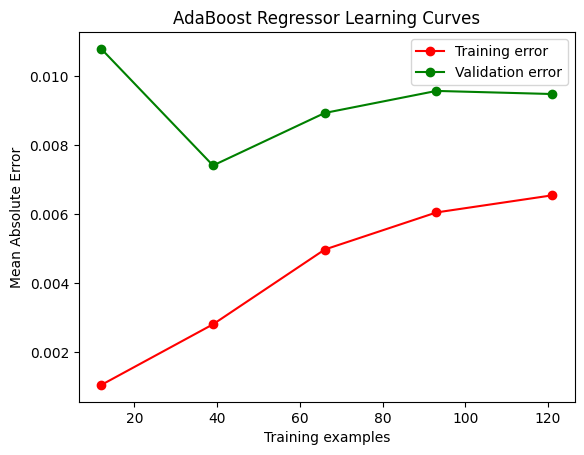
\includegraphics[scale=0.3]{images/AdaBoostRegressor_lc.png} \\
    \end{tabular}
    \caption{Learning curve dei regressori}
    \label{tab:lc}
\end{table}

\subsection{Analisi dei risultati}


    \paragraph{\textbf{SVR}.}
    Dal punto di vista delle metriche il regressore SVR ha ottenuto i peggiori risultati in termini di MAE, RMSE e MSLE. La learning curve mostra che il modello è in overfitting, infatti gli errori aumentano all'aumentare del numero di istanze.
   
   
    \paragraph{\textbf{Decision Tree Regressor}.}
    Dal punto di vista delle metriche, il Decision Tree Regressor ha ottenuto i migliori risultati. 
    La learning curve mostra una curva di training che aumenta all'aumentare del numero di istanze, mentre la curva di validation diminuisce. Le due curve si avvicinano, ma non si sovrappongono. Sembra esserci un leggero underfitting.
    \paragraph{\textbf{Random Forest Regressor}.}
    Dal punto di vista delle metriche il Random Forest Regressor risulta essere il secondo miglior modello.
    La learning curves di train e di validation set diminuiscono entrambe all'aumentare del numero di istanze, ma non si sovrappongono. Anche qui sembra esserci underfitting.
    \paragraph{\textbf{AdaBoost Regressor}.}
    Dal punto di vista delle metriche il AdaBoost Regressor ha ottenuto risultati peggiori rispetto al Random Forest Regressor ma migliori rispetto al SVR.
    La learning curve mostrano che il modello non è riuscito a generalizzare bene


\subsection{Conclusioni}
Il dataset sembra essere troppo piccolo per poter generalizzare bene i modelli. Inoltre, il dataset è molto sbilanciato, con pochi valori per ogni feature. Questo potrebbe essere un motivo per cui i modelli non generalizzano bene. Inoltre, i modelli non sono stati ottimizzati, quindi potrebbero essere migliorati mediante ricerca di iperparametri.
Per i risultati attuali, il Decision Tree Regressor è il modello migliore.
    \newpage
    
    
\noindent LFM1b\_artist è un dataset contenente informazioni riguardanti le interazioni tra utenti e artisti musicali.

\section*{DETASET ORIGINALE}

\subsection*{STATISTICHE DATASET}


Descrizione del dataset
\begin{table}[H]
    \centering
    \footnotesize
    \begin{tabularx}{\textwidth}{|c|X|}
        \hline
        \textbf{Feature} & \textbf{Descrizione} \\
        \hline
        n\_users & 120322 \\
        \hline
        n\_items & 3123496 \\
        \hline
        n\_inter & 65133026 \\
        \hline
        sparsity & 0.9998266933373666 \\
        \hline
    \end{tabularx}
    \caption{Informazioni sul dataset LFM1b\_artist}
    \label{tab:dataset_info}
\end{table}


\noindent Descrizione del knowledge graph
\begin{table}[H]
    \centering
    \footnotesize
    \begin{tabularx}{\textwidth}{|c|X|}
        \hline
        n\_ent\_head & 823213 \\
        \hline
        n\_ent\_tail & 353607 \\
        \hline
        n\_rel & 8 \\
        \hline
        n\_triple & 2114049 \\
        \hline
    \end{tabularx}
    \caption{Informazioni sul knowledge graph del dataset LFM1b\_artist}
    \label{tab:dataset_info}
\end{table}

\newpage
\noindent I nomi delle relazioni presenti nel knowledge graph sono i seguenti:
\begin{itemize}
    \item music.recording.artist
    \item music.recording.releases
    \item music.recording.producer
    \item music.recording.engineer
    \item music.recording.featured\_artists
    \item music.featured\_artist.recordings
    \item music.release.artist
    \item music.artist.release
\end{itemize}

\section*{DATASET PROCESSATO}

\subsection*{DESCRIZIONE}

\noindent Il dataset originale risultava essere troppo grande per le risorse a nostra disposizione, dunque è stato opportunamente processato. In paritcolare sono state svolte le seguenti operazioni
\begin{itemize}
    \item \textbf{Filtraggio:} il dataset è stato filtrato eliminando tutte le interazioni in cui erano coinvolti utenti e/o item con meno di 5 interazioni
    \item \textbf{Sampling:} dopo la fase di filtraggio, è stato effettuato un sampling casuale il cui scopo era quello di ridurre il numero di interazioni. In particolare sono stati selezionati casualmente 20000 utenti e 50000 item e sono state mantenute solo le interazioni in cui erano coinvolti utenti e gli item selezionati
\end{itemize}

\subsection*{STATISTICHE DATASET}


Descrizione del dataset
\begin{table}[H]
    \centering
    \footnotesize
    \begin{tabularx}{\textwidth}{|c|X|}
        \hline
        \textbf{Feature} & \textbf{Descrizione} \\
        \hline
        n\_users & 19481 \\
        \hline
        n\_items & 42547 \\
        \hline
        n\_inter & 900212 \\
        \hline
        sparsity & 0.0.9989313587429705 \\
        \hline
    \end{tabularx}
    \caption{Informazioni sul dataset LFM1b\_artist processato}
    \label{tab:dataset_info}
\end{table}


\noindent Descrizione del knowledge graph
\begin{table}[H]
    \centering
    \footnotesize
    \begin{tabularx}{\textwidth}{|c|X|}
        \hline
        n\_ent\_head & 15509 \\
        \hline
        n\_ent\_tail & 35156 \\
        \hline
        n\_rel & 5 \\
        \hline
        n\_triple & 46827 \\
        \hline
    \end{tabularx}
    \caption{Informazioni sul knowledge graph del dataset LFM1b\_artist processato}
    \label{tab:dataset_info}
\end{table}

\noindent I nomi delle relazioni presenti nel knowledge graph sono i seguenti:
\begin{itemize}
    \item music.recording.artist
    \item music.recording.releases
    \item music.recording.producer
    \item music.recording.engineer
    \item music.recording.featured\_artists
\end{itemize}


\newpage

\section*{ESECUZIONE DEI MODELLI E RISULTATI}

I modelli di recommendation sono stati eseguiti utilizzando questi parametri:
\begin{itemize}
    \item \textbf{Numero di epoche:} 1
    \item \textbf{Train batch size:} 4096
    \item \textbf{Eval batch size:} 1024
    \item \textbf{Numero neighbors per l'ItemKNN:} 20
\end{itemize}


Qui di seguito sono riportati i risultati ottenuti dai modelli di recommendation.
\begin{table}[H]
    \centering
    \footnotesize
    \begin{tabularx}{\textwidth}{|c|c|X|}
        \hline
        \textbf{Nome modello} & \textbf{Esito} & \textbf{Motivo fallimento} \\
        \hline
        ItemKNN & Successo &  \\
        \hline
        Pop & Successo &  \\
        \hline
        Random & Fallito &  Expected all tensors to be on the same device, but found at least two devices, cuda:0 and cpu! (when checking argument for argument tensors in method wrapper\_CUDA\_cat) \\
        \hline
        Simplex & Successo &  \\
        \hline
        ADMMSLIM & Fallito & Terminato in modo anomalo \\
        \hline
        BPR & Successo &  \\
        \hline
        DMF & Successo &  \\
        \hline
        ENMF & Successo &  \\
        \hline
        FISM & Successo &  \\
        \hline
        NCEPLRec & Successo &  \\
        \hline
        SLIMElasticNet & Fallito &  Expected all tensors to be on the same device, but found at least two devices, cuda:0 and cpu! (when checking argument for argument tensors in method wrapper\_CUDA\_cat) \\
        \hline
        CDAE & Successo &  \\
        \hline
        COnvNCF & Successo &  \\
        \hline
        DiffRec & Successo &  \\
        \hline
        EASE & Fallito & Terminato in modo anomalo \\
        \hline
        GCMC & Successo &  \\
        \hline
        LDiffRec & Successo &  \\
        \hline
        MacridVAE & Fallito &  CUDA out of memory. Tried to allocate 664.00 MiB \\
        \hline
        MultiDAE & Successo &  \\
        \hline
        MultiVAE & Successo &  \\
        \hline
        NAIS & Fallito & CUDA out of memory. Tried to allocate 3.97 GiB \\
        \hline
        NeuMF & Successo &  \\
        \hline
        NGCF & Successo &  \\
        \hline
        NNCF & Successo &  \\
        \hline
        LightGCN & Successo &  \\
        \hline
        RecVAE & Rimandato & Tempo di esecuzione non accettabile \\
        \hline
        DGCF & Successo &  \\
        \hline
        LINE & Successo &  \\
        \hline
        NCL & Fallito & No module faiss \\
        \hline
        SGL & Successo & \\
        \hline
        SpectralCF & Successo &  \\
        \hline
        CKE & Successo &  \\
        \hline
        CFKG & Successo &  \\
        \hline
        KGIN & Fallito & mismatch di versione tra PyTorch e torch\-scatter \\
        \hline
        KGNNLS & Successo &  \\
        \hline
        KTUP & Successo &  \\
        \hline
        MKR & Successo &  \\
        \hline
        RippleNet & Successo &  \\
        \hline
    \end{tabularx}
    \caption{Esiti di esecuzione dei modelli}
    \label{tab:dataset_info}
\end{table}



    \newpage
    \subsection{Configurazione}

\subsubsection{Parametri di running}
Qui di seguito vengono riportati i parametri di running dei vari esperimenti effettuati.


\noindent \textbf{Parametri di environment}


\noindent I parametri di environment servono per configurare l'ambiente di esecuzione.
\begin{itemize}
    \item \textbf{gpu\_id}: 0
    \item \textbf{worker}: 0
    \item \textbf{use\_gpu}: True
    \item \textbf{seed}: 2020
    \item \textbf{state}: INFO
    \item \textbf{encoding}: utf-8
    \item \textbf{reproducibility}: True
    \item \textbf{shuffle}: True
\end{itemize}


\noindent \textbf{Parametri di training}


\noindent I parametri di training servono per l'addestramento dei modelli.
\begin{itemize}
    \item \textbf{epochs}: 200
    \item \textbf{train\_batch\_size}: 2048
    \item \textbf{learner}: adam
    \item \textbf{learning\_rate}: .001
    \item \textbf{train\_neg\_sample\_args}: 
    \begin{itemize}
        \item \textbf{distribution}: uniform
        \item \textbf{sample\_num}: 1
        \item \textbf{dynamic}: False
        \item \textbf{candidate\_num}: 0
    \end{itemize}
    \item \textbf{eval\_step}: 1
    \item \textbf{stopping\_step}: 10
    \item \textbf{clip\_grad\_norm}: None
    \item \textbf{loss\_decimal\_place}: 4
    \item \textbf{weight\_decay}: .0
    \item \textbf{require\_pow}: False
    \item \textbf{enable\_amp}: False
    \item \textbf{enable\_scaler}: False
\end{itemize}


\noindent \textbf{Parametri di evaluation}


\noindent I parametri di evaluation servono per valutare i modelli.
\begin{itemize}
    \item \textbf{eval\_args}:
    \item \begin{itemize}
                \item \textbf{group\_by}: user
                \item \textbf{order}: RO
                \item \textbf{split}: RS : [0.8, 0.1, 0.1]
                \item \textbf{mode}: full
            \end{itemize}
    \item \textbf{repeatable}: False
    \item \textbf{metrics}: ['Recall', 'MRR', 'NDCG', 'Hit', 'MAP', 'Precision', 'GAUC', 'ItemCoverage', 'AveragePopularity', 'GiniIndex', 'ShannonEntropy', 'TailPercentage']
    \item \textbf{topk}: 10
    \item \textbf{valid\_metric}: MRR@10
    \item \textbf{eval\_batch\_size}: 4096
    \item \textbf{metric\_decimal\_place}: 4
\end{itemize}


\noindent \textbf{Iper parametri dei modelli}


\noindent Gli iper parametri dei modelli sono un insieme di parametri che vengono utilizzati per configurare i modelli. La loro configurazione può influenzare il risultato finale. Esistono delle tecniche di HyperTuning che permettono di trovare i migliori iper parametri per un determinato modello e dataset.
In questo caso si è scelto di utilizzare gli iper parametri di default



    \newpage
    \section{Emissioni}

Qui di seguito vengono riportate le emissioni di CO2 per ogni esperimento effettuato.

\begin{table}[H]
    \centering
    \footnotesize
    \setlength\tabcolsep{0pt}
    \begin{tabularx}{\textwidth}{|X|X|}
        \hline
        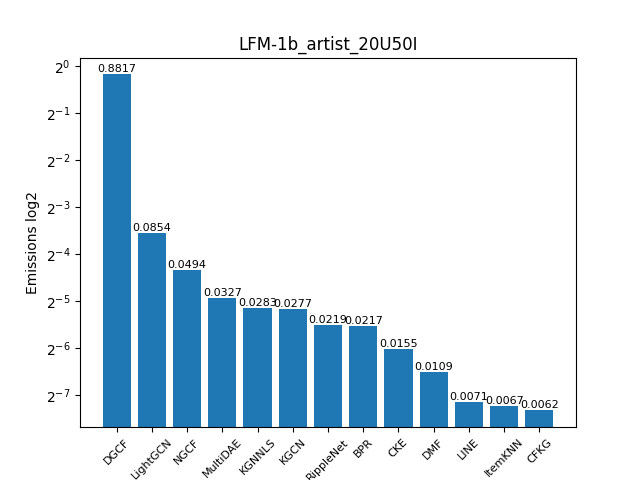
\includegraphics[width=\linewidth, trim=0 0 0 0]{images/emissions_LFM-1b_artist_20U50I.png} &
        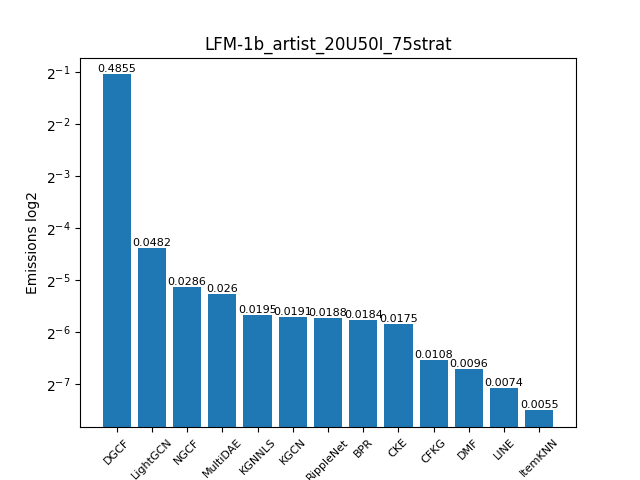
\includegraphics[width=\linewidth, trim=0 0 0 0]{images/emissions_LFM-1b_artist_20U50I_75strat.png} \\
        \hline
        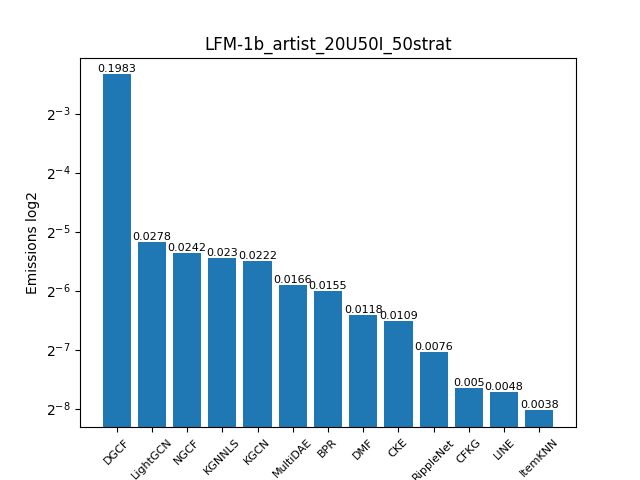
\includegraphics[width=\linewidth, trim=0 0 0 0]{images/emissions_LFM-1b_artist_20U50I_50strat.png} &
        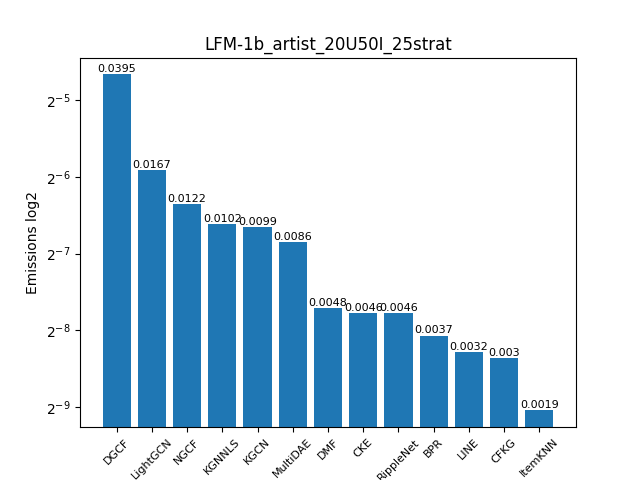
\includegraphics[width=\linewidth, trim=0 0 0 0]{images/emissions_LFM-1b_artist_20U50I_25strat.png} \\
        \hline
    \end{tabularx}
    \caption{Emissioni di CO2 per i vari dataset}
    \label{tab:emissions_info}
\end{table}

\noindent Si può subito notare come DGCF è il modello che emette più CO2 in assoluto.
In particolare con il dataset al 100\% e al 75\% DGCF emette circa 10 volte di più rispetto a LightGCN (il secondo per emissioni)
mentre con il dataset al 50\% emette circa 7 volte di più e con il dataset al 25\% emette circa 2 volte di più (sempre rispetto a LightGCN).
LightGCN e NCFG sono rispettivamente il secondo e il terzo modello che emettono più CO2.
Questi due modelli sono invece di tipo general, ma nonostante ciò emettono di più rispetto ad altri di tipo knowledge-aware, come per esempio il KGCN.
In generale possiamo vedere che ItemKNN,LINE e CFKG sono i modelli che emettono meno.
Per LINE e ItemKNN questo era abbastanza prevedibile in quanto modelli di tipo General. Interessante invece notare come CFKG, di tipo knowledge-aware, emetta meno di altri modelli di tipo General






    \newpage
    \subsection{Trade-off}


\subsubsection{Introduzione}
In questa sezione verranno analizzati i trade-off tra le varie metriche di valutazione e le emissioni di CO2 analizzando un dataset per volta.

Di seguito un elenco delle metriche con una piccola descrizione:
\begin{itemize}
    \item \textbf{Recall}: è una metrica che misura la capacità di un modello di raccomandare gli item rilevanti per un utente
    \item \textbf{NDCG}: è una metrica che misura la qualità delle raccomandazioni.
    \item \textbf{Gini Index}: è una metrica che misura l'equità nella distribuzione delle raccomandazioni. Un valore più vicino a zero indica una distribuzione più equa
    \item \textbf{Average Popularity}: è una metrica che misura la popolarità media degli item raccomandati. Un valore alto indica che le raccomandazioni sono concentrate su item popolari.
\end{itemize}

\subsubsection{LFM-1b\_artist\_20U50I}


\begin{table}[H]
    \centering
    \footnotesize
    \setlength\tabcolsep{0pt}
    \begin{tabularx}{\textwidth}{|X|X|}
        \hline
        \includegraphics[width=\linewidth, trim=0 0 0 0]{images/recall@10\_LFM-1b\_artist_20U50I.png} &
        \includegraphics[width=\linewidth, trim=0 0 0 0]{images/ndcg@10\_LFM-1b\_artist_20U50I.png} \\
        \hline
        \includegraphics[width=\linewidth, trim=0 0 0 0]{images/giniindex@10\_LFM-1b\_artist_20U50I.png} &
        \includegraphics[width=\linewidth, trim=0 0 0 0]{images/averagepopularity@10\_LFM-1b\_artist_20U50I.png} \\
        \hline
    \end{tabularx}
    \caption{Trade-off con il dataset LFM-1b\_artist\_20U50I}
    \label{tab:emissions_info}
\end{table}

\noindent Come già visto precedentemente, DGCF è il modello che emette di più. Nonostante ciò possiamo notare che per la recall e l'ndcg le sue performance risultano peggiori rispetto ad algoritmi più semplici come l'ItemKNN che risulta essere uno degli algoritmi che emette meno e performa meglio in queste metriche.
Per quanto riguarda il Gini Index possiamo notare che DGCF si comporta meglio di molti altri modelli ma l'ItemKNN e LINE risultano essere migliori di quest'ultimo. LINE è il miglior algoritmo.
Infine, per quanto riguarda l'Average Popularity, anche in questo caso possiamo notare anche che DGCF performa meglio di altri modelli, ma LINE risulta il miglior in assoluto ed è uno degli algoritmi che emette meno.


\subsubsection{LFM-1b\_artist\_20U50I\_75strat}


\begin{table}[H]
    \centering
    \footnotesize
    \setlength\tabcolsep{0pt}
    \begin{tabularx}{\textwidth}{|X|X|}
        \hline
        \includegraphics[width=\linewidth, trim=0 0 0 0]{images/recall@10\_LFM-1b\_artist_20U50I\_75strat.png} &
        \includegraphics[width=\linewidth, trim=0 0 0 0]{images/ndcg@10\_LFM-1b\_artist_20U50I\_75strat.png} \\
        \hline
        \includegraphics[width=\linewidth, trim=0 0 0 0]{images/giniindex@10\_LFM-1b\_artist_20U50I\_75strat.png} &
        \includegraphics[width=\linewidth, trim=0 0 0 0]{images/averagepopularity@10\_LFM-1b\_artist_20U50I\_75strat.png} \\
        \hline
    \end{tabularx}
    \caption{Trade-off con il dataset LFM-1b\_artist\_20U50I\_75strat}
    \label{tab:emissions_info}
\end{table}


\noindent Come già visto precedentemente, DGCF è il modello che emette di più. Nonostante ciò possiamo notare che per la recall e l'ndcg le sue performance risultano peggiori rispetto ad algoritmi più semplici come l'ItemKNN che risulta essere uno degli algoritmi che emette meno e performa meglio in queste metriche.
Per quanto riguarda il Gini Index possiamo notare che DGCF si comporta meglio di molti altri modelli ma l'ItemKNN e LINE risultano essere migliori di quest'ultimo. ItemKNN è il miglior algoritmo.
Infine, per quanto riguarda l'Average Popularity, anche in questo caso possiamo notare anche che DGCF performa meglio di altri modelli, ma LINE risulta il miglior in assoluto ed è uno degli algoritmi che emette meno.





\subsubsection{LFM-1b\_artist\_20U50I\_50strat}


\begin{table}[H]
    \centering
    \footnotesize
    \setlength\tabcolsep{0pt}
    \begin{tabularx}{\textwidth}{|X|X|}
        \hline
        \includegraphics[width=\linewidth, trim=0 0 0 0]{images/recall@10\_LFM-1b\_artist_20U50I\_50strat.png} &
        \includegraphics[width=\linewidth, trim=0 0 0 0]{images/ndcg@10\_LFM-1b\_artist_20U50I\_50strat.png} \\
        \hline
        \includegraphics[width=\linewidth, trim=0 0 0 0]{images/giniindex@10\_LFM-1b\_artist_20U50I\_50strat.png} &
        \includegraphics[width=\linewidth, trim=0 0 0 0]{images/averagepopularity@10\_LFM-1b\_artist_20U50I\_50strat.png} \\
        \hline
    \end{tabularx}
    \caption{Trade-off con il dataset LFM-1b\_artist\_20U50I\_50strat}
    \label{tab:emissions_info}
\end{table}


\noindent Come già visto precedentemente, DGCF è il modello che emette di più. Nonostante ciò possiamo notare che per la recall e l'ndcg le sue performance risultano peggiori rispetto ad altri algoritmi che emettono meno come CKE e CKFG(anch'essi di tipo Knowledge-Aware)..
Per quanto riguarda il Gini Index possiamo notare che DGCF si comporta meglio di molti altri modelli ma l'ItemKNN risulta essere migliore di quest'ultimo ed il migliore in assoluto.
Infine, per quanto riguarda l'Average Popularity, anche in questo caso possiamo notare anche che DGCF performa meglio di altri modelli, ma LINE risulta il miglior in assoluto ed è uno degli algoritmi che emette meno.



\subsubsection{LFM-1b\_artist\_20U50I\_25strat}


\begin{table}[H]
    \centering
    \footnotesize
    \setlength\tabcolsep{0pt}
    \begin{tabularx}{\textwidth}{|X|X|}
        \hline
        \includegraphics[width=\linewidth, trim=0 0 0 0]{images/recall@10\_LFM-1b\_artist_20U50I\_25strat.png} &
        \includegraphics[width=\linewidth, trim=0 0 0 0]{images/ndcg@10\_LFM-1b\_artist_20U50I\_25strat.png} \\
        \hline
        \includegraphics[width=\linewidth, trim=0 0 0 0]{images/giniindex@10\_LFM-1b\_artist_20U50I\_25strat.png} &
        \includegraphics[width=\linewidth, trim=0 0 0 0]{images/averagepopularity@10\_LFM-1b\_artist_20U50I\_25strat.png} \\
        \hline
    \end{tabularx}
    \caption{Trade-off con il dataset LFM-1b\_artist\_20U50I\_25strat}
    \label{tab:emissions_info}
\end{table}


\noindent Come già visto precedentemente, DGCF è il modello che emette di più. Nonostante ciò possiamo notare che per la recall e l'ndcg le sue performance risultano peggiori rispetto ad altri algoritmi che emettono meno come CKE e CKFG (anch'essi di tipo Knowledge-Aware).
Per quanto riguarda il Gini Index possiamo notare che DGCF si comporta meglio di molti altri modelli ma l'ItemKNN risulta essere di quest'ultimo migliore ed il migliore in assoluto.
Infine, per quanto riguarda l'Average Popularity, in questo caso possiamo notare anche che DGCF è uno dei peggiori mentre ItemKNN risulta il miglior in assoluto ed è l'algoritmo che emette meno.


\subsubsection{ml-10m\_50U10I}


\begin{table}[H]
    \centering
    \footnotesize
    \setlength\tabcolsep{0pt}
    \begin{tabularx}{\textwidth}{|X|X|}
        \hline
        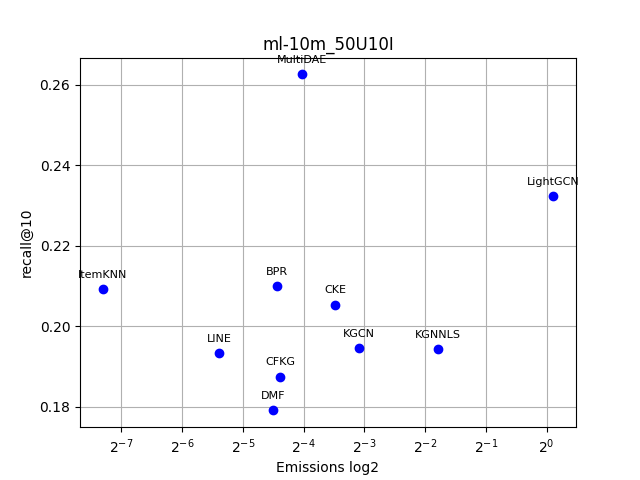
\includegraphics[width=\linewidth, trim=0 0 0 0]{images/recall@10_ml-10m_50U10I.png} &
        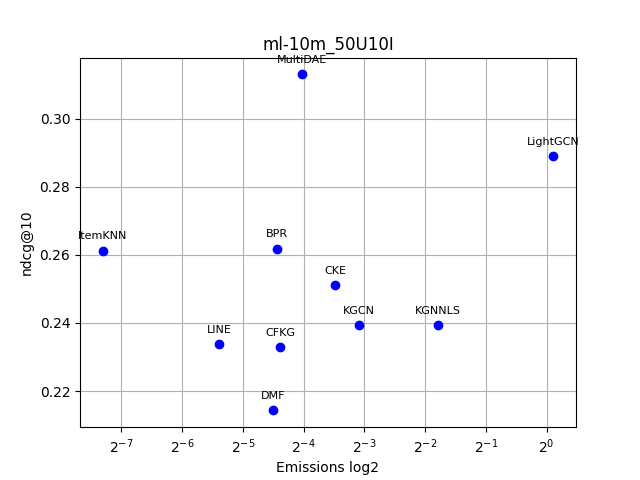
\includegraphics[width=\linewidth, trim=0 0 0 0]{images/ndcg@10_ml-10m_50U10I.png} \\
        \hline
        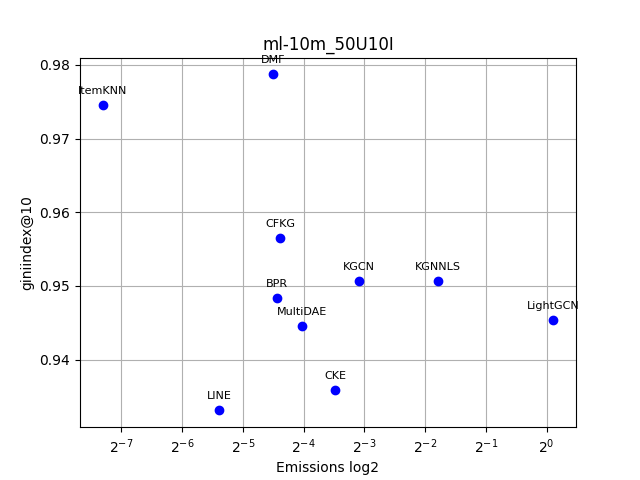
\includegraphics[width=\linewidth, trim=0 0 0 0]{images/giniindex@10_ml-10m_50U10I.png} &
        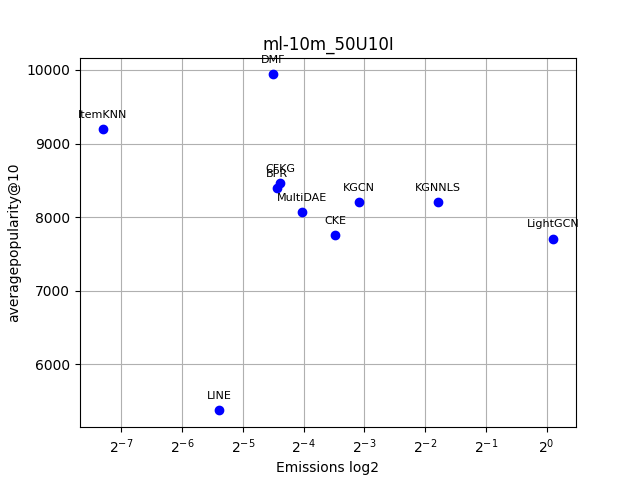
\includegraphics[width=\linewidth, trim=0 0 0 0]{images/averagepopularity@10_ml-10m_50U10I.png} \\
        \hline
    \end{tabularx}
    \caption{Trade-off con il dataset ml-10m\_50U10I}
    \label{tab:emissions_info}
\end{table}

\noindent LightGCN è l'algoritmo che emette di più, osservando i valori da 5 a circa 180 volte rispetto agli altri modelli.
Emissioni cosi alte non sono però giustificate. Nelle metriche di recall e ndcg LightGCN è il secondo migliore, ma la differenza rispetto al primo è molto bassa e quindi non giustifica emissioni così alte.
ItemKNN si conferma uno dei migliori algoritmi per queste due metriche in quanto emette meno ed è uno dei più performanti.
Per quanto riguarda le metriche di Gini Index e Average Popularity possiamo notare che LightGCN è uno di migliori, ma anche in questo caso la differenza rispetto ad altri modelli non giustifica emissioni così alte. ItemKNN si conferma con il secondo peggior modello come punteggi. Line risulta essere il migliore in quanto è il secondo per basse emissioni ed ottiene i punteggi migliori. 

\subsubsection{Conclusioni}

Si può facilmente notare come il trade-off emissioni-performance sia decisamente a svantaggio dell'DGCF. Infatti, a fronte di emissioni molto elevate, le performance risultato spesso essere peggiori di modelli molto più semplici.
Con i due dataset più grandi possiamo notare come in generale ItemKNN risulti essere uno degli algoritmi con il miglior trade-off emissioni-performance nelle metriche di ranking, mentre LINE risulta essere il migliore nelle metriche di popolarità e equità nelle distribuzioni.
Al diminuire della dimensione del dataset DGCF comincia a comportarsi meglio nelle metriche di popolarità e equità, ma le sue emissioni rimangono sempre molto alte e non giustificano una possibile scelta di questo modello.
ItemKNN comincia a non performare bene nelle metriche di ranking, mentre migliora nelle metriche di popolarità e equità, arrivando anche a risultare il migliore


    \newpage
    \subsection{Regressore}

\subsubsection{Dataset originale}


\noindent \textbf{Dataset completo}


\noindent Il nuovo dataset presenta i seguenti valori:
\begin{itemize}
    \item \textbf{n\_users}: [19841, 22155, 23679, 50000, 6040]
    \item \textbf{n\_items}: [42457, 24878, 33653, 38932, 54458, 4414, 10000 3706]
    \item \textbf{n\_inter}: [900212, 218457, 440620, 667850, 1465871, 1048575, 7053774, 1000209]
    \item \textbf{sparsity}: [0.99893136, 0.99955742, 0.9993401, 0.99913541, 0.99878504, 0.98996762,
    0.98589245, 0.95531637]
    \item \textbf{kg\_entities}: [50665, 32907, 42031, 47308, 26315, 0, 175646, 79347]
    \item \textbf{kg\_relations}: [5, 16, 0, 31, 49]
    \item \textbf{kg\_triples}: [46827, 29822, 38491, 43559, 96476, 0, 521125, 385923]
    \item \textbf{kg\_items}: [816701, 11446, 0, 10601, 3655]
    \item \textbf{cpu\_cores}: [12, 4]
    \item \textbf{ram\_size}: [64, 16, 27.40581512]
    \item \textbf{is\_gpu}: [1, 0]
\end{itemize}

\noindent Si può dunque notare un miglioramento per quanto riguarda la varietà dei valori rispetto al passato

\noindent I nuovi dati hanno portato alla seguente distribuzione dei dati (qui di seguito visualizzata):
\begin{figure}[H]
    \centering
    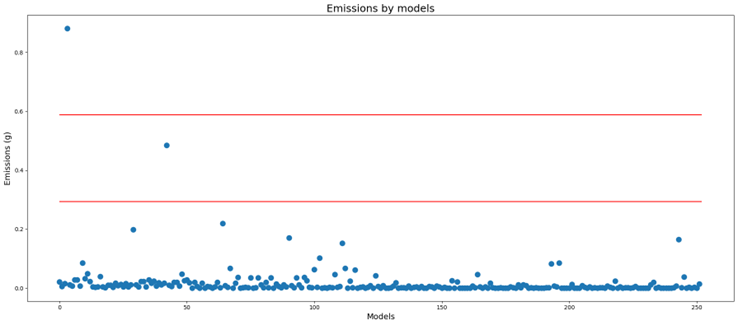
\includegraphics[scale=0.25]{images/nuova-situazione.png}
    \caption{Distribuzione delle emissioni nel dataset completo}
\end{figure}

\noindent Come è possibile notare però, i nuovi esperimenti hanno portato a un'ulteriore sbilanciamento nel dataset, in quanto tutti gli esperimenti con DGCF e altri modelli svettano sui risultati degli altri modelli in emissioni.
Questo si riflette nei risultati ottenuti dai modelli di regressione. Per quanto riguarda i modelli,
sono stati eseguti addestramenti con diversi split tra training e test set.


\noindent\textbf{Split 50/50}

\begin{table}[H]
    \centering
    \begin{tabular}{|>{\centering\arraybackslash}m{5cm}|c|c|c|c|}
        \hline
        \textbf{Regressor} & \textbf{MAE} & \textbf{RMSE} & \textbf{MSLE} \\ [10pt]
        \hline
        SVR & 0.1053920 & 0.0207610 & 0.0131238 \\ [10pt]
        \hline
        Decision Tree & 0.0369020 & 0.0149577 & 0.0079782 \\ [10pt]
        \hline
        Random Forest & 0.0338687 & 0.0151556 & 0.0077735 \\ [10pt]
        \hline
        AdaBoost & 0.0397532 & 0.0148615 & 0.0079069 \\ [10pt]
        \hline
    \end{tabular}
    \caption{Risultati ottenuti con il nuovo dataset split 50/50}
    \label{tab:results}
\end{table}

\begin{table}[H]
    \centering
    \footnotesize
    \setlength\tabcolsep{0pt}
    \begin{tabularx}{\textwidth}{|X|X|}
        \hline
        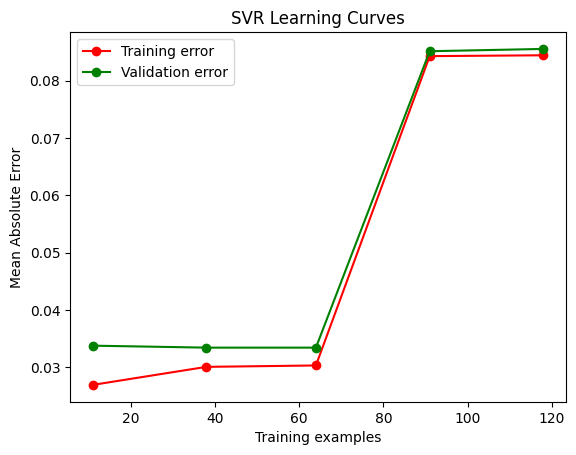
\includegraphics[width=\linewidth, trim=0 0 0 0]{images/SVR_lc50.png} &
        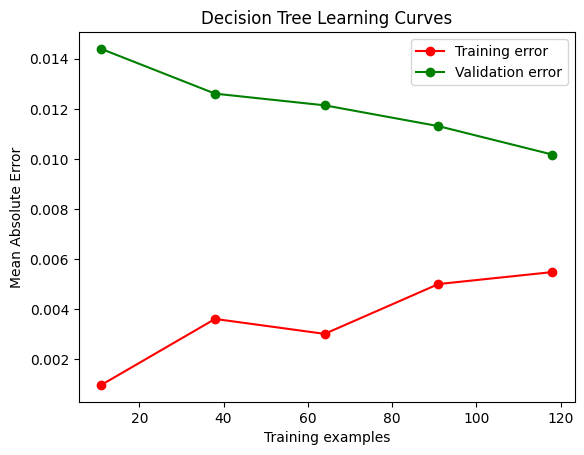
\includegraphics[width=\linewidth, trim=0 0 0 0]{images/DecisionTree_lc50.png} \\
        \hline
        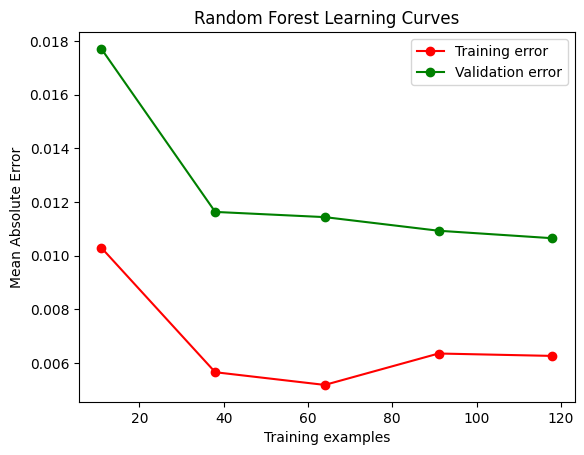
\includegraphics[width=\linewidth, trim=0 0 0 0]{images/RandomForest_lc50.png} &
        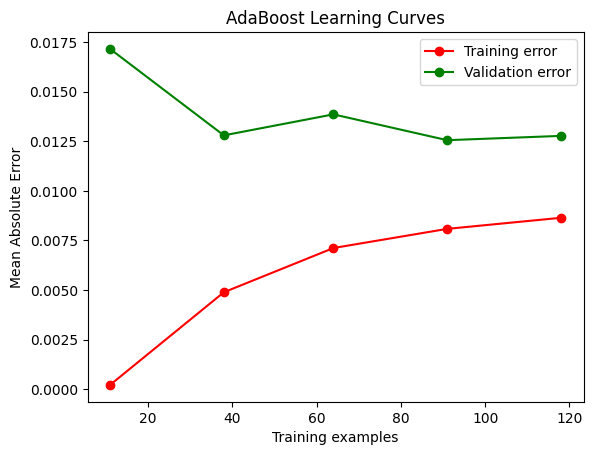
\includegraphics[width=\linewidth, trim=0 0 0 0]{images/AdaBoost_lc50.png} \\
        \hline
    \end{tabularx}
    \caption{Learning Curves con il nuovo dataset split 50/50}
    \label{tab:emissions_info}
\end{table}

\paragraph{\textbf{SVR}.}
Dal punto di vista delle metriche il regressore SVR ha ottenuto i peggiori risultati in termini di MAE, RMSE e MSLE. La learning curve mostra che il modello non è in grado di generalizzare, entrambe le curve crescono all'aumentare delle istanze.

\paragraph{\textbf{Decision Tree Regressor}.}
Dal punto di vista delle metriche, il Decision Tree Regressor ha ottenuto i risultati secondi al Random Forest Regressor. 
La learning curve mostra che la curva di training aumenta all'aumentare del numero di istanze mentre quella di validation diminuisce. Il modello dunque non ha generalizzato bene.
\paragraph{\textbf{Random Forest Regressor}.}
Dal punto di vista delle metriche il Random Forest Regressor risulta essere il miglior modello.
La learning curves di train e di validation set diminuiscono all'aumentare del numero di istanze. Quella di training tra 60 in poi aumenta ma intorno a 100 di stabilizza. Il modello sembra cominciare a generalizzare.
\paragraph{\textbf{AdaBoost Regressor}.}
Dal punto di vista delle metriche il AdaBoost Regressor ha ottenuto risultati peggiori rispetto al Decision Tree Regressor ma migliori rispetto al SVR.
La learning curve mostrano che il modello non è riuscito a generalizzare bene
in quanto la curva di validation aumenta e diminuisce all'aumentare delle istanze, mentre quella di training aumenta.

\paragraph{\textbf{Conclusioni}} Random Forest sembra essere il migliore sia dal punto di vista delle metriche che delle curve. Segue dietro il Decision Tree. AdaBoost e SVR non sono riusciti a generalizzare bene.
\newpage


\noindent\textbf{Split 60/40}

\begin{table}[H]
    \centering
    \begin{tabular}{|>{\centering\arraybackslash}m{5cm}|c|c|c|c|}
        \hline
        \textbf{Regressor} & \textbf{MAE} & \textbf{RMSE} & \textbf{MSLE} \\ [10pt]
        \hline
        SVR & 0.1082652 & 0.0237656 & 0.0144029 \\ [10pt]
        \hline
        Decision Tree & 0.0439202 & 0.0183129 & 0.0096602 \\ [10pt]
        \hline
        Random Forest & 0.0405412 & 0.0188566 & 0.0096752 \\ [10pt]
        \hline
        AdaBoost & 0.0519845 & 0.0186018 & 0.0099135 \\ [10pt]
        \hline
    \end{tabular}
    \caption{Risultati ottenuti con il nuovo dataset split 60/40}
    \label{tab:results}
\end{table}

\begin{table}[H]
    \centering
    \footnotesize
    \setlength\tabcolsep{0pt}
    \begin{tabularx}{\textwidth}{|X|X|}
        \hline
        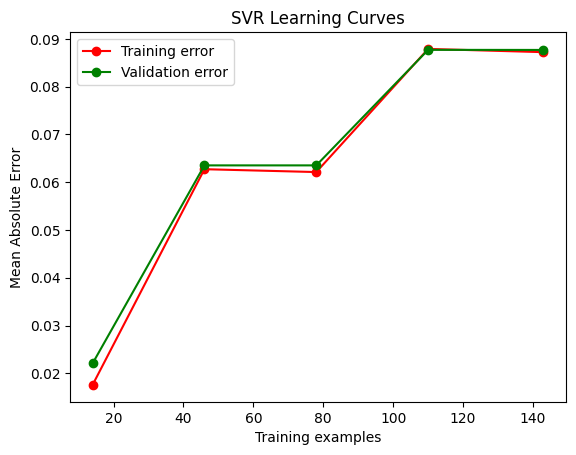
\includegraphics[width=\linewidth, trim=0 0 0 0]{images/SVR_lc60.png} &
        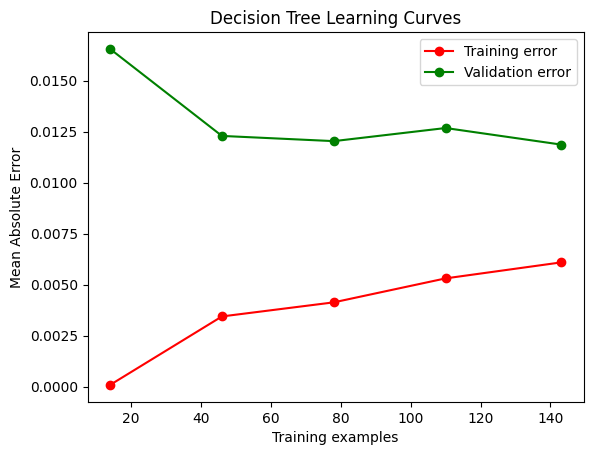
\includegraphics[width=\linewidth, trim=0 0 0 0]{images/DecisionTree_lc60.png} \\
        \hline
        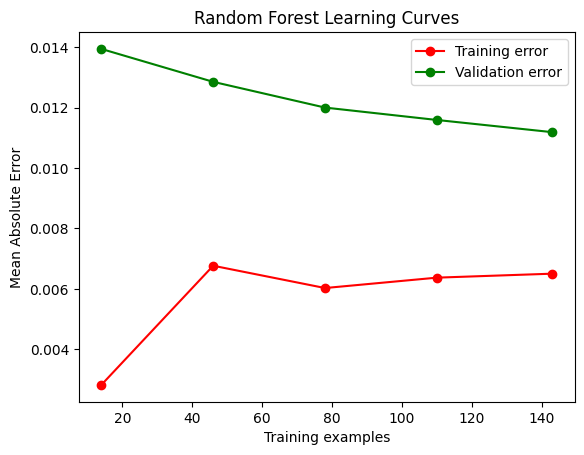
\includegraphics[width=\linewidth, trim=0 0 0 0]{images/RandomForest_lc60.png} &
        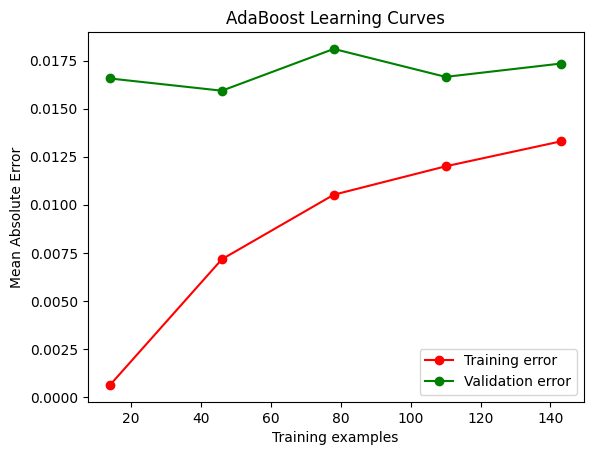
\includegraphics[width=\linewidth, trim=0 0 0 0]{images/AdaBoost_lc60.png} \\
        \hline
    \end{tabularx}
    \caption{Learning Curves con il nuovo dataset split 60/40}
    \label{tab:emissions_info}
\end{table}

\paragraph{\textbf{SVR}.}
Dal punto di vista delle metriche il regressore SVR ha ottenuto i peggiori risultati in termini di MAE, RMSE e MSLE. La learning curve mostra che il modello non è in grado di generalizzare, entrambe le curve crescono all'aumentare delle istanze.

\paragraph{\textbf{Decision Tree Regressor}.}
Dal punto di vista delle metriche, il Decision Tree Regressor ha ottenuto i risultati secondi al Random Forest Regressor. 
La learning curve mostra che la curva di training aumenta all'aumentare del numero di istanze mentre quella di validation diminuisce. Il modello dunque non ha generalizzato bene.
\paragraph{\textbf{Random Forest Regressor}.}
Dal punto di vista delle metriche il Random Forest Regressor risulta essere il miglior modello.
La learning curves di training diminuisce all'aumentare del numero di istanze. Quella di training intorno a 80 comincia ad aumentare leggermente e a stabilizzarsi.
\paragraph{\textbf{AdaBoost Regressor}.}
Dal punto di vista delle metriche il AdaBoost Regressor ha ottenuto risultati peggiori rispetto al Decision Tree Regressor ma migliori rispetto al SVR.
La learning curve mostrano che il modello non è riuscito a generalizzare bene
in quanto la curva di validation aumenta e diminuisce all'aumentare delle istanze, mentre quella di training aumenta.

\paragraph{\textbf{Conclusioni}} Random Forest sembra essere il migliore sia dal punto di vista delle metriche che delle curve. Segue dietro il Decision Tree. AdaBoost e SVR non sono riusciti a generalizzare bene. In generale i modelli peggiorano rispetto allo split 50/50.
\newpage



\noindent\textbf{Split 70/30}

\begin{table}[H]
    \centering
    \begin{tabular}{|>{\centering\arraybackslash}m{5cm}|c|c|c|c|}
        \hline
        \textbf{Regressor} & \textbf{MAE} & \textbf{RMSE} & \textbf{MSLE} \\ [10pt]
        \hline
        SVR & 0.1103392 & 0.0268736 & 0.0154947 \\ [10pt]
        \hline
        Decision Tree & 0.0419923 & 0.0139534 & 0.0067713 \\ [10pt]
        \hline
        Random Forest & 0.0410102 & 0.0179366 & 0.0081916 \\ [10pt]
        \hline
        AdaBoost & 0.0486434 & 0.0160941 & 0.0074143 \\ [10pt]
        \hline
    \end{tabular}
    \caption{Risultati ottenuti con il nuovo dataset split 70/30}
    \label{tab:results} 
\end{table}

\begin{table}[H]
    \centering
    \footnotesize
    \setlength\tabcolsep{0pt}
    \begin{tabularx}{\textwidth}{|X|X|}
        \hline
        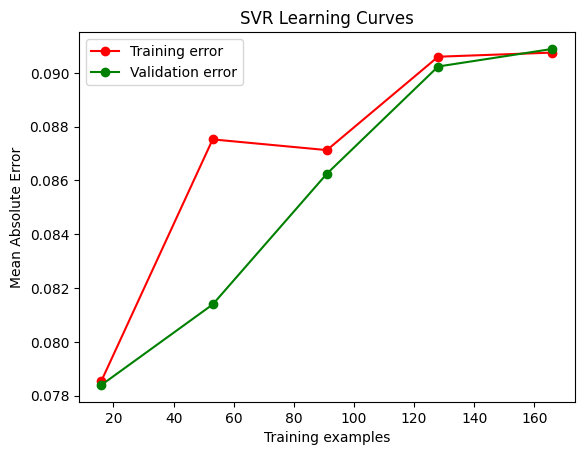
\includegraphics[width=\linewidth, trim=0 0 0 0]{images/SVR_lc70.png} &
        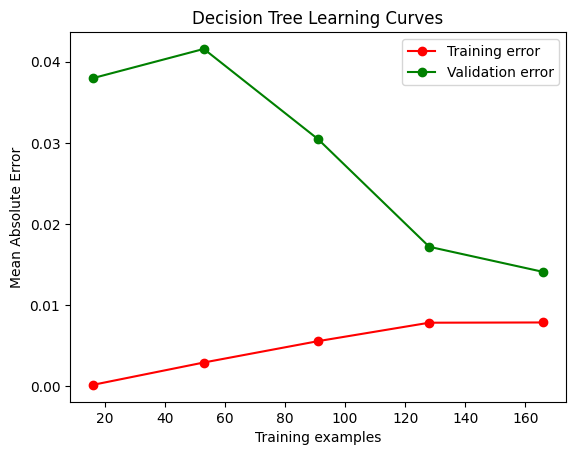
\includegraphics[width=\linewidth, trim=0 0 0 0]{images/DecisionTree_lc70.png} \\
        \hline
        \includegraphics[width=\linewidth, trim=0 0 0 0]{images/RandomForestRegressor_lc70.png} &
        \includegraphics[width=\linewidth, trim=0 0 0 0]{images/AdaBoostRegressor_lc70.png} \\
        \hline
    \end{tabularx}
    \caption{Learning Curves con il nuovo dataset split 70/30}
    \label{tab:emissions_info}
\end{table}

\paragraph{\textbf{SVR}.}
Dal punto di vista delle metriche il regressore SVR ha ottenuto i peggiori risultati in termini di MAE, RMSE e MSLE. La learning curve mostra che il modello non è in grado di generalizare, l'errore aumenta all'aumentare delle istanze.

\paragraph{\textbf{Decision Tree Regressor}.}
Dal punto di vista delle metriche di RMSE e MSLE, il Decision Tree Regressor ha ottenuto i migliori risultati. 
La learning curve mostra una curva di training che aumenta all'aumentare del numero di istanze, mentre la curva di validation diminuisce. Le due curve si avvicinano, ma non si sovrappongono. Sembra esserci un leggero miglioramento rispetto al passato.
\paragraph{\textbf{Random Forest Regressor}.}
Dal punto di vista delle metriche il Random Forest Regressor risulta essere il secondo miglior modello, tranne per MAE dove è il migliore.
La learning curves di train e di validation set diminuiscono entrambe all'aumentare del numero di istanze, ma non si sovrappongono. Anche qui rispetto al passato si nota un leggero miglioramento.
\paragraph{\textbf{AdaBoost Regressor}.}
Dal punto di vista delle metriche il AdaBoost Regressor ha ottenuto risultati peggiori rispetto al Random Forest Regressor e al Decision Tree Regressor ma migliori rispetto al SVR.
La learning curve mostrano che il modello non è riuscito a generalizzare bene ma si è comportato meglio rispetto al passato.


\paragraph{\textbf{Conclusioni}} Vi è un generale miglioramento rispetto allo split 60/40. Random Forest e Decision Tree sono i migliori modelli. AdaBoost e SVR non sono riusciti a generalizzare bene.



\noindent\textbf{Split 80/20}

\begin{table}[H]
    \centering
    \begin{tabular}{|>{\centering\arraybackslash}m{5cm}|c|c|c|c|}
        \hline
        \textbf{Regressor} & \textbf{MAE} & \textbf{RMSE} & \textbf{MSLE} \\ [10pt]
        \hline
        SVR & 0.1211949 & 0.0364312 & 0.0196837 \\ [10pt]
        \hline
        Decision Tree & 0.0511053 & 0.0211890 & 0.0095072 \\ [10pt]
        \hline
        Random Forest & 0.0538403 & 0.0262660 & 0.0118334 \\ [10pt]
        \hline
        AdaBoost & 0.0617220 & 0.0230938 & 0.0104140 \\ [10pt]
        \hline
    \end{tabular}
    \caption{Risultati ottenuti con il nuovo dataset split 80/20}
    \label{tab:results} 
\end{table}

\begin{table}[H]
    \centering
    \footnotesize
    \setlength\tabcolsep{0pt}
    \begin{tabularx}{\textwidth}{|X|X|}
        \hline
        \includegraphics[width=\linewidth, trim=0 0 0 0]{images/SVR_lc80.png} &
        \includegraphics[width=\linewidth, trim=0 0 0 0]{images/DecisionTree_lc80.png} \\
        \hline
        \includegraphics[width=\linewidth, trim=0 0 0 0]{images/RandomForest_lc80.png} &
        \includegraphics[width=\linewidth, trim=0 0 0 0]{images/AdaBoost_lc80.png} \\
        \hline
    \end{tabularx}
    \caption{Learning Curves con il nuovo dataset split 80/20}
    \label{tab:emissions_info}
\end{table}

\paragraph{\textbf{SVR}.}
Dal punto di vista delle metriche il regressore SVR ha ottenuto i peggiori risultati in termini di MAE, RMSE e MSLE. La learning curve di validation aumenta all'aumentare delle istanze, mentre quella di training è più instabile. Il modello non è riuscito a generalizzare bene.

\paragraph{\textbf{Decision Tree Regressor}.}
Dal punto di vista delle metriche il Decision Tree Regressor ha ottenuto i migliori risultati. 
La learning curve mostra una curva di training che aumenta all'aumentare del numero di istanze cominciando una lenta discesa verso le 150 istanze, mentre la curva di validation diminuisce. Le due curve si avvicinano, Sembra che il modello cominci a generalizzare.
\paragraph{\textbf{Random Forest Regressor}.}
Random Forest Regressor è secondo migliore in MAE, terzo in RMSE e MSLE.
La learning curves di train e di validation set diminuiscono entrambe all'aumentare del numero di istanze, ma non si sovrappongono. Comportamento analogo al passato.
\paragraph{\textbf{AdaBoost Regressor}.}
AdaBoost è il secondo migliore in RMSE e MSLE, terzo in MAE.
La learning curve mostrano che il modello non è riuscito a generalizzare bene.


\paragraph{\textbf{Conclusioni}} Decision Tree è il miglior modello. Tuttavia rispetto allo split precedente vi è un generale peggioramento delle performance.

\noindent\textbf{Split 90/10}

\begin{table}[H]
    \centering
    \begin{tabular}{|>{\centering\arraybackslash}m{5cm}|c|c|c|c|}
        \hline
        \textbf{Regressor} & \textbf{MAE} & \textbf{RMSE} & \textbf{MSLE} \\ [10pt]
        \hline
        SVR & 0.1193075 & 0.0308946 & 0.0181817 \\ [10pt]
        \hline
        Decision Tree & 0.1011067 & 0.0860050 & 0.0377845 \\ [10pt]
        \hline
        Random Forest & 0.0857748 & 0.0539394 & 0.0275298 \\ [10pt]
        \hline
        AdaBoost & 0.1282122 & 0.0921047 & 0.0410386 \\ [10pt]
        \hline
    \end{tabular}
    \caption{Risultati ottenuti con il nuovo dataset split 90/10}
    \label{tab:results} 
\end{table}

\begin{table}[H]
    \centering
    \footnotesize
    \setlength\tabcolsep{0pt}
    \begin{tabularx}{\textwidth}{|X|X|}
        \hline
        \includegraphics[width=\linewidth, trim=0 0 0 0]{images/SVR_lc90.png} &
        \includegraphics[width=\linewidth, trim=0 0 0 0]{images/DecisionTree_lc90.png} \\
        \hline
        \includegraphics[width=\linewidth, trim=0 0 0 0]{images/RandomForest_lc90.png} &
        \includegraphics[width=\linewidth, trim=0 0 0 0]{images/AdaBoost_lc90.png} \\
        \hline
    \end{tabularx}
    \caption{Learning Curves con il nuovo dataset split 90/10}
    \label{tab:emissions_info}
\end{table}

\paragraph{\textbf{SVR}.}
Dal punto di vista delle metriche il regressore SVR ha un pessimo risultato in MAE ma ha i migliori risultati in RMSE e MSLE. La learning curve di validation aumenta all'aumentare delle istanze, mentre quella di training è più instabile. Il modello non è riuscito a generalizzare bene.

\paragraph{\textbf{Decision Tree Regressor}.}
Dal punto di vista delle metriche, Decision è il secondo miglior modello.
La learning curve mostra una curva di training che aumenta all'aumentare del numero di istanze, mentre la curva di validation diminuisce. Le due curve si avvicinano, ma non si sovrappongono. Comportamento analogo al passato.
\paragraph{\textbf{Random Forest Regressor}.}
Dal punto di vista delle metriche il Random Forest Regressor risulta essere il miglior modello.
La learning curves di train e di validation set diminuiscono entrambe all'aumentare del numero di istanze, ma non si sovrappongono. Comportamento analogo al passato.
\paragraph{\textbf{AdaBoost Regressor}.}
Dal punto di vista delle metriche il AdaBoost Regressor ha ottenuto i risultati peggiori.
La learning curve mostrano che il modello non è riuscito a generalizzare bene in quanto entrambe le curve crescono all'aumentare delle istanze.


\paragraph{\textbf{Conclusioni}} Il miglior modello si conferma Random Forest. Il secondo migliore sembra essere SVR. In generale vi è un drastico peggioramento delle performance rispetto allo split precedente.



\paragraph{\textbf{Conclusioni generali}} 
In generale Random Forest sembra essere il miglior modello. Decision Tree è il secondo migliore. AdaBoost e SVR non sono riusciti a generalizzare bene. In particolare lo split dove le performance sono migliori osservando sia learning curve che metriche è il 70/30 a cui segue il 60/40.



\noindent \textbf{Dataset Azure}


\noindent Parallelamente si è deciso di procedere eliminando tutti i risultati non prodotti sulla macchina Azure in modo da avere un regressore specifico per tali esperimenti.

\begin{figure}[H]
    \centering
    \includegraphics[scale=0.25]{images/nuova-situazione2.png}
    \caption{Distribuzione delle emissioni nel dataset Azure}
\end{figure}


\noindent Anche qui si è deciso di eseguire addestramenti con diversi split tra training e test set.

\noindent\textbf{Split 50/50}

\begin{table}[H]
    \centering
    \begin{tabular}{|>{\centering\arraybackslash}m{5cm}|c|c|c|c|}
        \hline
        \textbf{Regressor} & \textbf{MAE} & \textbf{RMSE} & \textbf{MSLE} \\ [10pt]
        \hline
        SVR & 0.1043015 & 0.0213416 & 0.0133855 \\ [10pt]
        \hline
        Decision Tree & 0.0583675 & 0.0329582 & 0.0154626 \\ [10pt]
        \hline
        Random Forest & 0.0459593 & 0.0179844 & 0.0092711 \\ [10pt]
        \hline
        AdaBoost & 0.0615526 & 0.0331120 & 0.0155884 \\ [10pt]
        \hline
    \end{tabular}
    \caption{Risultati ottenuti con il nuovo dataset Azure con split 50/50}
    \label{tab:results}
\end{table}

\begin{table}[H]
    \centering
    \footnotesize
    \setlength\tabcolsep{0pt}
    \begin{tabularx}{\textwidth}{|X|X|}
        \hline
        \includegraphics[width=\linewidth, trim=0 0 0 0]{images/SVR_lc50_Azure.png} &
        \includegraphics[width=\linewidth, trim=0 0 0 0]{images/DecisionTree_lc50_Azure.png} \\
        \hline
        \includegraphics[width=\linewidth, trim=0 0 0 0]{images/RandomForest_lc50_Azure.png} &
        \includegraphics[width=\linewidth, trim=0 0 0 0]{images/AdaBoost_lc50_Azure.png} \\
        \hline
    \end{tabularx}
    \caption{Learning Curves con il nuovo dataset Azure con split 50/50}
    \label{tab:emissions_info}
\end{table}

\paragraph{\textbf{SVR}.}
Dal punto di vista delle metriche il regressore SVR ha ottenuto i peggiori risultati in termini di MAE e i secondi migliori in RMSE e MSLE. La training curve inizialmente cresce velocemente per poi diminuire, mentre quella di validation cresce all'aumentare delle istanze. Le due arrivano a sovrapporsi ma non si incrociano. Il modello non sembra aver generallizato bene.

\paragraph{\textbf{Decision Tree Regressor}.}
Dal punto di vista delle metriche il DecisionTree non si comporta bene. L'errore sul training è molto basso mentre sul validation è molto alto. Il modello non ha generalizzato bene.
\paragraph{\textbf{Random Forest Regressor}.}
Dal punto di vista delle metriche il Random Forest Regressor risulta essere il miglior modello.
La learning curves di train e di validation hanno lo stesso andamento e dalle 10 istanze circa in poi diminuiscono all'aumentare del numero delle istanze. Il modello generalizza meglio degli altri.
\paragraph{\textbf{AdaBoost Regressor}.}
AdaBoost dal punto di vista delle metriche è l secondo peggior modello. La learning curve mostra che il modello non è riuscito a generalizzare bene in quanto molto irregolari.

\paragraph{\textbf{Conclusioni}} RandomForest sembra essere il miglior modello. Dal punto di vista delle metriche segue Decision Tree anche se le curve non mostrano una buona generalizzazione.
\noindent\textbf{Split 60/40}

\begin{table}[H]
    \centering
    \begin{tabular}{|>{\centering\arraybackslash}m{5cm}|c|c|c|c|}
        \hline
        \textbf{Regressor} & \textbf{MAE} & \textbf{RMSE} & \textbf{MSLE} \\ [10pt]
        \hline
        SVR & 0.1097324 & 0.0248018 & 0.0150739 \\ [10pt]
        \hline
        Decision Tree & 0.0556196 & 0.0342894 & 0.0152874 \\ [10pt]
        \hline
        Random Forest & 0.0498345 & 0.0213098 & 0.0107539 \\ [10pt]
        \hline
        AdaBoost & 0.0754194 & 0.0411506 & 0.0193612 \\ [10pt]
        \hline
    \end{tabular}
    \caption{Risultati ottenuti con il nuovo dataset Azure con split 60/40}
    \label{tab:results}
\end{table}

\begin{table}[H]
    \centering
    \footnotesize
    \setlength\tabcolsep{0pt}
    \begin{tabularx}{\textwidth}{|X|X|}
        \hline
        \includegraphics[width=\linewidth, trim=0 0 0 0]{images/SVR_lc60_Azure.png} &
        \includegraphics[width=\linewidth, trim=0 0 0 0]{images/DecisionTree_lc60_Azure.png} \\
        \hline
        \includegraphics[width=\linewidth, trim=0 0 0 0]{images/RandomForest_lc60_Azure.png} &
        \includegraphics[width=\linewidth, trim=0 0 0 0]{images/AdaBoost_lc60_Azure.png} \\
        \hline
    \end{tabularx}
    \caption{Learning Curves con il nuovo dataset Azure con split 60/40}
    \label{tab:emissions_info}
\end{table}

\paragraph{\textbf{SVR}.}
Dal punto di vista delle metriche il regressore SVR ha ottenuto i peggiori risultati in termini di MAE e i secondi migliori in RMSE e MSLE. La training curve inizialmente cresce velocemente per poi diminuire, mentre quella di validation cresce all'aumentare delle istanze. Le due arrivano a sovrapporsi ma non si incrociano. Il modello non sembra aver generallizato bene.

\paragraph{\textbf{Decision Tree Regressor}.}
Dal punto di vista delle metriche il DecisionTree non si comporta bene. L'errore sul training è molto basso mentre sul validation è molto alto. Il modello non ha generalizzato bene.
\paragraph{\textbf{Random Forest Regressor}.}
Dal punto di vista delle metriche il Random Forest Regressor risulta essere il miglior modello.
La learning curves di train e di validation hanno lo stesso andamento e dalle 35 istanze circa in poi diminuiscono all'aumentare del numero delle istanze. Il modello generalizza meglio degli altri.
\paragraph{\textbf{AdaBoost Regressor}.}
AdaBoost dal punto di vista delle metriche è l secondo peggior modello. La learning curve mostra che il modello non è riuscito a generalizzare bene in quanto molto irregolari.

\paragraph{\textbf{Conclusioni}} RandomForest sembra essere il miglior modello. Dal punto di vista delle metriche segue Decision Tree anche se le curve non mostrano una buona generalizzazione. In generale si nota un peggioramento rispetto allo split precedente.
\newpage


\noindent\textbf{Split 70/30}

\begin{table}[H]
    \centering
    \begin{tabular}{|>{\centering\arraybackslash}m{5cm}|c|c|c|c|}
        \hline
        \textbf{Regressor} & \textbf{MAE} & \textbf{RMSE} & \textbf{MSLE} \\ [10pt]
        \hline
        SVR & 0.1165169 & 0.0301642 & 0.0175917 \\ [10pt]
        \hline
        Decision Tree & 0.0691471 & 0.0450743 & 0.0199880 \\ [10pt]
        \hline
        Random Forest & 0.0641987 & 0.0306766 & 0.0153200 \\ [10pt]
        \hline
        AdaBoost & 0.0910959 & 0.0542499 & 0.0254505 \\ [10pt]
        \hline
    \end{tabular}
    \caption{Risultati ottenuti con il nuovo dataset Azure}
    \label{tab:results}
\end{table}

\begin{table}[H]
    \centering
    \footnotesize
    \setlength\tabcolsep{0pt}
    \begin{tabularx}{\textwidth}{|X|X|}
        \hline
        \includegraphics[width=\linewidth, trim=0 0 0 0]{images/SVR_lc70_Azure.png} &
        \includegraphics[width=\linewidth, trim=0 0 0 0]{images/DecisionTree_lc70_Azure.png} \\
        \hline
        \includegraphics[width=\linewidth, trim=0 0 0 0]{images/RandomForestRegressor_lc70_Azure.png} &
        \includegraphics[width=\linewidth, trim=0 0 0 0]{images/AdaBoostRegressor_lc70_Azure.png} \\
        \hline
    \end{tabularx}
    \caption{Learning Curves con il nuovo dataset Azure}
    \label{tab:emissions_info}
\end{table}

\paragraph{\textbf{SVR}.}
Dal punto di vista delle metriche il regressore SVR ha ottenuto i peggiori risultati in termini di MAE, RMSE e MSLE. La learning curve mostra che il modello non è in grado di generalizzare, infatti l'errore di training supera anche quello di validation.

\paragraph{\textbf{Decision Tree Regressor}.}
Dal punto di vista delle metriche, il Decision Tree Regressor ha ottenuto i risultati secondi al Random Forest Regressor. 
La learning curve mostra che entrambe le curve di training e di validation aumentano all'aumentare del numero di istanze. Il modello dunque non ha generalizzato bene.
\paragraph{\textbf{Random Forest Regressor}.}
Dal punto di vista delle metriche il Random Forest Regressor risulta essere il miglior modello.
La learning curves di train e di validation set crescono all'aumentare del numero delle istanze, quella di training infine comincia una lenta discesa. Il modello comunque non ha appreso bene.
\paragraph{\textbf{AdaBoost Regressor}.}
Dal punto di vista delle metriche il AdaBoost Regressor ha ottenuto risultati peggiori rispetto al Decision Tree Regressor ma migliori rispetto al SVR.
La learning curve mostrano che il modello non è riuscito a generalizzare bene

\paragraph{\textbf{Conclusioni}} RandomForest sembra essere il miglior modello. Decision Tree è il secondo migliore. AdaBoost e SVR non sono riusciti a generalizzare bene. In generale si nota un peggioramento rispetto allo split precedente.


\noindent\textbf{Split 80/20}

\begin{table}[H]
    \centering
    \begin{tabular}{|>{\centering\arraybackslash}m{5cm}|c|c|c|c|}
        \hline
        \textbf{Regressor} & \textbf{MAE} & \textbf{RMSE} & \textbf{MSLE} \\ [10pt]
        \hline
        SVR & 0.1308274 & 0.0407490 & 0.0226068 \\ [10pt]
        \hline
        Decision Tree & 0.0470062 & 0.0118862 & 0.0057503 \\ [10pt]
        \hline
        Random Forest & 0.0557055 & 0.0218310 & 0.0098565 \\ [10pt]
        \hline
        AdaBoost & 0.0822472 & 0.0254612 & 0.0138452 \\ [10pt]
        \hline
    \end{tabular}
    \caption{Risultati ottenuti con il nuovo dataset Azure con split 80/20}
    \label{tab:results}
\end{table}

\begin{table}[H]
    \centering
    \footnotesize
    \setlength\tabcolsep{0pt}
    \begin{tabularx}{\textwidth}{|X|X|}
        \hline
        \includegraphics[width=\linewidth, trim=0 0 0 0]{images/SVR_lc80_Azure.png} &
        \includegraphics[width=\linewidth, trim=0 0 0 0]{images/DecisionTree_lc80_Azure.png} \\
        \hline
        \includegraphics[width=\linewidth, trim=0 0 0 0]{images/RandomForest_lc80_Azure.png} &
        \includegraphics[width=\linewidth, trim=0 0 0 0]{images/AdaBoost_lc80_Azure.png} \\
        \hline
    \end{tabularx}
    \caption{Learning Curves con il nuovo dataset Azure con split 80/20}
    \label{tab:emissions_info}
\end{table}

\paragraph{\textbf{SVR}.}
Dal punto di vista delle metriche il regressore SVR ha ottenuto i peggiori risultati in termini di MAE, RMSE e MSLE. La learning curve mostra che il modello non è in grado di generalizzare, infatti l'errore di training supera anche quello di validation.

\paragraph{\textbf{Decision Tree Regressor}.}
Dal punto di vista delle metriche, il Decision Tree Regressor ha ottenuto i migliori risultati.
La learning curve mostra che entrambe le curve di training e di validation aumentano all'aumentare del numero di istanze. Il modello dunque non ha generalizzato bene.
\paragraph{\textbf{Random Forest Regressor}.}
Dal punto di vista delle metriche il Random Forest Regressor risulta essere il secondo miglior modello.
La learning curves di train e di validation set seguono lo stesso andamento, crescendo fino a 50 istanze e cominciando poi a diminuire. Il Comportamento è analogo al passato.
\paragraph{\textbf{AdaBoost Regressor}.}
Dal punto di vista delle metriche il AdaBoost Regressor ha ottenuto risultati peggiori rispetto al Random Forest Regressor ma migliori rispetto al SVR.
La learning curve mostrano che il modello non è riuscito a generalizzare ben in quanto entrambe le curve crescono all'aumentare delle istanze.

\paragraph{\textbf{Conclusioni}} DecisionTree è il miglior modello dal punto di vista delle metriche, il secondo migliore è Random Forest. Dal punto di vista delle curve quelle della Random Forest sono le migliori. Si nota un netto miglioramento rispetto allo split precedente.
\newpage
\noindent\textbf{Split 90/10}

\begin{table}[H]
    \centering
    \begin{tabular}{|>{\centering\arraybackslash}m{5cm}|c|c|c|c|}
        \hline
        \textbf{Regressor} & \textbf{MAE} & \textbf{RMSE} & \textbf{MSLE} \\ [10pt]
        \hline
        SVR & 0.0896299 & 0.0081883 & 0.0073278 \\ [10pt]
        \hline
        Decision Tree & 0.0220335 & 0.0025806 & 0.0020781 \\ [10pt]
        \hline
        Random Forest & 0.0231489 & 0.0023014 & 0.0018764 \\ [10pt]
        \hline
        AdaBoost & 0.0384317 & 0.0063016 & 0.0047659 \\ [10pt]
        \hline
    \end{tabular}
    \caption{Risultati ottenuti con il nuovo dataset Azure con split 90/10}
    \label{tab:results}
\end{table}

\begin{table}[H]
    \centering
    \footnotesize
    \setlength\tabcolsep{0pt}
    \begin{tabularx}{\textwidth}{|X|X|}
        \hline
        \includegraphics[width=\linewidth, trim=0 0 0 0]{images/SVR_lc90_Azure.png} &
        \includegraphics[width=\linewidth, trim=0 0 0 0]{images/DecisionTree_lc90_Azure.png} \\
        \hline
        \includegraphics[width=\linewidth, trim=0 0 0 0]{images/RandomForest_lc90_Azure.png} &
        \includegraphics[width=\linewidth, trim=0 0 0 0]{images/AdaBoost_lc90_Azure.png} \\
        \hline
    \end{tabularx}
    \caption{Learning Curves con il nuovo dataset Azure con split 90/10}
    \label{tab:emissions_info}
\end{table}

\paragraph{\textbf{SVR}.}
Dal punto di vista delle metriche il regressore SVR ha ottenuto i peggiori risultati. Entrambe le learning curve diminuiscono all'aumentare delle istanze. Il modello sembra aver generalizzato da questo punto di vista, ma l'errore è ancora alto.

\paragraph{\textbf{Decision Tree Regressor}.}
Dal punto di vista delle metriche, il Decision Tree Regressor ha ottenuto i risultati secondi al Random Forest Regressor, tranne in MAE dove è il migliore.
La learning curve di validation diminuisce all'aumentare delle istanze, mentre quella di training aumenta. Il modello non ha generalizzato bene.
\paragraph{\textbf{Random Forest Regressor}.}
Dal punto di vista delle metriche il Random Forest Regressor risulta essere il miglior modello, MAE escluso. Entrambe le learning curve diminuiscono all'aumentare delle istanze. Il modello sembra aver generalizzato bene.
\paragraph{\textbf{AdaBoost Regressor}.}
Dal punto di vista delle metriche il AdaBoost Regressor ha ottenuto risultati peggiori rispetto al Decision Tree Regressor e Random Forest Regressor ma migliori rispetto al SVR.
La learning curve mostrano che il modello non è riuscito a generalizzare bene in quanto quella di validation diminuisce all'aumentare delle istanze, mentre quella di training aumenta.

\paragraph{\textbf{Conclusioni}} Questo sembra essere il miglior split per il dataset Azure. Random Forest sembra essere il miglior modello. Decision Tree è il secondo migliore. AdaBoost e SVR non sono riusciti a generalizzare bene.
\newpage

\paragraph{\textbf{Conclusioni generali}}

In generale Random Forest sembra essere il miglior modello. Deci-
sion Tree `e il secondo migliore. AdaBoost e SVR non sono riusciti a generalizzare bene. In
particolare lo split dove le performance sono migliori osservando sia learning curve che metriche
`e il 90/10 a cui segue il 60/40.



\subsubsection{Dataset ridotto}

Per provare a migliorare ancor di più le performance dei modelli di regressione, si è deciso di eliminare tutti gli outlier dal dataset(in questo caso le emissioni più alte). In particolare si sono eliminate 11 emissioni dal dataset completo e 8 dal dataset AZURE.

\noindent \textbf{Dataset completo ridotto}



\begin{figure}[H]
    \centering
    \includegraphics[scale=0.25]{images/nuova-situazione-ridotto.png}
    \caption{Distribuzione delle emissioni nel dataset completo ridotto}
\end{figure}

\noindent E' possibile notare un miglior bilanciamento delle emissioni. Per quanto riguarda i modelli, sono stati eseguti addestramenti con diversi split tra training e test set

\noindent\textbf{Split 50/50}


\begin{table}[H]
    \centering
    \begin{tabular}{|>{\centering\arraybackslash}m{5cm}|c|c|c|c|}
        \hline
        \textbf{Regressor} & \textbf{MAE} & \textbf{RMSE} & \textbf{MSLE} \\ [10pt]
        \hline
        SVR & 0.0357360 & 0.0014172 & 0.0013505 \\ [10pt]
        \hline
        Decision Tree & 0.0071074 & 0.0001741 & 0.0001635 \\ [10pt]
        \hline
        Random Forest & 0.0067896 & 0.0001391 & 0.0001312 \\ [10pt]
        \hline
        AdaBoost & 0.0080218 & 0.0001498 & 0.0001417 \\ [10pt]
        \hline
    \end{tabular}
    \caption{Risultati regressore con dataset completo ridotto 50/50}
    \label{tab:results}
\end{table}

\begin{table}[H]
    \centering
    \footnotesize
    \setlength\tabcolsep{0pt}
    \begin{tabularx}{\textwidth}{|X|X|}
        \hline
        \includegraphics[width=\linewidth, trim=0 0 0 0]{images/SVR_lc50_ridotto.png} &
        \includegraphics[width=\linewidth, trim=0 0 0 0]{images/DecisionTree_lc50_ridotto.png} \\
        \hline
        \includegraphics[width=\linewidth, trim=0 0 0 0]{images/RandomForest_lc50_ridotto.png} &
        \includegraphics[width=\linewidth, trim=0 0 0 0]{images/AdaBoost_lc50_ridotto.png} \\
        \hline
    \end{tabularx}
    \caption{Learning Curves con dataset completo ridotto 50/50}
    \label{tab:emissions_info}
\end{table}

\paragraph{\textbf{SVR}.}
Dal punto di vista delle metriche il regressore SVR ha ottenuto i peggiori risultati in termini di MAE, RMSE e MSLE. La learning curve mostra che il modello non è in grado di generalizzare, infatti gli errori aumentano all'aumentare del numero delle istanze.

\paragraph{\textbf{Decision Tree Regressor}.}
Dal punto di vista delle metriche, il Decision Tree Regressor ha ottenuto i risultati secondi al Random Forest Regressor. 
La learning curve mostra che entrambe le curve di training e di validation aumentano all'aumentare del numero di istanze. Il modello dunque non ha generalizzato bene.
\paragraph{\textbf{Random Forest Regressor}.}
Dal punto di vista delle metriche il Random Forest Regressor risulta essere il miglior modello.
La learning curve mostra che entrambe le curve di training e di validation aumentano all'aumentare del numero di istanze ma la distanza tra gli errori è minore rispetto al Decision Tree Regressor. Il modello dunque non ha generalizzato bene.
\paragraph{\textbf{AdaBoost Regressor}.}
Dal punto di vista delle metriche il AdaBoost Regressor ha ottenuto risultati peggiori rispetto al Decision Tree Regressor in MAE ma risultati molto simili al Random Forest Regressor.
La learning curve mostrano che il modello non è riuscito a generalizzare bene.

\paragraph{\textbf{Conclusioni}} Con lo split 50/50 il RandomForest sembrerebbe essere il migliore e l'AbaBoost sembra migliorare rispetto al passato, anche se ancora non riesce a generalizzare bene.

\newpage
\noindent\textbf{Split 60/40}


\begin{table}[H]
    \centering
    \begin{tabular}{|>{\centering\arraybackslash}m{5cm}|c|c|c|c|}
        \hline
        \textbf{Regressor} & \textbf{MAE} & \textbf{RMSE} & \textbf{MSLE} \\ [10pt]
        \hline
        SVR & 0.0351053 & 0.0013804 & 0.0013161 \\ [10pt]
        \hline
        Decision Tree & 0.0072612 & 0.0001487 & 0.0001409 \\ [10pt]
        \hline
        Random Forest & 0.0064122 & 0.0000973 & 0.0000930 \\ [10pt]
        \hline
        AdaBoost & 0.0088515 & 0.0001644 & 0.0001578 \\ [10pt]
        \hline
    \end{tabular}
    \caption{Risultati regressore con dataset completo ridotto 60/40}
    \label{tab:results}
\end{table}


\begin{table}[H]
    \centering
    \footnotesize
    \setlength\tabcolsep{0pt}
    \begin{tabularx}{\textwidth}{|X|X|}
        \hline
        \includegraphics[width=\linewidth, trim=0 0 0 0]{images/SVR_lc60_ridotto.png} &
        \includegraphics[width=\linewidth, trim=0 0 0 0]{images/DecisionTree_lc60_ridotto.png} \\
        \hline
        \includegraphics[width=\linewidth, trim=0 0 0 0]{images/RandomForest_lc60_ridotto.png} &
        \includegraphics[width=\linewidth, trim=0 0 0 0]{images/AdaBoost_lc60_ridotto.png} \\
        \hline
    \end{tabularx}
    \caption{Learning Curves con dataset completo ridotto 60/40}
    \label{tab:emissions_info}
\end{table}

\paragraph{\textbf{SVR}.}
Dal punto di vista delle metriche il regressore SVR ha ottenuto i peggiori risultati in termini di MAE, RMSE e MSLE. La learning curve mostra che il modello non è in grado di generalizzare, infatti gli errori aumentano all'aumentare del numero delle istanze.

\paragraph{\textbf{Decision Tree Regressor}.}
Dal punto di vista delle metriche, il Decision Tree Regressor ha ottenuto i risultati secondi al Random Forest Regressor. 
La learning curve mostra una curva di training che aumenta all'aumentare del numero di istanze, mentre la curva di validation diminuisce. Le due curve si avvicinano, ma non si sovrappongono. Sembra esserci un leggero miglioramento rispetto al passato.
\paragraph{\textbf{Random Forest Regressor}.}
Dal punto di vista delle metriche il Random Forest Regressor risulta essere il miglior modello.
Le curve sono molto simili a quelle del Decision Tree Regressor, ma sembra esserci un leggero miglioramento in quanto più vicine tra loro.
\paragraph{\textbf{AdaBoost Regressor}.}
Dal punto di vista delle metriche il AdaBoost Regressor ha ottenuto risultati simili al Decision Tree Regressor nelle metriche. La curva di validation diminuisce all'aumentare delle istanze, quella di training aumenta. Sono molto vicine tra loro tuttativa l'errore è piu alto rispetto agli altri modelli (tranne SVR).

\paragraph{\textbf{Conclusioni}} Con lo split 60/40 il RandomForest sembrerebbe essere il migliore.AdaBoost si comporta peggio rispetto allo split 50/50. DecisionTree anche migliora rispetto al 50/50.

\noindent\textbf{Split 70/30}


\begin{table}[H]
    \centering
    \begin{tabular}{|>{\centering\arraybackslash}m{5cm}|c|c|c|c|}
        \hline
        \textbf{Regressor} & \textbf{MAE} & \textbf{RMSE} & \textbf{MSLE} \\ [10pt]
        \hline
        SVR & 0.0351675 & 0.0013755 & 0.0013111 \\ [10pt]
        \hline
        Decision Tree & 0.0066729 & 0.0001254 & 0.0001196 \\ [10pt]
        \hline
        Random Forest & 0.0067262 & 0.0001148 & 0.0001100 \\ [10pt]
        \hline
        AdaBoost & 0.0080581 & 0.0001397 & 0.0001339 \\ [10pt]
        \hline
    \end{tabular}
    \caption{Risultati regressore con dataset completo ridotto 70/30}
    \label{tab:results}
\end{table}

\begin{table}[H]
    \centering
    \footnotesize
    \setlength\tabcolsep{0pt}
    \begin{tabularx}{\textwidth}{|X|X|}
        \hline
        \includegraphics[width=\linewidth, trim=0 0 0 0]{images/SVR_lc70_ridotto.png} &
        \includegraphics[width=\linewidth, trim=0 0 0 0]{images/DecisionTree_lc70_ridotto.png} \\
        \hline
        \includegraphics[width=\linewidth, trim=0 0 0 0]{images/RandomForest_lc70_ridotto.png} &
        \includegraphics[width=\linewidth, trim=0 0 0 0]{images/AdaBoost_lc70_ridotto.png} \\
        \hline
    \end{tabularx}
    \caption{Learning Curves con dataset completo ridotto 70/30}
    \label{tab:emissions_info}
\end{table}

\paragraph{\textbf{SVR}.}
Dal punto di vista delle metriche il regressore SVR ha ottenuto i peggiori risultati in termini di MAE, RMSE e MSLE. La learning curve mostra che il modello non è in grado di generalizzare, infatti gli errori aumentano all'aumentare del numero delle istanze.

\paragraph{\textbf{Decision Tree Regressor}.}
Dal punto di vista delle metriche, il Decision Tree Regressor ha ottenuto i risultati secondi al Random Forest Regressor, MAE esclusa dove si comporta meglio.
La learning curve mostra che la curva di training aumenta all'aumentare del numero delle istanze, mentre quella di validation si stabilizza intorno alle 120 istanze. Il modello dunque non ha generalizzato bene.
\paragraph{\textbf{Random Forest Regressor}.}
Dal punto di vista delle metriche il Random Forest Regressor risulta essere il miglior modello.
La learning curve mostra che la curva di training all'inzio diminuisce all'aumentare del numero delle istanze ma da 85 in poi aumenta. Quella di validation, invece, sulle 80 istanze si stabilizza. Il modello dunque non ha generalizzato bene.
\paragraph{\textbf{AdaBoost Regressor}.}
Dal punto di vista delle metriche il AdaBoost Regressor ha ottenuto risultati peggiori rispetto al Decision Tree Regressor e al Random Forest Regressor.
La learning curve mostrano che il modello non è riuscito a generalizzare bene, in quanto quella di validation aumenta e diminuisce all'aumentare delle istanze, mentre quella di training aumenta.

\paragraph{\textbf{Conclusioni}} Con lo split 70/30 il RandomForest sembrerebbe essere il migliore, ma si comporta peggio rispetto al 60/40. DecisionTree e AdaBoost si comportano peggio rispetto al 60/40.


\noindent\textbf{Split 80/20}


\begin{table}[H]
    \centering
    \begin{tabular}{|>{\centering\arraybackslash}m{5cm}|c|c|c|c|}
        \hline
        \textbf{Regressor} & \textbf{MAE} & \textbf{RMSE} & \textbf{MSLE} \\ [10pt]
        \hline
        SVR & 0.0344696 & 0.0013440 & 0.0012808 \\ [10pt]
        \hline
        Decision Tree & 0.0074149 & 0.0001473 & 0.0001397 \\ [10pt]
        \hline
        Random Forest & 0.0069751 & 0.0001199 & 0.0001140 \\ [10pt]
        \hline
        AdaBoost & 0.0094008 & 0.0001633 & 0.0001562 \\ [10pt]
        \hline
    \end{tabular}
    \caption{Risultati regressore con dataset completo ridotto 80/20}
    \label{tab:results}
\end{table}

\begin{table}[H]
    \centering
    \footnotesize
    \setlength\tabcolsep{0pt}
    \begin{tabularx}{\textwidth}{|X|X|}
        \hline
        \includegraphics[width=\linewidth, trim=0 0 0 0]{images/SVR_lc80_ridotto.png} &
        \includegraphics[width=\linewidth, trim=0 0 0 0]{images/DecisionTree_lc80_ridotto.png} \\
        \hline
        \includegraphics[width=\linewidth, trim=0 0 0 0]{images/RandomForest_lc80_ridotto.png} &
        \includegraphics[width=\linewidth, trim=0 0 0 0]{images/AdaBoost_lc80_ridotto.png} \\
        \hline
    \end{tabularx}
    \caption{Learning Curves con dataset completo ridotto 80/20}
    \label{tab:emissions_info}
\end{table}

\paragraph{\textbf{SVR}.}
Dal punto di vista delle metriche il regressore SVR ha ottenuto i peggiori risultati in termini di MAE, RMSE e MSLE. La learning curve mostra che il modello non è in grado di generalizzare, infatti gli errori aumentano all'aumentare del numero delle istanze.

\paragraph{\textbf{Decision Tree Regressor}.}
Dal punto di vista delle metriche, il Decision Tree Regressor ha ottenuto i risultati secondi al Random Forest Regressor. 
La learning curve mostra che la curva di training aumenta all'aumentare del numero delle istanze, mentre quella di validation si stabilizza intorno alle 100 istanze. Il modello dunque non ha generalizzato bene.
\paragraph{\textbf{Random Forest Regressor}.}
Dal punto di vista delle metriche il Random Forest Regressor risulta essere il miglior modello.
La learning curve mostra una curva di training che aumenta all'aumentare del numero delle istanze, mentre quella di validation si stabilizza intorno alle 100 istanze. Il modello dunque non ha generalizzato bene.
\paragraph{\textbf{AdaBoost Regressor}.}
Dal punto di vista delle metriche il AdaBoost Regressor ha ottenuto risultati peggiori rispetto al Decision Tree Regressor e al Random Forest Regressor.
La learning curve mostrano che il modello non è riuscito a generalizzare bene in quanto quella di validation diminuisce all'aumentare delle istanze, mentre quella di training aumenta.

\paragraph{\textbf{Conclusioni}} Con lo split 80/20 il RandomForest sembrerebbe essere il migliore. In generale tutti i modelli si comportano peggio rispetto allo split 70/30.


\newpage
\noindent\textbf{Split 90/10}

\begin{table}[H]
    \centering
    \begin{tabular}{|>{\centering\arraybackslash}m{5cm}|c|c|c|c|}
        \hline
        \textbf{Regressor} & \textbf{MAE} & \textbf{RMSE} & \textbf{MSLE} \\ [10pt]
        \hline
        SVR & 0.0296920 & 0.0011083 & 0.0010553 \\ [10pt]
        \hline
        Decision Tree & 0.0096568 & 0.0002100 & 0.0002000 \\ [10pt]
        \hline
        Random Forest & 0.0088683 & 0.0001676 & 0.0001582 \\ [10pt]
        \hline
        AdaBoost & 0.0115947 & 0.0002257 & 0.0002146 \\ [10pt]
        \hline
    \end{tabular}
    \caption{Risultati regressore con dataset completo ridotto 90/10}
    \label{tab:results}
\end{table}


\begin{table}[H]
    \centering
    \footnotesize
    \setlength\tabcolsep{0pt}
    \begin{tabularx}{\textwidth}{|X|X|}
        \hline
        \includegraphics[width=\linewidth, trim=0 0 0 0]{images/SVR_lc90_ridotto.png} &
        \includegraphics[width=\linewidth, trim=0 0 0 0]{images/DecisionTree_lc90_ridotto.png} \\
        \hline
        \includegraphics[width=\linewidth, trim=0 0 0 0]{images/RandomForest_lc90_ridotto.png} &
        \includegraphics[width=\linewidth, trim=0 0 0 0]{images/AdaBoost_lc90_ridotto.png} \\
        \hline
    \end{tabularx}
    \caption{Learning Curves con dataset completo ridotto 90/10}
    \label{tab:emissions_info}
\end{table}

\paragraph{\textbf{SVR}.}
Dal punto di vista delle metriche il regressore SVR ha ottenuto i peggiori risultati in termini di MAE, RMSE e MSLE. La learning curve mostra che il modello non è in grado di generalizzare, infatti gli errori aumentano all'aumentare del numero delle istanze.

\paragraph{\textbf{Decision Tree Regressor}.}
Dal punto di vista delle metriche, il Decision Tree Regressor ha ottenuto i risultati secondi al Random Forest Regressor. 
La learning curve mostra che la curva di training aumenta all'aumentare del numero delle istanze, mentre quella di validation diminuisce. Il modello dunque non ha generalizzato bene.
\paragraph{\textbf{Random Forest Regressor}.}
Dal punto di vista delle metriche il Random Forest Regressor risulta essere il miglior modello.
La learning curve mostra che la curva di tranining aumenta all'aumentare del numero delle istanze, mentre quella di validation si stabilizza sulle 150 istanze. Il modello dunque non ha generalizzato bene.
\paragraph{\textbf{AdaBoost Regressor}.}
Dal punto di vista delle metriche il AdaBoost Regressor ha ottenuto risultati peggiori rispetto al Decision Tree Regressor in MAE ma risultati molto simili al Random Forest Regressor.
La learning curve mostrano che il modello non è riuscito a generalizzare bene in quanto quella di tranining aumenta all'aumentare delle istanze, mentre quella di validation prima aumenta e poi comincia una lenta discesa.

\paragraph{\textbf{Conclusioni}} Con lo split 90/10 il RandomForest sembrerebbe essere il migliore e l'AbaBoost sembra migliorare rispetto al passato, anche se ancora non riesce a generalizzare bene. In generale i modelli si comportano peggio rispetto agli split precendenti.
SVR migliora rispetto agli split precedenti, ma rimane comunque il peggior modello.


\noindent
\paragraph{\textbf{Conclusioni generali}}
Come si può notare in generale la riduzione del dataset ha portato a miglioramenti. Per quanto riguarda i diversi split si può notare che alcuni modelli performano meglio con alcuni split, altri modelli con altri. RandomForestRegressor risulta il migliore con lo split 60/40

\newpage


\noindent \textbf{Dataset AZURE}

\begin{figure}[H]
    \centering
    \includegraphics[scale=0.25]{images/nuova-situazione2-ridotto.png}
    \caption{Distribuzione delle emissioni nel dataset Azure ridotto}
\end{figure}


\noindent E’ possibile notare un miglior bilanciamento delle emissioni. Per quanto riguarda i modelli,
sono stati eseguti addestramenti con diversi split tra training e test set


\noindent\textbf{Split 50/50}


\begin{table}[H]
    \centering
    \begin{tabular}{|>{\centering\arraybackslash}m{5cm}|c|c|c|c|}
        \hline
        \textbf{Regressor} & \textbf{MAE} & \textbf{RMSE} & \textbf{MSLE} \\ [10pt]
        \hline
        SVR & 0.0201690 & 0.0004759 & 0.0004582 \\ [10pt]
        \hline
        Decision Tree & 0.0088806 & 0.0001921 & 0.0001823 \\ [10pt]
        \hline
        Random Forest & 0.0083870 & 0.0001706 & 0.0001619 \\ [10pt]
        \hline
        AdaBoost & 0.0087987 & 0.0001824 & 0.0001728 \\ [10pt]
        \hline
    \end{tabular}
    \caption{Risultati ottenuti con il dataset Azure ridotto 50/50}
    \label{tab:results}
\end{table}

\begin{table}[H]
    \centering
    \footnotesize
    \setlength\tabcolsep{0pt}
    \begin{tabularx}{\textwidth}{|X|X|}
        \hline
        \includegraphics[width=\linewidth, trim=0 0 0 0]{images/SVR_lc50_ridottoAzure.png} &
        \includegraphics[width=\linewidth, trim=0 0 0 0]{images/DecisionTree_lc50_ridottoAzure.png} \\
        \hline
        \includegraphics[width=\linewidth, trim=0 0 0 0]{images/RandomForest_lc50_ridottoAzure.png} &
        \includegraphics[width=\linewidth, trim=0 0 0 0]{images/AdaBoost_lc50_ridottoAzure.png} \\
        \hline
    \end{tabularx}
    \caption{Learning Curves con il dataset Azure ridotto 50/50}
    \label{tab:emissions_info}
\end{table}

\paragraph{\textbf{SVR}.}
Dal punto di vista delle metriche il regressore SVR ha ottenuto i peggiori risultati in termini di MAE, RMSE e MSLE. La learning curve mostra che il modello non è in grado di generalizzare, infatti gli errori aumentano all'aumentare del numero delle istanze (quella di traning intorno alle 10 istanze supera quella di validation).

\paragraph{\textbf{Decision Tree Regressor}.}
Dal punto di vista delle metriche, il Decision Tree Regressor ha ottenuto i risultati peggiori al Random Forest Regressor e ad AdaBoost.
La learning curve mostra che la curva di traning aumenta all'aumentare del numero delle istanze, mentre quella di validation diminuisce. Il modello dunque non ha generalizzato bene.
\paragraph{\textbf{Random Forest Regressor}.}
Dal punto di vista delle metriche il Random Forest Regressor risulta essere il miglior modello.
La learning curve mostra che entrambe le curve di training e di validation diminuiscono all'aumentare del numero di istanze. Il modello sembrebbe iniziare a generalizzare bene.
\paragraph{\textbf{AdaBoost Regressor}.}
Dal punto di vista delle metriche il AdaBoost Regressor ha ottenuto risultati secondi al Random Forest Regressor. La curva di training aumenta all'aumentare delle istanze, mentre quella di validation diminuisce. Il modello dunque non ha generalizzato bene.

\paragraph{\textbf{Conclusioni}} Con lo split 50/50 il RandomForest sembrerebbe essere il migliore. DecisionTree si comporta meglio rispetto al passato. AdaBoost peggiora rispetto al passato.


\noindent\textbf{Split 60/40}


\begin{table}[H]
    \centering
    \begin{tabular}{|>{\centering\arraybackslash}m{5cm}|c|c|c|c|}
        \hline
        \textbf{Regressor} & \textbf{MAE} & \textbf{RMSE} & \textbf{MSLE} \\ [10pt]
        \hline
        SVR & 0.0203710 & 0.0004819 & 0.0004645 \\ [10pt]
        \hline
        Decision Tree & 0.0079792 & 0.0001632 & 0.0001549 \\ [10pt]
        \hline
        Random Forest & 0.0076229 & 0.0001404 & 0.0001337 \\ [10pt]
        \hline
        AdaBoost & 0.0078253 & 0.0001293 & 0.0001236 \\ [10pt]
        \hline
    \end{tabular}
    \caption{Risultati ottenuti con il dataset Azure ridotto 60/40}
    \label{tab:results}
\end{table}

\begin{table}[H]
    \centering
    \footnotesize
    \setlength\tabcolsep{0pt}
    \begin{tabularx}{\textwidth}{|X|X|}
        \hline
        \includegraphics[width=\linewidth, trim=0 0 0 0]{images/SVR_lc60_ridottoAzure.png} &
        \includegraphics[width=\linewidth, trim=0 0 0 0]{images/DecisionTree_lc60_ridottoAzure.png} \\
        \hline
        \includegraphics[width=\linewidth, trim=0 0 0 0]{images/RandomForest_lc60_ridottoAzure.png} &
        \includegraphics[width=\linewidth, trim=0 0 0 0]{images/AdaBoost_lc60_ridottoAzure.png} \\
        \hline
    \end{tabularx}
    \caption{Learning Curves con il dataset Azure ridotto 60/40}
    \label{tab:emissions_info}
\end{table}

\paragraph{\textbf{SVR}.}
Dal punto di vista delle metriche il regressore SVR ha ottenuto i peggiori risultati in termini di MAE, RMSE e MSLE. La learning curve mostra che il modello non è in grado di generalizzare, infatti gli errori aumentano all'aumentare del numero delle istanze.

\paragraph{\textbf{Decision Tree Regressor}.}
Dal punto di vista delle metriche, il Decision Tree Regressor ha ottenuto i risultati peggiori al Random Forest Regressor e ad AdaBoost.
La learning curve mostra che la curva di traning aumenta all'aumentare del numero delle istanze, mentre quella di validation diminuisce. Il modello dunque non ha generalizzato bene.
\paragraph{\textbf{Random Forest Regressor}.}
Dal punto di vista delle metriche il Random Forest Regressor risulta essere il miglior modello.
La learning curve mostra che entrambe le curve di training e di validation diminuiscono all'aumentare del numero di istanze. Il modello sembrebbe iniziare a generalizzare bene.
\paragraph{\textbf{AdaBoost Regressor}.}
Dal punto di vista delle metriche il AdaBoost Regressor ha ottenuto risultati secondi al Random Forest Regressor. La curva di training aumenta all'aumentare delle istanze, mentre quella di validation diminuisce. Il modello dunque non ha generalizzato bene.

\paragraph{\textbf{Conclusioni}} Con lo split 60/40 il RandomForest sembrerebbe essere il migliore. DecisionTree si comporta meglio rispetto allo split precedente. AdaBoost migliora rispetto allo split precendete.

\newpage

\noindent\textbf{Split 70/30}


\begin{table}[H]
    \centering
    \begin{tabular}{|>{\centering\arraybackslash}m{5cm}|c|c|c|c|}
        \hline
        \textbf{Regressor} & \textbf{MAE} & \textbf{RMSE} & \textbf{MSLE} \\ [10pt]
        \hline
        SVR & 0.0205812 & 0.0004825 & 0.0004649 \\ [10pt]
        \hline
        Decision Tree & 0.0086633 & 0.0001952 & 0.0001848 \\ [10pt]
        \hline
        Random Forest & 0.0079448 & 0.0001688 & 0.0001604 \\ [10pt]
        \hline
        AdaBoost & 0.0087171 & 0.0001541 & 0.0001471 \\ [10pt]
        \hline
    \end{tabular}
    \caption{Risultati ottenuti con il dataset Azure ridotto 70/30}
    \label{tab:results}
\end{table}

\begin{table}[H]
    \centering
    \footnotesize
    \setlength\tabcolsep{0pt}
    \begin{tabularx}{\textwidth}{|X|X|}
        \hline
        \includegraphics[width=\linewidth, trim=0 0 0 0]{images/SVR_lc70_ridottoAzure.png} &
        \includegraphics[width=\linewidth, trim=0 0 0 0]{images/DecisionTree_lc70_ridottoAzure.png} \\
        \hline
        \includegraphics[width=\linewidth, trim=0 0 0 0]{images/RandomForest_lc70_ridottoAzure.png} &
        \includegraphics[width=\linewidth, trim=0 0 0 0]{images/AdaBoost_lc70_ridottoAzure.png} \\
        \hline
    \end{tabularx}
    \caption{Learning Curves con il dataset Azure ridotto 70/30}
    \label{tab:emissions_info}
\end{table}

\paragraph{\textbf{SVR}.}
Dal punto di vista delle metriche il regressore SVR ha ottenuto i peggiori risultati in termini di MAE, RMSE e MSLE. La learning curve mostra che il modello non è in grado di generalizzare, infatti gli errori aumentano all'aumentare del numero delle istanze.

\paragraph{\textbf{Decision Tree Regressor}.}
Dal punto di vista delle metriche, il Decision Tree Regressor ha ottenuto i risultati peggiori al Random Forest Regressor e ad AdaBoost.
La learning curve mostra che la curva di traning aumenta all'aumentare del numero delle istanze, mentre quella di validation diminuisce. Il modello dunque non ha generalizzato bene.
\paragraph{\textbf{Random Forest Regressor}.}
Dal punto di vista delle metriche il Random Forest Regressor risulta essere il miglior modello PER MAE.
La learning curve mostra che entrambe le curve di training e di validation diminuiscono all'aumentare del numero di istanze. Il modello sembrebbe iniziare a generalizzare bene.
\paragraph{\textbf{AdaBoost Regressor}.}
Dal punto di vista delle metriche il AdaBoost Regressor ha ottenuto i migliori risultati in RMSE e MSLE. La curva di training aumenta all'aumentare delle istanze, mentre quella di validation diminuisce. Il modello dunque non ha generalizzato bene.

\paragraph{\textbf{Conclusioni}} Con lo split 70/30 il RandomForest sembrerebbe essere il migliore. DecisionTree si comporta peggio rispetto allo split precedente. AdaBoost peggiora rispetto allo split precedente.

\newpage

\noindent\textbf{Split 80/20}


\begin{table}[H]
    \centering
    \begin{tabular}{|>{\centering\arraybackslash}m{5cm}|c|c|c|c|}
        \hline
        \textbf{Regressor} & \textbf{MAE} & \textbf{RMSE} & \textbf{MSLE} \\ [10pt]
        \hline
        SVR & 0.0207895 & 0.0004925 & 0.0004749 \\ [10pt]
        \hline
        Decision Tree & 0.0089766 & 0.0001894 & 0.0001786 \\ [10pt]
        \hline
        Random Forest & 0.0067808 & 0.0001078 & 0.0001032 \\ [10pt]
        \hline
        AdaBoost & 0.0076901 & 0.0001143 & 0.0001092 \\ [10pt]
        \hline
    \end{tabular}
    \caption{Risultati ottenuti con il dataset Azure ridotto 80/20}
    \label{tab:results}
\end{table}

\begin{table}[H]
    \centering
    \footnotesize
    \setlength\tabcolsep{0pt}
    \begin{tabularx}{\textwidth}{|X|X|}
        \hline
        \includegraphics[width=\linewidth, trim=0 0 0 0]{images/SVR_lc80_ridottoAzure.png} &
        \includegraphics[width=\linewidth, trim=0 0 0 0]{images/DecisionTree_lc80_ridottoAzure.png} \\
        \hline
        \includegraphics[width=\linewidth, trim=0 0 0 0]{images/RandomForest_lc80_ridottoAzure.png} &
        \includegraphics[width=\linewidth, trim=0 0 0 0]{images/AdaBoost_lc80_ridottoAzure.png} \\
        \hline
    \end{tabularx}
    \caption{Learning Curves con il dataset Azure ridotto 80/20}
    \label{tab:emissions_info}
\end{table}

\paragraph{\textbf{SVR}.}
Dal punto di vista delle metriche il regressore SVR ha ottenuto i peggiori risultati in termini di MAE, RMSE e MSLE. La learning curve mostra che il modello non è in grado di generalizzare, infatti gli errori aumentano all'aumentare del numero delle istanze.

\paragraph{\textbf{Decision Tree Regressor}.}
Dal punto di vista delle metriche, il Decision Tree Regressor ha ottenuto i risultati peggiori al Random Forest Regressor e ad AdaBoost.
La learning curve mostra che la curva di traning aumenta all'aumentare del numero delle istanze, mentre quella di validation diminuisce. Il modello dunque non ha generalizzato bene.
\paragraph{\textbf{Random Forest Regressor}.}
Dal punto di vista delle metriche il Random Forest Regressor risulta essere il miglior modello.
La learning curve mostra che la curva di training aumenta all'aumentare del numero delle istanze, mentre quella di validation prima aumenta e poi diminuisce. Il modello dunque non ha generalizzato bene.
\paragraph{\textbf{AdaBoost Regressor}.}
Dal punto di vista delle metriche il AdaBoost Regressor ha ottenuto risultati secondi al Random Forest Regressor. La curva di training aumenta all'aumentare delle istanze, mentre quella di validation aumenta e poi diminuisce. Il modello dunque non ha generalizzato bene.

\paragraph{\textbf{Conclusioni}} Con lo split 80/20 il RandomForest sembrerebbe essere il migliore. DecisionTree si comporta peggio rispetto alo split precedente. AdaBoost migliora rispetto allo split precedente.

\newpage

\noindent\textbf{Split 90/10}

\begin{table}[H]
    \centering
    \begin{tabular}{|>{\centering\arraybackslash}m{5cm}|c|c|c|c|}
        \hline
        \textbf{Regressor} & \textbf{MAE} & \textbf{RMSE} & \textbf{MSLE} \\ [10pt]
        \hline
        SVR & 0.0229610 & 0.0005560 & 0.0005361 \\ [10pt]
        \hline
        Decision Tree & 0.0049908 & 0.0000352 & 0.0000345 \\ [10pt]
        \hline
        Random Forest & 0.0045819 & 0.0000323 & 0.0000317 \\ [10pt]
        \hline
        AdaBoost & 0.0049257 & 0.0000379 & 0.0000371 \\ [10pt]
        \hline
    \end{tabular}
    \caption{Risultati ottenuti con il dataset Azure ridotto 90/10}
    \label{tab:results}
\end{table}


\begin{table}[H]
    \centering
    \footnotesize
    \setlength\tabcolsep{0pt}
    \begin{tabularx}{\textwidth}{|X|X|}
        \hline
        \includegraphics[width=\linewidth, trim=0 0 0 0]{images/SVR_lc90_ridottoAzure.png} &
        \includegraphics[width=\linewidth, trim=0 0 0 0]{images/DecisionTree_lc90_ridottoAzure.png} \\
        \hline
        \includegraphics[width=\linewidth, trim=0 0 0 0]{images/RandomForest_lc90_ridottoAzure.png} &
        \includegraphics[width=\linewidth, trim=0 0 0 0]{images/AdaBoost_lc90_ridottoAzure.png} \\
        \hline
    \end{tabularx}
    \caption{Learning Curves con il dataset Azure ridotto 90/10}
    \label{tab:emissions_info}
\end{table}

\paragraph{\textbf{SVR}.}
Dal punto di vista delle metriche il regressore SVR ha ottenuto i peggiori risultati in termini di MAE, RMSE e MSLE. La learning curve mostra che il modello non è in grado di generalizzare, infatti gli errori aumentano all'aumentare del numero delle istanze (quella di traning intorno alle 10 istanze supera quella di validation).

\paragraph{\textbf{Decision Tree Regressor}.}
Dal punto di vista delle metriche, il Decision Tree Regressor ha ottenuto risultati secondi al Random Forest Regressor.
La learning curve mostra che la curva di traning aumenta all'aumentare del numero delle istanze, mentre quella di validation diminuisce. Il modello dunque non ha generalizzato bene.
\paragraph{\textbf{Random Forest Regressor}.}
Dal punto di vista delle metriche il Random Forest Regressor risulta essere il miglior modello.
La learning curve mostra che entrambe le curve di training e di validation diminuiscono all'aumentare del numero di istanze. Il modello sembrebbe iniziare a generalizzare bene.
\paragraph{\textbf{AdaBoost Regressor}.}
Dal punto di vista delle metriche il AdaBoost Regressor ha ottenuto risultati peggiori rispetto al Random Forest Regressor e al Decision Tree Regressor. La curva di training aumenta all'aumentare delle istanze, mentre quella di validation diminuisce. Il modello dunque non ha generalizzato bene.

\paragraph{\textbf{Conclusioni}} Con lo split 90/10 il RandomForest sembrerebbe essere il migliore. In genere tutti i modelli (SVR escluso) migliorano rispetto allo split precedente

\paragraph{\textbf{Conclusioni generali}}
RandomForest sembra essere ancora il migliore.
Inoltre il dataset completo si comporta meglio rispetto a quello Azure senza e con riduzione


\paragraph{Confronto tra i quattro dataset}
Si può notare che in generale il dataset completo performa meglio del dataset di Azure. E' possibile anche notare come i dataset ridotti performano meglio di quelli completi. Il dataset che performa meglio in assoluto è dunque il dataset completo ridotto.
Riassumendo:
\begin{itemize}
    \item Dataset completo: RandomForest con split 70/30
    \item Dataset Azure: RandomForest con split 90/10
    \item Dataset completo ridotto: RandomForest con split 60/40
    \item Dataset Azure ridotto: RandomForest con split 90/10
\end{itemize}
    \newpage
    \subsection{Errori delle classi}

Lo step successivo è stato quello di analizzare gli errori di predizione delle classi per ogni dataset.
Si è deciso di procedere per ogni dataset con il modello del RandomForestRegressor in quanto risulta essere il migliore in ogni caso.
Per quanto riguarda lo splitting dei dati, si è deciso di utilizzare uno split 70-30, ovvero il 70\% dei dati per il training e il 30\% per il testing, questo per avere delle misurazioni "confrontabili".
Il dataset è stato diviso in 3 classi, ovvero \textbf{low}, \textbf{medium} e \textbf{high}, in base ai valori di emissioni di CO2 (rispettivamente codificate con 0,1,2).
Per ogni elemento del test set, sono stati calcolati gli errori e successivamente si è proceduto a calcolare la media degli errori per ogni classe.
Gli errori sono stati calcolati come segue:
\begin{itemize}
    \item \textbf{Errore assoluto}:\begin{equation*}
        |y - \hat{y}|
         \end{equation*}
    \item \textbf{Errore percentuale}: \begin{equation*}
        \frac{|y - \hat{y}|}{y} \cdot 100
    \end{equation*}
\end{itemize}
dove $y$ è il valore reale e $\hat{y}$ è il valore predetto.


\subsubsection{Dataset Completo}

Il dataset completo conta 265 righe, di cui 185 per il training e 80 per il testing.
Il calcolo delle classi vede come \textbf{low\_bound} delle emissioni 0.36027045739563296 mentre l' \textbf{high\_bound} è 0.7205403996360675.
Nella totalità abbiamo 262 righe nella classe \textbf{low}, 1 nella classe \textbf{medium} e 2 nella classe \textbf{high}.


\begin{table}[H]
    \centering
    \begin{tabular}{|c|c|c|c|}
        \hline
        \textbf{Classe} &  \textbf{Numero elementi} & \textbf{Errore assoluto medio} & \textbf{Errore percentuale medio} \\ \hline
        low             & 78                & 0.021805                   & 813            \\ \hline
        medium          & 0                & -                  & -            \\ \hline
        high            & 2                & 0.790026                   & 80            \\ \hline
    \end{tabular}
    \caption{Errori delle classi per il dataset completo}
\end{table}



\subsubsection{Dataset Azure}

Il dataset Azure conta 91 righe, di cui 63 per il training e 28 per il testing.
Il calcolo delle classi vede come \textbf{low\_bound} delle emissioni 0.3610033427811713 mentre l' \textbf{high\_bound} è 0.7203571782896829.
Nella totalità abbiamo 88 righe nella classe \textbf{low}, 1 nella classe \textbf{medium} e 2 nella classe \textbf{high}.


\begin{table}[H]
    \centering
    \begin{tabular}{|c|c|c|c|}
        \hline
        \textbf{Classe} &  \textbf{Numero elementi} & \textbf{Errore assoluto medio} & \textbf{Errore percentuale medio} \\ \hline
        low             & 78                & 0.044774                   & 188.63            \\ \hline
        medium          & 0                & -                  & -            \\ \hline
        high            & 2                & 0.588654                   & 66.76            \\ \hline
    \end{tabular}
    \caption{Errori delle classi per il dataset Azure}
\end{table}









    \newpage
    \section{Seconda parte}
\subsection{Introduzione}
Come step successivo si è deciso di modificare il criterio di early stopping dei modelli inserendo come variabile anche le emissioni.
Il classico criterio di early stopping prevede di fermare l'addestramento del modello quando lo score ottenuto con il validation set non migliora per un certo numero di epoche consecutive.


\begin{figure}[H]
    \centering
    \includegraphics[scale=1]{images/curve_emissions_score.png}
    \caption{Andamento dello score in funzione delle emissioni}
\end{figure}

\noindent Questa curva mostra mostra il comportamento dello score in funzione delle emissioni. In particolare si tiene traccia solo delle epoche in cui lo score è migliorato rispetto al risultato migliore.
Si può notare come la curva presenti una forte crescita iniziale, per poi stabilizzarsi e avere un andamento quasi lineare.
Questo andamento lineare indica dunque un miglioramento molto piccolo dello score rispetto alle emissioni.

\noindent Il criterio di early stopping con emissioni si pone dunque come obiettivo quello di fermare l'addestramento del modello quando il miglioramento dello score rispetto alle emissioni è troppo piccolo.
L'idea alla base sarebbe quello di fermare l'addestramento studiando la derivata della curva. Siccome i valori sono discreti, si è deciso di approssimare la derivata con la differenza tra due punti consecutivi \footnote{Metodo delle differenze divise di ordine 1}{} mediante la seguente formula:
\begin{equation}
    \frac{f(x_{i+1}) - f(x_i)}{x_{i+1} - x_i}
\end{equation}

\noindent Quando la differenza tra due rapporti consecutivi è minore di una certa soglia, per un certo numero di volte consecutive, si ferma l'addestramento del modello.

\subsection{Parte esplorativa}
\subsubsection{Primo esperimento}

Il primo esperimento è stato compiuto con il dataset MovieLens-1m. La soglia è stata impostata a 50 e il numero di epoche consecutive a 5.

\begin{table}[H]
    \centering
    \footnotesize
    \setlength\tabcolsep{0pt}
    \begin{tabularx}{\textwidth}{|X|X|}
        \hline
        \textbf{Criterio classico} & \textbf{Criterio modificato} \\
        \hline
        \includegraphics[width=\linewidth, trim=0 0 0 0]{images/emissions_movielens_1m_earlyClassic.png} &
        \includegraphics[width=\linewidth, trim=0 0 0 0]{images/emissions_movielens_1m_earlyModified.png} \\
        \hline
    \end{tabularx}
    \caption{Emissioni con criterio classico e modificato}
    \label{tab:emissions_info}
\end{table}

\noindent Si può dunque chiaramente notare come usando il nuovi criterio di early stopping le emissioni siano molto più basse rispetto al criterio classico.

\begin{table}[H]
    \centering
    \resizebox{\textwidth}{!}{
    \begin{tabular}{|c|c|c|c|}
        \hline
        \textbf{Modello} & \textbf{Emissioni criterio classico (g)} & \textbf{Emissioni criterio nuovo (g)} & \textbf{\% riduzione emissioni}\\
        \hline
        BPR & 3.9484 & 2.3033 & 41.6647 \\
        \hline
        CKFG & 5.881 & 1.767 & 69.9418 \\
        \hline
        CKE & 5.68394 & 1.9837 & 65.09955 \\
        \hline
        DMF & 2.2927 & 1.9667 & 14.2158 \\
        \hline
        KGCN & 6.8754 & 1.454 & 78.8522 \\
        \hline
        KGNNLS & 7.763 & 1.70177 & 78.0785 \\
        \hline
        LINE & 1.9128 & 1.3831 & 27.6935 \\
        \hline
        MultiDAE & 8.0303 & 2.29608 & 71.40737 \\
        \hline
        LightGCN & 15.626 & 1.4926 & 90.4481 \\
        \hline
        NGCF & 7.7582 & 2.6601 & 65.7126 \\
        \hline
        DGCF & 94.903 & 10.4625 & 88.9756\\
        \hline
    \end{tabular}
    }
    \caption{Confronto delle emissioni}
\end{table}

\noindent Si può dunque notare come in generale la percentuale di riduzione delle emissioni è molto alta



\begin{figure}[H]
    \centering
    \includegraphics[width=\linewidth, trim=0 0 0 0]{images/recall@10_movielens_1m_comparison.png}
    \caption{Confronto score recall@10 con dataset MovieLens-1m}
    
\end{figure}

\begin{figure}[H]
    \centering
    \includegraphics[width=\linewidth, trim=0 0 0 0]{images/ndcg@10_movielens_1m_comparison.png}
    \caption{Confronto score ndcg@10 con dataset MovieLens-1m}
    
\end{figure}

\begin{figure}[H]
    \centering
    \includegraphics[width=\linewidth, trim=0 0 0 0]{images/giniindex@10_movielens_1m_comparison.png}
    \caption{Confronto score giniindex@10 con dataset MovieLens-1m}
\end{figure}

\begin{figure}[H]
    \centering
    \includegraphics[width=\linewidth, trim=0 0 0 0]{images/averagepopularity@10_movielens_1m_comparison.png}
    \caption{Confronto score averagepopularity@10 con dataset MovieLens-1m}
\end{figure}




\begin{table}[H]
    \centering
    \resizebox{\textwidth}{!}{
        \begin{tabular}{|c|c|c|c|c|}
            \hline
            \textbf{Modello} & \textbf{Metrica} & \textbf{Score criterio classico} & \textbf{Score criterio nuovo} & \textbf{\% riduzione score}\\
            \hline
            BPR & recall@10 & 0.1635 & 0.1632 & 0.1835\\
            \hline
            CFKG & recall@10 & 0.1526 & 0.1303 & 14.6134\\
            \hline
            CKE & recall@10 & 0.1593 & 0.1494 & 6.2147\\
            \hline
            DMF & recall@10 & 0.1432 & 0.1432 & 0.0\\
            \hline
            KGCN & recall@10 & 0.1422 & 0.1197 & 15.8228\\
            \hline
            KGNNLS & recall@10 & 0.1421 & 0.1197 & 15.7635\\
            \hline
            LINE & recall@10 & 0.1451 & 0.1451 & 0.0\\
            \hline
            MultiDAE & recall@10 & 0.1799 & 0.1349 & 25.0139\\
            \hline
            LightGCN & recall@10 & 0.173 & 0.1092 & 36.8786\\
            \hline
            NGCF & recall@10 & 0.1586 & 0.1408 & 11.2232\\
            \hline
            DGCF & recall@10 & 0.1656 & 0.1022 & 38.2850\\
            \hline
            BPR & ndcg@10 & 0.2554 & 0.2558 & -0.1566\\
            \hline
            CFKG & ndcg@10 & 0.2402 & 0.221 & 7.9933\\
            \hline
            CKE & ndcg@10 & 0.2534 & 0.244 & 3.7096\\
            \hline
            DMF & ndcg@10 & 0.2289 & 0.2289 & 0.0\\
            \hline
            KGCN & ndcg@10 & 0.232 & 0.2069 & 10.819\\
            \hline
            KGNNLS & ndcg@10 & 0.2319 & 0.207 & 10.737\\
            \hline
            LINE & ndcg@10 & 0.2277 & 0.2277 & 0.0\\
            \hline
            MultiDAE & ndcg@10 & 0.2633 & 0.2174 & 17.433\\
            \hline
            LightGCN & ndcg@10 & 0.2682 & 0.1885 & 29.717\\
            \hline
            NGCF & ndcg@10 & 0.2539 & 0.2378 & 6.3411\\
            \hline
            DGCF & ndcg@10 & 0.2613 & 0.1782 & 31.8025\\
            \hline
            BPR & averagepopularity@10 & 1146.3572 & 1173.1199 & -2.3346\\
            \hline
            CFKG & averagepopularity@10 & 1115.4498 & 1395.6098 & -25.1163\\
            \hline
            CKE & averagepopularity@10 & 1165.2413 & 1333.5153 & -14.4411\\
            \hline
            DMF & averagepopularity@10 & 1379.7292 & 1379.7292 & 0.0\\
            \hline
            KGCN & averagepopularity@10 & 1188.9582 & 1455.5651 & -22.4236\\
            \hline
            KGNNLS & averagepopularity@10 & 1188.8981 & 1455.58 & -22.4310\\
            \hline
            LINE & averagepopularity@10 & 979.498 & 979.498 & 0.0\\
            \hline
            MultiDAE & averagepopularity@10 & 1137.4597 & 1394.0944 & -22.5621\\
            \hline
            LightGCN & averagepopularity@10 & 1088.741 & 1684.4149 & -54.7122\\
            \hline
            NGCF & averagepopularity@10 & 1201.8831 & 1401.4325 & -16.6031\\
            \hline
            DGCF & averagepopularity@10 & 1172.6874 & 1807.9828 & -54.1743\\
            \hline
            BPR & giniindex@10 & 0.8839 & 0.8907 & -0.7693\\
            \hline
            CFKG & giniindex@10 & 0.8822 & 0.9443 & -7.0392\\
            \hline
            CKE & giniindex@10 & 0.8894 & 0.9315 & -4.7335\\
            \hline
            DMF & giniindex@10 & 0.9443 & 0.9443 & 0.0\\
            \hline
            KGCN & giniindex@10 & 0.8992 & 0.9502 & -5.6717\\
            \hline
            KGNNLS & giniindex@10 & 0.8992 & 0.9502 & -5.6717\\
            \hline
            LINE & giniindex@10 & 0.8904 & 0.8904 & 0.0\\
            \hline
            MultiDAE & giniindex@10 & 0.875 & 0.9424 & -7.7029\\
            \hline
            LightGCN & giniindex@10 & 0.8759 & 0.9801 & -11.8963\\
            \hline
            NGCF & giniindex@10 & 0.9079 & 0.9484 & -4.4608\\
            \hline
            DGCF & giniindex@10 & 0.8992 & 0.9845 & -9.4862\\
            \hline
        \end{tabular}
    }
    \caption{Confronto degli score tra criteri e modelli}
\end{table}

\begin{figure}[H]
    \centering
    \includegraphics[scale=0.5]{images/decrement_averagepopularity@10_movielens_1m.png}
    \caption{Decremento di averagepopularity@10}
\end{figure}

\begin{figure}[H]
    \centering
    \includegraphics[scale=0.5]{images/decrement_giniindex@10_movielens_1m.png}
    \caption{Decremento di giniindex@10}
\end{figure}

\begin{figure}[H]
    \centering
    \includegraphics[scale=0.5]{images/decrement_ndcg@10_movielens_1m.png}
    \caption{Decremento di ndcg@10}
\end{figure}

\begin{figure}[H]
    \centering
    \includegraphics[scale=0.5]{images/decrement_recall@10_movielens_1m.png}
    \caption{Decremento di recall@10}
\end{figure}


\noindent Per quanto riguarda giniindex e averagepopularity un punteggio più basso è migliore, mentre per recall e ndcg un punteggio più alto è migliore.
Ecco perchè la percentuale di riduzione degli score è negativa per giniindex e averagepopularity.

\noindent Confrontando le percentuali di riduzione delle emissioni e degli score si può notare la riduzione delle emissioni è molto più alta rispetto alla riduzione degli score.

\noindent BPR tende a mantenere le stesse perfomance con entrambi i criteri a fronte di emissioni molto più basse.
Possiamo notare come LINE e DMF non abbiano subito variazioni di score, mentre LightGCN e DGCF abbiano subito una riduzione molto alta (in percentuale comunque molto inferiore rispetto alla riduzione delle emissioni).
Probabilmente per LINE e DMF il criterio di early stopping classico ha portato ad eseguire qualche epoca in più ma che non ha portato a miglioramenti.

\subsubsection{Secondo esperimento}
Il secondo esperimento è stato compiuto con il dataset LFM-1b\_artist\_20U50I\_25strat. La soglia è stata impostata a 30 e il numero di epoche consecutive a 7, dunque un criterio più stringente (una differenza tra i rapporti consecutivi minore da verificare per più miglioramenti consecutivi).


\begin{table}[H]
    \centering
    \footnotesize
    \setlength\tabcolsep{0pt}
    \begin{tabularx}{\textwidth}{|X|X|}
        \hline
        \textbf{Criterio classico} & \textbf{Criterio modificato} \\
        \hline
        \includegraphics[width=\linewidth, trim=0 0 0 0]{images/emissions_LFM-1b_artist_20U50I_25strat_earlyClassic.png} &
        \includegraphics[width=\linewidth, trim=0 0 0 0]{images/emissions_LFM-1b_artist_20U50I_25strat_earlyModified.png} \\
        \hline
    \end{tabularx}
    \caption{Emissioni con criterio classico e modificato}
    \label{tab:emissions_info}
\end{table}



\begin{table}[H]
    \centering
    \resizebox{\textwidth}{!}{
    \begin{tabular}{|c|c|c|c|}
        \hline
        \textbf{Modello} & \textbf{Emissioni criterio classico (g)} & \textbf{Emissioni criterio nuovo (g)} & \textbf{\% riduzione emissioni}\\
        \hline
        BPR & 4.6785 & 4.8381 & -3.4125 \\
        \hline
        CKFG & 2.8024 & 2.8539 & -1.8368 \\
        \hline
        CKE & 4.8062 & 1.6694 & 65.2659 \\
        \hline
        DMF & 5.1886 & 5.3978 & -4.0321 \\
        \hline
        KGCN & 4.9718 & 5.0108 & -0.7863 \\
        \hline
        KGNNLS & 4.9701 & 5.0453 & -1.5133 \\
        \hline
        LINE & 6.0602 & 6.2294 & -2.7912 \\
        \hline
        MultiDAE & 7.1668 & 3.1731 & 55.7245 \\
        \hline
        LightGCN & 21.4561 & 6.2812 & 70.7256 \\
        \hline
        NGCF & 15.8887 & 1.0731 & 93.2463 \\
        \hline
        DGCF & 28.2945 & 5.3468 & 81.103\\
        \hline
    \end{tabular}
    }
    \caption{Confronto delle emissioni}
\end{table}

\noindent Il criterio più stringente mostra chiaramente come la riduzione delle emissioni sia meno alta rispetto al primo esperimento.
Per alcuni modelli vengono registrate addirittura delle variazioni negative, ovvero le emissioni sono aumentate rispetto al criterio classico. Questo potrebbe dipende da un picco di consumi dell'hardware in un certo momento, dovuto magari a qualche processo in background.
NGCF è l'unico modello in cui si registra un'aumento della percentuale di riduzione delle emissioni rispetto al primo esperimento.


\begin{figure}[H]
    \centering
    \includegraphics[width=\linewidth, trim=0 0 0 0]{images/recall@10_LFM-1b_artist_20U50I_25strat_comparison.png}
    \caption{Confronto score recall@10 con dataset LFM-1b\_artist\_20U50I\_25strat}
    
\end{figure}

\begin{figure}[H]
    \centering
    \includegraphics[width=\linewidth, trim=0 0 0 0]{images/ndcg@10_LFM-1b_artist_20U50I_25strat_comparison.png}
    \caption{Confronto score ndcg@10 con dataset LFM-1b\_artist\_20U50I\_25strat}
    
\end{figure}

\begin{figure}[H]
    \centering
    \includegraphics[width=\linewidth, trim=0 0 0 0]{images/giniindex@10_LFM-1b_artist_20U50I_25strat_comparison.png}
    \caption{Confronto score giniindex@10 con dataset LFM-1b\_artist\_20U50I\_25strat}
\end{figure}

\begin{figure}[H]
    \centering
    \includegraphics[width=\linewidth, trim=0 0 0 0]{images/averagepopularity@10_LFM-1b_artist_20U50I_25strat_comparison.png}
    \caption{Confronto score averagepopularity@10 con dataset LFM-1b\_artist\_20U50I\_25strat}
\end{figure}


\begin{table}[H]
    \centering
    \resizebox{\textwidth}{!}{
        \begin{tabular}{|c|c|c|c|c|}
            \hline
            \textbf{Modello} & \textbf{Metrica} & \textbf{Score criterio classico} & \textbf{Score criterio nuovo} & \textbf{\% riduzione score}\\
            \hline
            BPR              & recall@10         & 0.0772                            & 0.0772                         & 0.0                         \\ \hline
            CFKG             & recall@10         & 0.1387                            & 0.1387                         & 0.0                         \\ \hline
            CKE              & recall@10         & 0.1066                            & 0.1078                         & -1.1257                     \\ \hline
            DMF              & recall@10         & 0.0698                            & 0.0698                         & 0.0                         \\ \hline
            KGCN             & recall@10         & 0.1299                            & 0.1299                         & 0.0                         \\ \hline
            KGNNLS           & recall@10         & 0.1299                            & 0.1299                         & 0.0                         \\ \hline
            LINE             & recall@10         & 0.0496                            & 0.0496                         & 0.0                         \\ \hline
            MultiDAE         & recall@10         & 0.1024                            & 0.0806                         & 21.2891                     \\ \hline
            LightGCN         & recall@10         & 0.1012                            & 0.0773                         & 23.6166                     \\ \hline
            NGCF             & recall@10         & 0.0947                            & 0.0183                         & 80.6758                     \\ \hline
            DGCF             & recall@10         & 0.0901                            & 0.0774                         & 14.0954                     \\ \hline
            BPR              & ndcg@10           & 0.04                              & 0.04                           & 0.0                         \\ \hline
            CFKG             & ndcg@10           & 0.0687                            & 0.0687                         & 0.0                         \\ \hline
            CKE              & ndcg@10           & 0.0539                            & 0.0532                         & 1.2987                      \\ \hline
            DMF              & ndcg@10           & 0.0359                            & 0.0359                         & 0.0                         \\ \hline
            KGCN             & ndcg@10           & 0.0621                            & 0.0621                         & 0.0                         \\ \hline
            KGNNLS           & ndcg@10           & 0.0621                            & 0.0621                         & 0.0                         \\ \hline
            LINE             & ndcg@10           & 0.0261                            & 0.0261                         & 0.0                         \\ \hline
            MultiDAE         & ndcg@10           & 0.0522                            & 0.0419                         & 19.7318                     \\ \hline
            LightGCN         & ndcg@10           & 0.0523                            & 0.0399                         & 23.7094                     \\ \hline
            NGCF             & ndcg@10           & 0.0488                            & 0.009                          & 81.5574                     \\ \hline
            DGCF             & ndcg@10           & 0.0464                            & 0.0397                         & 14.4397                     \\ \hline
            BPR              & averagepopularity@10 & 877.7191                       & 877.7191                       & 0.0                         \\ \hline
            CFKG             & averagepopularity@10 & 686.1384                       & 686.1384                       & 0.0                         \\ \hline
            CKE              & averagepopularity@10 & 492.1156                       & 507.6022                       & -3.1469                     \\ \hline
            DMF              & averagepopularity@10 & 872.5193                       & 872.5193                       & 0.0                         \\ \hline
            KGCN             & averagepopularity@10 & 635.7879                       & 635.7879                       & 0.0                         \\ \hline
            KGNNLS           & averagepopularity@10 & 635.7866                       & 635.7866                       & 0.0                         \\ \hline
            LINE             & averagepopularity@10 & 244.7699                       & 244.7699                       & 0.0                         \\ \hline
            MultiDAE         & averagepopularity@10 & 700.0905                       & 929.5664                       & -32.778                     \\ \hline
            LightGCN         & averagepopularity@10 & 680.2857                       & 902.6965                       & -32.6937                    \\ \hline
            NGCF             & averagepopularity@10 & 734.8359                       & 112.7163                       & 84.661                      \\ \hline
            DGCF             & averagepopularity@10 & 742.4452                       & 892.5034                       & -20.2114                    \\ \hline
            BPR              & giniindex@10       & 0.9991                           & 0.9991                         & 0.0                         \\ \hline
            CFKG             & giniindex@10       & 0.9989                           & 0.9989                         & 0.0                         \\ \hline
            CKE              & giniindex@10       & 0.9926                           & 0.9929                         & -0.0302                    \\ \hline
            DMF              & giniindex@10       & 0.9996                           & 0.9996                         & 0.0                         \\ \hline
            KGCN             & giniindex@10       & 0.9978                           & 0.9978                         & 0.0                         \\ \hline
            KGNNLS           & giniindex@10       & 0.9978                           & 0.9978                         & 0.0                         \\ \hline
            LINE             & giniindex@10       & 0.984                            & 0.984                          & 0.0                         \\ \hline
            MultiDAE         & giniindex@10       & 0.998                            & 0.9995                         & -0.1503                    \\ \hline
            LightGCN         & giniindex@10       & 0.9953                           & 0.9993                          & -0.4019                    \\ \hline
            NGCF             & giniindex@10       & 0.9865                           & 0.8987                         & 8.9002                      \\ \hline
            DGCF             & giniindex@10       & 0.996                           & 0.9993                         & -0.3313                    \\ \hline
        \end{tabular}
    }
    \caption{Confronto degli score tra criteri e modelli}
\end{table}



\begin{figure}[H]
    \centering
    \includegraphics[scale=0.5]{images/decrement_averagepopularity@10_LFM-1b_artist_20U50I_25strat.png}
    \caption{Decremento di averagepopularity@10}
\end{figure}

\begin{figure}[H]
    \centering
    \includegraphics[scale=0.5]{images/decrement_giniindex@10_LFM-1b_artist_20U50I_25strat.png}
    \caption{Decremento di giniindex@10}
\end{figure}

\begin{figure}[H]
    \centering
    \includegraphics[scale=0.5]{images/decrement_ndcg@10_LFM-1b_artist_20U50I_25strat.png}
    \caption{Decremento di ndcg@10}
\end{figure}

\begin{figure}[H]
    \centering
    \includegraphics[scale=0.5]{images/decrement_recall@10_LFM-1b_artist_20U50I_25strat.png}
    \caption{Decremento di recall@10}
\end{figure}


\noindent Si può chiaramente notare come gli algoritmi che prima avevano registrato un aumento delle emissioni abbiano le stesse performance ad ogni metrica.
Questo è un chiaro segno che in questo caso gli algoritmi in entrambi i casi abbiano terminato l'esecuzione con il criterio di early stopping classico e che le emissioni abbiano subito un picco in un certo momento dovuto ad altri fattori.
Si può chiaramente notare come, rispetto al primo esperimento, tutti gli altri modelli, ad eccezione di NGCF, abbiano subito una riduzione delle performance molto più bassa rispetto al primo esperimento a fronte di riduzione di emissioni minori, a conferma che il criterio più stringente ha permesso a questi modelli di continuare l'addestramento e dunque essere allenati per più epoche.
Un anomalia si può notare per NGCF, che ha subito una riduzione delle performance molto alta rispetto al primo esperimento a fronte di una riduzione delle emissioni molto più alte. In entrambi i casi la differenza di errore è dell'ordine dei centesimi. Questo potrebbe essere dovuto al un dataset con diverse caratteristiche rispetto al precedente.

\subsubsection{Terzo esperimento}


Il terzo esperimento è stato eseguito sul dataset amazon\_books\_60core\_kg e i parametri utilizzati sono stati 40 come soglia e 6 come numero di epoche consecutive, dunque una via di mezzo tra i due esperimenti precedenti.

\begin{table}[H]
    \centering
    \footnotesize
    \setlength\tabcolsep{0pt}
    \begin{tabularx}{\textwidth}{|X|X|}
        \hline
        \textbf{Criterio classico} & \textbf{Criterio modificato} \\
        \hline
        \includegraphics[width=\linewidth, trim=0 0 0 0]{images/emissions_amazon_books_60core_kg_earlyClassic.png} &
        \includegraphics[width=\linewidth, trim=0 0 0 0]{images/emissions_amazon_books_60core_kg_earlyModified.png} \\
        \hline
    \end{tabularx}
    \caption{Emissioni con criterio classico e modificato}
    \label{tab:emissions_info}
\end{table}



\begin{table}[H]
    \centering
    \resizebox{\textwidth}{!}{
    \begin{tabular}{|c|c|c|c|}
        \hline
        \textbf{Modello} & \textbf{Emissioni criterio classico (g)} & \textbf{Emissioni criterio nuovo (g)} & \textbf{\% riduzione emissioni}\\
        \hline
        BPR & 34.3235 & 3.2958 & 90.398 \\
        \hline
        CKFG & 53.7798 & 2.4515 & 95.4416 \\
        \hline
        CKE & 21.1537 & 1.5824 & 92.5194 \\
        \hline
        DMF & 22.9403 & 8.8401 & 61.4649 \\
        \hline
        KGCN & 45.1294 & 2.7897 & 93.8185 \\
        \hline
        KGNNLS & 40.1533 & 2.8432 & 92.9192 \\
        \hline
        LINE & 32.5426 & 3.2539 & 90.0011 \\
        \hline
        MultiDAE & 30.3706 & 3.2749 & 89.2169 \\
        \hline
        LightGCN & 91.732 & 4.3526 & 95.2551 \\
        \hline
        NGCF & 49.55 & 4.0757 & 91.7745 \\
        \hline
    \end{tabular}
    }
    \caption{Confronto delle emissioni}
\end{table}

\noindent Come è possibile notare in questo caso la riduzione delle emissioni è molto alta per tutti i modelli, con valori che superano il 90\% per quasi tutti i modelli.


\begin{figure}[H]
    \centering
    \includegraphics[width=\linewidth, trim=0 0 0 0]{images/recall@10_amazon_books_60core_kg_comparison.png}
    \caption{Confronto score recall@10 con dataset amazon\_books\_60core\_kg}
    
\end{figure}

\begin{figure}[H]
    \centering
    \includegraphics[width=\linewidth, trim=0 0 0 0]{images/ndcg@10_amazon_books_60core_kg_comparison.png}
    \caption{Confronto score ndcg@10 con dataset amazon\_books\_60core\_kg}
    
\end{figure}

\begin{figure}[H]
    \centering
    \includegraphics[width=\linewidth, trim=0 0 0 0]{images/giniindex@10_amazon_books_60core_kg_comparison.png}
    \caption{Confronto score giniindex@10 con dataset amazon\_books\_60core\_kg}
\end{figure}

\begin{figure}[H]
    \centering
    \includegraphics[width=\linewidth, trim=0 0 0 0]{images/averagepopularity@10_amazon_books_60core_kg_comparison.png}
    \caption{Confronto score averagepopularity@10 con dataset amazon\_books\_60core\_kg}
\end{figure}


\begin{table}[H]
    \centering
    \resizebox{\textwidth}{!}{
        \begin{tabular}{|c|c|c|c|c|}
    \hline
    \textbf{Modello} & \textbf{Metrica} & \textbf{Score criterio classico} & \textbf{Score criterio nuovo} & \textbf{\% riduzione score}\\
    \hline
    BPR              & recall@10         & 0.0393                        & 0.0214                          & 45.5471                               \\ \hline
    CFKG             & recall@10         & 0.0929                        & 0.0243                          & 73.8428                               \\ \hline
    CKE              & recall@10         & 0.0977                        & 0.0532                          & 45.5476                               \\ \hline
    DMF              & recall@10         & 0.0216                        & 0.021                           & 2.7778                                \\ \hline
    KGCN             & recall@10         & 0.0644                        & 0.0334                          & 48.1366                               \\ \hline
    KGNNLS           & recall@10         & 0.0625                        & 0.0333                          & 46.72                                 \\ \hline
    LINE             & recall@10         & 0.0391                        & 0.0192                          & 50.8951                               \\ \hline
    MultiDAE         & recall@10         & 0.0609                        & 0.0206                          & 66.1741                               \\ \hline
    LightGCN         & recall@10         & 0.0526                        & 0.0196                          & 62.7376                               \\ \hline
    NGCF             & recall@10         & 0.0374                        & 0.017                           & 54.5455                               \\ \hline
    BPR              & ndcg@10           & 0.0357                        & 0.0202                          & 43.4174                               \\ \hline
    CFKG             & ndcg@10           & 0.0556                        & 0.0135                          & 75.7194                               \\ \hline
    CKE              & ndcg@10           & 0.0585                        & 0.0309                          & 47.1795                               \\ \hline
    DMF              & ndcg@10           & 0.0208                        & 0.0199                          & 4.3269                                \\ \hline
    KGCN             & ndcg@10           & 0.0373                        & 0.0189                          & 49.3298                               \\ \hline
    KGNNLS           & ndcg@10           & 0.0363                        & 0.0188                          & 48.2094                               \\ \hline
    LINE             & ndcg@10           & 0.0342                        & 0.0189                          & 44.7368                               \\ \hline
    MultiDAE         & ndcg@10           & 0.0543                        & 0.0192                          & 64.6409                               \\ \hline
    LightGCN         & ndcg@10           & 0.0472                        & 0.0185                          & 60.8051                               \\ \hline
    NGCF             & ndcg@10           & 0.0339                        & 0.0166                          & 51.0324                               \\ \hline
    BPR              & avgpopularity@10 & 109.4148                      & 220.0387                        & -101.1051                             \\ \hline
    CFKG             & avgpopularity@10 & 122.3777                      & 366.0359                        & -199.1034                             \\ \hline
    CKE              & avgpopularity@10 & 117.927                       & 229.8594                        & -94.9167                              \\ \hline
    DMF              & avgpopularity@10 & 158.1008                      & 156.3042                        & 1.1364                                \\ \hline
    KGCN             & avgpopularity@10 & 140.0346                      & 256.0119                        & -82.8205                              \\ \hline
    KGNNLS           & avgpopularity@10 & 147.1768                      & 256.0278                        & -73.9593                              \\ \hline
    LINE             & avgpopularity@10 & 58.1057                       & 100.9865                        & -73.7979                              \\ \hline
    MultiDAE         & avgpopularity@10 & 76.5618                       & 207.1265                        & -170.535                              \\ \hline
    LightGCN         & avgpopularity@10 & 105.7397                      & 252.0464                        & -138.365                              \\ \hline
    NGCF             & avgpopularity@10 & 113.2036                      & 70.9028                         & 37.367                                \\ \hline
    BPR              & giniindex@10     & 0.9007                        & 0.9926                          & -10.2032                              \\ \hline
    CFKG             & giniindex@10     & 0.8093                        & 0.9981                          & -23.3288                              \\ \hline
    CKE              & giniindex@10     & 0.8287                        & 0.9862                          & -19.0057                              \\ \hline
    DMF              & giniindex@10     & 0.9858                        & 0.9875                          & -0.1724                               \\ \hline
    KGCN             & giniindex@10     & 0.8637                        & 0.9892                          & -14.5305                              \\ \hline
    KGNNLS           & giniindex@10     & 0.8828                        & 0.9892                          & -12.0526                              \\ \hline
    LINE             & giniindex@10     & 0.7542                        & 0.9807                          & -30.0318                              \\ \hline
    MultiDAE         & giniindex@10     & 0.7543                        & 0.9938                          & -31.7513                              \\ \hline
    LightGCN         & giniindex@10     & 0.8761                        & 0.9964                          & -13.7313                              \\ \hline
    NGCF             & giniindex@10     & 0.9011                        & 0.7956                          & 11.7079                               \\ \hline
    \end{tabular}
    }
    \caption{Performance dei modelli su diverse metriche e dataset}
    \end{table}


\begin{figure}[H]
    \centering
    \includegraphics[scale=0.5]{images/decrement_averagepopularity@10_amazon_books_60core_kg.png}
    \caption{Decremento di averagepopularity@10}
\end{figure}

\begin{figure}[H]
    \centering
    \includegraphics[scale=0.5]{images/decrement_giniindex@10_amazon_books_60core_kg.png}
    \caption{Decremento di giniindex@10}
\end{figure}

\begin{figure}[H]
    \centering
    \includegraphics[scale=0.5]{images/decrement_ndcg@10_amazon_books_60core_kg.png}
    \caption{Decremento di ndcg@10}
\end{figure}

\begin{figure}[H]
    \centering
    \includegraphics[scale=0.5]{images/decrement_recall@10_amazon_books_60core_kg.png}
    \caption{Decremento di recall@10}
\end{figure}
\noindent Si può notare come le forti riduzioni di emissioni abbiano portato a una riduzione delle performance molto più alta rispetto ai due esperimenti precedenti.
DMF è l'unico modello che ha mantenuto performance quasi invarianti a fronte di una riduzione delle emissioni del 61\%. (la più bassa ma comunque molto alta).
    

\subsection{Confronto tra criteri MovieLens-1m}
La parte esplorativa ha mostrato come alcuni algoritmi (DGCF per esempio) mostrino un'elevata riduzione delle performance in ogni contesto, mentre alti come DFM rimangono stabili.
Tenendo conto dei parametri utilizzati e delle dimensioni dei dataset è evidente come all'aumentare della dimensione del dataset bisogna diminuire la soglia di tollereanza e aumentare il numero di epoche consecutive per ottenere emissioni ridotte senza perdere troppo in performance.
Seguiranno dunque diversi risultati eseguiti con il dataset MovieLens-1m

\subsubsection{Primo esperimento}
Il primo esperimento è stato effettuato con una soglia di tolleranza pari a 40 e un numero di epoche consecutive pari a 5

\begin{table}[H]
    \centering
    \footnotesize
    \setlength\tabcolsep{0pt}
    \begin{tabularx}{\textwidth}{|X|X|}
        \hline
        \textbf{Criterio classico} & \textbf{Criterio modificato} \\
        \hline
        \includegraphics[width=\linewidth, trim=0 0 0 0]{images/emissions_movielens_1m_40_5_earlyClassic.png} &
        \includegraphics[width=\linewidth, trim=0 0 0 0]{images/emissions_movielens_1m_40_5_earlyModified.png} \\
        \hline
    \end{tabularx}
    \caption{Emissioni con criterio classico e modificato}
    \label{tab:emissions_info}
\end{table}



\begin{table}[H]
    \centering
    \resizebox{\textwidth}{!}{
    \begin{tabular}{|c|c|c|c|}
        \hline
        \textbf{Modello} & \textbf{Emissioni criterio classico (g)} & \textbf{Emissioni criterio nuovo (g)} & \textbf{\% riduzione emissioni}\\
        \hline
        BPR & 3.9484 & 2.2898 & 42.0068 \\ \hline
        CKFG & 5.881 & 1.7411 & 70.3944 \\ \hline
        CKE & 5.6839 & 2.0271 & 64.3357 \\ \hline
        DMF & 2.2927 & 1.9885 & 13.2688 \\ \hline
        KGCN & 6.8754 & 3.8305 & 44.2875 \\ \hline
        KGNNLS & 7.763 & 1.7384 & 77.607 \\ \hline
        LINE & 1.9129 & 1.4341 & 25.0296 \\ \hline
        MultiDAE & 8.0303 & 2.9614 & 63.68 \\ \hline
        LightGCN & 15.626 & 1.6634 & 89.3547 \\ \hline
        NGCF & 7.7582 & 2.7574 & 64.4576 \\ \hline
        DGCF & 94.903 & 10.4183 & 89.0222 \\ \hline

    \end{tabular}
    }
    \caption{Confronto delle emissioni}
\end{table}

\noindent Rispetto all'ultimo esperimento con lo stesso dataset, possiamo notare come la sola riduzione della soglia da 50 a 40 abbia portato molti algoritmi e diminuire la percentuale di riduzione delle emissioni, mentre per tanti altri la percentuale è pressocchè invariata

\begin{figure}[H]
    \centering
    \includegraphics[width=\linewidth, trim=0 0 0 0]{images/recall@10_movielens_1m_40_5_comparison.png}
    \caption{Confronto score recall@10}
    
\end{figure}

\begin{figure}[H]
    \centering
    \includegraphics[width=\linewidth, trim=0 0 0 0]{images/ndcg@10_movielens_1m_40_5_comparison.png}
    \caption{Confronto score ndcg@10}
    
\end{figure}

\begin{figure}[H]
    \centering
    \includegraphics[width=\linewidth, trim=0 0 0 0]{images/giniindex@10_movielens_1m_40_5_comparison.png}
    \caption{Confronto score giniindex@10}
\end{figure}

\begin{figure}[H]
    \centering
    \includegraphics[width=\linewidth, trim=0 0 0 0]{images/averagepopularity@10_movielens_1m_40_5_comparison.png}
    \caption{Confronto score averagepopularity@10}
\end{figure}


\begin{table}[H]
    \centering
    \resizebox{\textwidth}{!}{
        \begin{tabular}{|c|c|c|c|c|}
    \hline
    \textbf{Modello} & \textbf{Metrica} & \textbf{Score criterio classico} & \textbf{Score criterio nuovo} & \textbf{\% riduzione score}\\
    \hline
BPR              & recall@10         & 0.1635                        & 0.1632                           & 0.1835                               \\ \hline
CFKG             & recall@10         & 0.1526                        & 0.1303                           & 14.6134                              \\ \hline
CKE              & recall@10         & 0.1593                        & 0.1494                           & 6.2147                               \\ \hline
DMF              & recall@10         & 0.1432                        & 0.1432                           & 0.0                                  \\ \hline
KGCN             & recall@10         & 0.1422                        & 0.1422                           & 0.0                                  \\ \hline
KGNNLS           & recall@10         & 0.1421                        & 0.1197                           & 15.7635                              \\ \hline
LINE             & recall@10         & 0.1451                        & 0.1451                           & 0.0                                  \\ \hline
MultiDAE         & recall@10         & 0.1799                        & 0.1489                           & 17.2318                              \\ \hline
LightGCN         & recall@10         & 0.173                         & 0.1111                           & 35.7803                              \\ \hline
NGCF             & recall@10         & 0.1586                        & 0.1408                           & 11.2232                              \\ \hline
DGCF             & recall@10         & 0.1656                        & 0.1022                           & 38.285                               \\ \hline
BPR              & ndcg@10           & 0.2554                        & 0.2558                           & -0.1566                              \\ \hline
CFKG             & ndcg@10           & 0.2402                        & 0.221                            & 7.9933                               \\ \hline
CKE              & ndcg@10           & 0.2534                        & 0.244                            & 3.7096                               \\ \hline
DMF              & ndcg@10           & 0.2289                        & 0.2289                           & 0.0                                  \\ \hline
KGCN             & ndcg@10           & 0.232                         & 0.2333                           & -0.5603                              \\ \hline
KGNNLS           & ndcg@10           & 0.2319                        & 0.207                            & 10.7374                              \\ \hline
LINE             & ndcg@10           & 0.2277                        & 0.2277                           & 0.0                                  \\ \hline
MultiDAE         & ndcg@10           & 0.2633                        & 0.2336                           & 11.2799                              \\ \hline
LightGCN         & ndcg@10           & 0.2682                        & 0.1924                           & 28.2625                              \\ \hline
NGCF             & ndcg@10           & 0.2539                        & 0.2378                           & 6.3411                               \\ \hline
DGCF             & ndcg@10           & 0.2613                        & 0.1782                           & 31.8025                              \\ \hline
BPR              & avgpopularity@10 & 1146.3572                     & 1173.1199                        & -2.3346                              \\ \hline
CFKG             & avgpopularity@10 & 1115.4498                     & 1395.6098                        & -25.1163                             \\ \hline
CKE              & avgpopularity@10 & 1165.2413                     & 1333.5153                        & -14.4411                             \\ \hline
DMF              & avgpopularity@10 & 1379.7292                     & 1379.7292                        & 0.0                                  \\ \hline
KGCN             & avgpopularity@10 & 1188.9582                     & 1193.5298                        & -0.3845                              \\ \hline
KGNNLS           & avgpopularity@10 & 1188.8981                     & 1455.58                          & -22.431                              \\ \hline
LINE             & avgpopularity@10 & 979.498                       & 979.498                          & 0.0                                  \\ \hline
MultiDAE         & avgpopularity@10 & 1137.4597                     & 1335.1498                        & -17.38                               \\ \hline
LightGCN         & avgpopularity@10 & 1088.741                      & 1662.4263                        & -52.6925                             \\ \hline
NGCF             & avgpopularity@10 & 1201.8831                     & 1401.4325                        & -16.6031                             \\ \hline
DGCF             & avgpopularity@10 & 1172.6874                     & 1807.8717                        & -54.1648                             \\ \hline
BPR              & giniindex@10     & 0.8839                        & 0.8907                           & -0.7693                              \\ \hline
CFKG             & giniindex@10     & 0.8822                        & 0.9443                           & -7.0392                              \\ \hline
CKE              & giniindex@10     & 0.8894                        & 0.9315                           & -4.7335                              \\ \hline
DMF              & giniindex@10     & 0.9443                        & 0.9443                           & 0.0                                  \\ \hline
KGCN             & giniindex@10     & 0.8992                        & 0.9012                           & -0.2224                              \\ \hline
KGNNLS           & giniindex@10     & 0.8992                        & 0.9502                           & -5.6717                              \\ \hline
LINE             & giniindex@10     & 0.8904                        & 0.8904                           & 0.0                                  \\ \hline
MultiDAE         & giniindex@10     & 0.875                         & 0.9283                           & -6.0914                              \\ \hline
LightGCN         & giniindex@10     & 0.8759                        & 0.9783                           & -11.6908                             \\ \hline
NGCF             & giniindex@10     & 0.9079                        & 0.9484                           & -4.4608                              \\ \hline
DGCF             & giniindex@10     & 0.8992                        & 0.9845                           & -9.4862                              \\ \hline
\end{tabular}
    }
    \caption{Performance dei modelli su diverse metriche e dataset}
    \end{table}


\begin{figure}[H]
    \centering
    \includegraphics[scale=0.5]{images/decrement_averagepopularity@10_movielens_1m_40_5.png}
    \caption{Decremento di averagepopularity@10}
\end{figure}

\begin{figure}[H]
    \centering
    \includegraphics[scale=0.5]{images/decrement_giniindex@10_movielens_1m_40_5.png}
    \caption{Decremento di giniindex@10}
\end{figure}

\begin{figure}[H]
    \centering
    \includegraphics[scale=0.5]{images/decrement_ndcg@10_movielens_1m_40_5.png}
    \caption{Decremento di ndcg@10}
\end{figure}

\begin{figure}[H]
    \centering
    \includegraphics[scale=0.5]{images/decrement_recall@10_movielens_1m_40_5.png}
    \caption{Decremento di recall@10}
\end{figure}
\noindent Il calo delle performance è più contenuto rispetto all'esperimento precedente. Anche in questo caso per molti modelli la riduzione delle performance è pressocchè identica rispetto all'esperimento precedente, per pochi modelli invece la riduzione delle performance è inferiore


\subsubsection{Secondo esperimento}
Il secondo esperimento è stato effettuato con una soglia di tolleranza pari a 30 e un numero di epoche consecutive pari a 5 (dunque criterio più stringente rispetto al primo esperimento)

\begin{table}[H]
    \centering
    \footnotesize
    \setlength\tabcolsep{0pt}
    \begin{tabularx}{\textwidth}{|X|X|}
        \hline
        \textbf{Criterio classico} & \textbf{Criterio modificato} \\
        \hline
        \includegraphics[width=\linewidth, trim=0 0 0 0]{images/emissions_movielens_1m_30_5_earlyClassic.png} &
        \includegraphics[width=\linewidth, trim=0 0 0 0]{images/emissions_movielens_1m_30_5_earlyModified.png} \\
        \hline
    \end{tabularx}
    \caption{Emissioni con criterio classico e modificato}
    \label{tab:emissions_info}
\end{table}



\begin{table}[H]
    \centering
    \resizebox{\textwidth}{!}{
    \begin{tabular}{|c|c|c|c|}
        \hline
        \textbf{Modello} & \textbf{Emissioni criterio classico (g)} & \textbf{Emissioni criterio nuovo (g)} & \textbf{\% riduzione emissioni}\\
        \hline
        BPR & 3.9484 & 2.5219 & 36.1284 \\ \hline
        CKFG & 5.881 & 1.8872 & 67.9104 \\ \hline
        CKE & 5.6839 & 2.0466 & 63.9932 \\ \hline
        DMF & 2.2927 & 2.0856 & 9.0319 \\ \hline
        KGCN & 6.8754 & 3.796 & 44.7884 \\ \hline
        KGNNLS & 7.763 & 4.3657 & 43.7626 \\ \hline
        LINE & 1.9129 & 1.4314 & 25.1721 \\ \hline
        MultiDAE & 8.0303 & 3.9614 & 50.4865 \\ \hline
        LightGCN & 15.626 & 1.9001 & 87.8402 \\ \hline
        NGCF & 7.7582 & 2.6923 & 65.2979 \\ \hline
        DGCF & 94.903 & 10.4109 & 89.03 \\ \hline

    \end{tabular}
    }
    \caption{Confronto delle emissioni}
\end{table}

\noindent Rispetto al primo esperimento si può facilemnte notare come una soglia più bassa abbia portato a un generale diminuzione della percentuale di riduzione delle emissioni (cioè gli algoritmi hanno eseguito un training più lungo).


\begin{figure}[H]
    \centering
    \includegraphics[width=\linewidth, trim=0 0 0 0]{images/recall@10_movielens_1m_30_5_comparison.png}
    \caption{Confronto score recall@10}
    
\end{figure}

\begin{figure}[H]
    \centering
    \includegraphics[width=\linewidth, trim=0 0 0 0]{images/ndcg@10_movielens_1m_30_5_comparison.png}
    \caption{Confronto score ndcg@10}
    
\end{figure}

\begin{figure}[H]
    \centering
    \includegraphics[width=\linewidth, trim=0 0 0 0]{images/giniindex@10_movielens_1m_30_5_comparison.png}
    \caption{Confronto score giniindex@10}
\end{figure}

\begin{figure}[H]
    \centering
    \includegraphics[width=\linewidth, trim=0 0 0 0]{images/averagepopularity@10_movielens_1m_30_5_comparison.png}
    \caption{Confronto score averagepopularity@10}
\end{figure}


\begin{table}[H]
    \centering
    \resizebox{\textwidth}{!}{
        \begin{tabular}{|c|c|c|c|c|}
    \hline
    \textbf{Modello} & \textbf{Metrica} & \textbf{Score criterio classico} & \textbf{Score criterio nuovo} & \textbf{\% riduzione score}\\
    \hline
    BPR & recall@10 & 0.1635 & 0.1635 & 0.0 \\ \hline
    CFKG & recall@10 & 0.1526 & 0.1301 & 14.7444 \\ \hline
    CKE & recall@10 & 0.1593 & 0.1494 & 6.2147 \\ \hline
    DMF & recall@10 & 0.1432 & 0.1432 & 0.0 \\ \hline 
    KGCN & recall@10 & 0.1422 & 0.1422 & 0.0 \\ \hline
    KGNNLS & recall@10 & 0.1421 & 0.1423 & -0.1407 \\ \hline
    LINE & recall@10 & 0.1451 & 0.1451 & 0.0 \\ \hline
    MultiDAE & recall@10 & 0.1799 & 0.1619 & 10.0056 \\ \hline
    LightGCN & recall@10 & 0.173 & 0.1161 & 32.8902 \\ \hline
    NGCF & recall@10 & 0.1586 & 0.1408 & 11.2232 \\ \hline
    DGCF & recall@10 & 0.1656 & 0.1021 & 38.3454 \\ \hline
    BPR & ndcg@10 & 0.2554 & 0.2554 & 0.0 \\ \hline
    CFKG & ndcg@10 & 0.2402 & 0.2209 & 8.035 \\ \hline
    CKE & ndcg@10 & 0.2534 & 0.244 & 3.7096 \\      \hline
    DMF & ndcg@10 & 0.2289 & 0.2289 & 0.0 \\\hline
    KGCN & ndcg@10 & 0.232 & 0.2333 & -0.5603 \\\hline
    KGNNLS & ndcg@10 & 0.2319 & 0.2334 & -0.6468 \\\hline
    LINE & ndcg@10 & 0.2277 & 0.2277 & 0.0 \\\hline
    MultiDAE & ndcg@10 & 0.2633 & 0.247 & 6.1907 \\\hline
    LightGCN & ndcg@10 & 0.2682 & 0.2002 & 25.3542 \\\hline
    NGCF & ndcg@10 & 0.2539 & 0.2378 & 6.3411 \\\hline
    DGCF & ndcg@10 & 0.2613 & 0.1781 & 31.8408 \\ \hline
    BPR & averagepopularity@10 & 1146.3572 & 1146.3572 & 0.0 \\\hline
    CFKG & averagepopularity@10 & 1115.4498 & 1361.1447 & -22.0265 \\\hline
    CKE & averagepopularity@10 & 1165.2413 & 1333.5153 & -14.4411 \\\hline
    DMF & averagepopularity@10 & 1379.7292 & 1379.7292 & 0.0 \\\hline
    KGCN & averagepopularity@10 & 1188.9582 & 1193.5298 & -0.3845 \\\hline
    KGNNLS & averagepopularity@10 & 1188.8981 & 1193.7263 & -0.4061 \\\hline
    LINE & averagepopularity@10 & 979.498 & 979.498 & 0.0 \\\hline
    MultiDAE & averagepopularity@10 & 1137.4597 & 1261.7868 & -10.9302 \\\hline
    LightGCN & averagepopularity@10 & 1088.741 & 1629.6349 & -49.6807 \\\hline
    NGCF & averagepopularity@10 & 1201.8831 & 1401.4325 & -16.6031 \\\hline
    DGCF & averagepopularity@10 & 1172.6874 & 1807.9008 & -54.1673 \\ \hline
    BPR & giniindex@10 & 0.8839 & 0.8839 & 0.0 \\\hline
    CFKG & giniindex@10 & 0.8822 & 0.9401 & -6.5631 \\\hline
    CKE & giniindex@10 & 0.8894 & 0.9315 & -4.7335 \\\hline
    DMF & giniindex@10 & 0.9443 & 0.9443 & 0.0 \\\hline
    KGCN & giniindex@10 & 0.8992 & 0.9012 & -0.2224 \\\hline
    KGNNLS & giniindex@10 & 0.8992 & 0.9013 & -0.2335 \\\hline
    LINE & giniindex@10 & 0.8904 & 0.8904 & 0.0 \\\hline
    MultiDAE & giniindex@10 & 0.875 & 0.9101 & -4.0114 \\\hline
    LightGCN & giniindex@10 & 0.8759 & 0.9748 & -11.2912 \\\hline
    NGCF & giniindex@10 & 0.9079 & 0.9484 & -4.4608 \\\hline
    DGCF & giniindex@10 & 0.8992 & 0.9845 & -9.4862 \\ \hline
\end{tabular}
    }
    \caption{Performance dei modelli su diverse metriche e dataset}
    \end{table}


\begin{figure}[H]
    \centering
    \includegraphics[scale=0.5]{images/decrement_averagepopularity@10_movielens_1m_30_5.png}
    \caption{Decremento di averagepopularity@10}
\end{figure}

\begin{figure}[H]
    \centering
    \includegraphics[scale=0.5]{images/decrement_giniindex@10_movielens_1m_30_5.png}
    \caption{Decremento di giniindex@10}
\end{figure}

\begin{figure}[H]
    \centering
    \includegraphics[scale=0.5]{images/decrement_ndcg@10_movielens_1m_30_5.png}
    \caption{Decremento di ndcg@10}
\end{figure}

\begin{figure}[H]
    \centering
    \includegraphics[scale=0.5]{images/decrement_recall@10_movielens_1m_30_5.png}
    \caption{Decremento di recall@10}
\end{figure}
\noindent Rispetto allo scorso esperimento, KGNNLS escluso, tutti i modelli hanno avuto un comportamento pressochè simile all'esperimento precedente emettendo leggermente di più. Dunque la combinazione di parametri 40 e 5 si è rivelata migliore di 30 e 5

\subsubsection{Terzo esperimento}
Il terzo esperimento è stato effettuato con una soglia di tolleranza pari a 40 e un numero di epoche consecutive pari a 6



\begin{table}[H]
    \centering
    \footnotesize
    \setlength\tabcolsep{0pt}
    \begin{tabularx}{\textwidth}{|X|X|}
        \hline
        \textbf{Criterio classico} & \textbf{Criterio modificato} \\
        \hline
        \includegraphics[width=\linewidth, trim=0 0 0 0]{images/emissions_movielens_1m_40_6_earlyClassic.png} &
        \includegraphics[width=\linewidth, trim=0 0 0 0]{images/emissions_movielens_1m_40_6_earlyModified.png} \\
        \hline
    \end{tabularx}
    \caption{Emissioni con criterio classico e modificato}
    \label{tab:emissions_info}
\end{table}



\begin{table}[H]
    \centering
    \resizebox{\textwidth}{!}{
    \begin{tabular}{|c|c|c|c|}
        \hline
        \textbf{Modello} & \textbf{Emissioni criterio classico (g)} & \textbf{Emissioni criterio nuovo (g)} & \textbf{\% riduzione emissioni}\\
        \hline
        BPR & 3.9484 & 2.483 & 37.1154 \\ \hline
        CKFG & 5.881 & 1.8037 & 69.3305 \\ \hline
        CKE & 5.6839 & 2.0806 & 63.3944 \\ \hline
        DMF & 2.2927 & 2.9977 & 12.869 \\ \hline
        KGCN & 6.8754 & 3.9708 & 42.2461 \\ \hline
        KGNNLS & 7.763 & 1.8709 & 75.8996 \\ \hline
        LINE & 1.9129 & 1.396 & 27.0205 \\ \hline
        MultiDAE & 8.0303 & 3.048 & 62.044 \\ \hline
        LightGCN & 15.626 & 1.7426 & 88.8482 \\ \hline
        NGCF & 7.7582 & 2.821 & 63.6387 \\ \hline
        DGCF & 94.903 & 11.8866 & 87.475 \\ \hline

    \end{tabular}
    }
    \caption{Confronto delle emissioni}
\end{table}

\noindent Rispetto al primo esperimento la percentuale di riduzioni delle emissioni in generale è diminuita. Rispetto al secondo esperimento, invece, la percentuale di riduzione delle emissioni è diminuita per alcuni modelli e aumentata per altri.


\begin{figure}[H]
    \centering
    \includegraphics[width=\linewidth, trim=0 0 0 0]{images/recall@10_movielens_1m_40_6_comparison.png}
    \caption{Confronto score recall@10}
    
\end{figure}

\begin{figure}[H]
    \centering
    \includegraphics[width=\linewidth, trim=0 0 0 0]{images/ndcg@10_movielens_1m_40_6_comparison.png}
    \caption{Confronto score ndcg@10}
    
\end{figure}

\begin{figure}[H]
    \centering
    \includegraphics[width=\linewidth, trim=0 0 0 0]{images/giniindex@10_movielens_1m_40_6_comparison.png}
    \caption{Confronto score giniindex@10}
\end{figure}

\begin{figure}[H]
    \centering
    \includegraphics[width=\linewidth, trim=0 0 0 0]{images/averagepopularity@10_movielens_1m_40_6_comparison.png}
    \caption{Confronto score averagepopularity@10}
\end{figure}


\begin{table}[H]
    \centering
    \resizebox{\textwidth}{!}{
        \begin{tabular}{|c|c|c|c|c|}
    \hline
    \textbf{Modello} & \textbf{Metrica} & \textbf{Score criterio classico} & \textbf{Score criterio nuovo} & \textbf{\% riduzione score}\\
    \hline
    BPR & recall@10 & 0.1635 & 0.1635 & 0.0 \\ \hline
    CFKG & recall@10 & 0.1526 & 0.1301 & 14.7444 \\ \hline
    CKE & recall@10 & 0.1593 & 0.1517 & 4.7709 \\ \hline
    DMF & recall@10 & 0.1432 & 0.1432 & 0.0 \\ \hline
    KGCN & recall@10 & 0.1422 & 0.1422 & 0.0 \\ \hline
    KGNNLS & recall@10 & 0.1421 & 0.1232 & 13.3005 \\ \hline
    LINE & recall@10 & 0.1451 & 0.1451 & 0.0 \\ \hline
    MultiDAE & recall@10 & 0.1799 & 0.1531 & 14.8972 \\ \hline
    LightGCN & recall@10 & 0.173 & 0.1126 & 34.9133 \\ \hline
    NGCF & recall@10 & 0.1586 & 0.1438 & 9.3317 \\ \hline
    DGCF & recall@10 & 0.1656 & 0.108 & 34.7826 \\ \hline
    BPR & ndcg@10 & 0.2554 & 0.2554 & 0.0 \\ \hline
    CFKG & ndcg@10 & 0.2402 & 0.2209 & 8.035 \\ \hline
    CKE & ndcg@10 & 0.2534 & 0.2482 & 2.0521 \\ \hline
    DMF & ndcg@10 & 0.2289 & 0.2289 & 0.0 \\ \hline
    KGCN & ndcg@10 & 0.232 & 0.2328 & -0.3448 \\ \hline
    KGNNLS & ndcg@10 & 0.2319 & 0.2115 & 8.7969 \\ \hline
    LINE & ndcg@10 & 0.2277 & 0.2277 & 0.0 \\ \hline
    MultiDAE & ndcg@10 & 0.2633 & 0.2372 & 9.9126 \\ \hline
    LightGCN & ndcg@10 & 0.2682 & 0.1955 & 27.1066 \\ \hline
    NGCF & ndcg@10 & 0.2539 & 0.2401 & 5.4352 \\ \hline
    DGCF & ndcg@10 & 0.2613 & 0.1857 & 28.9323 \\ \hline
    BPR & averagepopularity@10 & 1146.3572 & 1146.3572 & 0.0 \\ \hline
    CFKG & averagepopularity@10 & 1115.4498 & 1361.1447 & -22.0265 \\ \hline
    CKE & averagepopularity@10 & 1165.2413 & 1320.1912 & -13.2977 \\ \hline
    DMF & averagepopularity@10 & 1379.7292 & 1379.7292 & 0.0 \\ \hline
    KGCN & averagepopularity@10 & 1188.9582 & 1187.2098 & 0.1471 \\ \hline
    KGNNLS & averagepopularity@10 & 1188.8981 & 1401.0945 & -17.8482 \\ \hline
    LINE & averagepopularity@10 & 979.498 & 979.498 & 0.0 \\ \hline
    MultiDAE & averagepopularity@10 & 1137.4597 & 1297.2825 & -14.0509 \\ \hline
    LightGCN & averagepopularity@10 & 1088.741 & 1649.9548 & -51.547 \\ \hline
    NGCF & averagepopularity@10 & 1201.8831 & 1407.3654 & -17.0967 \\ \hline
    DGCF & averagepopularity@10 & 1172.6874 & 1760.7243 & -50.1444 \\ \hline
    BPR & giniindex@10 & 0.8839 & 0.8839 & 0.0 \\ \hline
    CFKG & giniindex@10 & 0.8822 & 0.9401 & -6.5631 \\ \hline
    CKE & giniindex@10 & 0.8894 & 0.9266 & -4.1826 \\ \hline
    DMF & giniindex@10 & 0.9443 & 0.9443 & 0.0 \\ \hline
    KGCN & giniindex@10 & 0.8992 & 0.8984 & 0.089 \\ \hline
    KGNNLS & giniindex@10 & 0.8992 & 0.945 & -5.0934 \\ \hline
    LINE & giniindex@10 & 0.8904 & 0.8904 & 0.0 \\ \hline
    MultiDAE & giniindex@10 & 0.875 & 0.9204 & -5.1886 \\ \hline
    LightGCN & giniindex@10 & 0.8759 & 0.9767 & -11.5082 \\ \hline
    NGCF & giniindex@10 & 0.9079 & 0.9481 & -4.4278 \\ \hline
    DGCF & giniindex@10 & 0.8992 & 0.982 & -9.2082 \\ \hline
\end{tabular}
    }
    \caption{Performance dei modelli su diverse metriche e dataset}
    \end{table}


\begin{figure}[H]
    \centering
    \includegraphics[scale=0.5]{images/decrement_averagepopularity@10_movielens_1m_40_6.png}
    \caption{Decremento di averagepopularity@10}
\end{figure}

\begin{figure}[H]
    \centering
    \includegraphics[scale=0.5]{images/decrement_giniindex@10_movielens_1m_40_6.png}
    \caption{Decremento di giniindex@10}
\end{figure}

\begin{figure}[H]
    \centering
    \includegraphics[scale=0.5]{images/decrement_ndcg@10_movielens_1m_40_6.png}
    \caption{Decremento di ndcg@10}
\end{figure}

\begin{figure}[H]
    \centering
    \includegraphics[scale=0.5]{images/decrement_recall@10_movielens_1m_40_6.png}
    \caption{Decremento di recall@10}
\end{figure}

\noindent Rispetto al primo esperimento la riduzione delle performance sono diminuite (cioè gli algoritmi hanno performato meglio). Anche rispetto al secondo esperimento (con alcune eccezzioni come KGNNLS) le performance sonoo più alte, anche se di poco.




\subsubsection{Quarto esperimento}
Il quarto esperimento è stato effettuato con una soglia di tolleranza pari a 30 e un numero di epoche consecutive pari a 6



\begin{table}[H]
    \centering
    \footnotesize
    \setlength\tabcolsep{0pt}
    \begin{tabularx}{\textwidth}{|X|X|}
        \hline
        \textbf{Criterio classico} & \textbf{Criterio modificato} \\
        \hline
        \includegraphics[width=\linewidth, trim=0 0 0 0]{images/emissions_movielens_1m_30_6_earlyClassic.png} &
        \includegraphics[width=\linewidth, trim=0 0 0 0]{images/emissions_movielens_1m_30_6_earlyModified.png} \\
        \hline
    \end{tabularx}
    \caption{Emissioni con criterio classico e modificato}
    \label{tab:emissions_info}
\end{table}



\begin{table}[H]
    \centering
    \resizebox{\textwidth}{!}{
    \begin{tabular}{|c|c|c|c|}
        \hline
        \textbf{Modello} & \textbf{Emissioni criterio classico (g)} & \textbf{Emissioni criterio nuovo (g)} & \textbf{\% riduzione emissioni}\\
        \hline
        BPR & 3.9484 & 3.1221 & 20.93 \\ \hline
        CFKG & 5.881 & 1.9202 & 67.35 \\ \hline
        CKE & 5.6839 & 2.078 & 63.44 \\ \hline
        DMF & 2.2927 & 1.9962 & 12.93 \\ \hline
        KGCN & 6.8754 & 3.9292 & 42.85 \\ \hline
        KGNNLS & 7.763 & 4.7984 & 38.19 \\ \hline
        LINE & 1.9129 & 1.3937 & 27.14 \\ \hline
        MultiDAE & 8.0303 & 3.7405 & 53.42 \\ \hline
        LightGCN & 15.626 & 2.1161 & 86.46 \\ \hline
        NGCF & 7.7582 & 2.885 & 62.81 \\ \hline
        DGCF & 94.903 & 12.0604 & 87.2918 \\ \hline

    \end{tabular}
    }
    \caption{Confronto delle emissioni}
\end{table}

\noindent Rispetto a tutti e tre gli esperimenti precedenti la percentuale di riduzioni delle emissioni in generale è diminuita, dunque gli algoritmi hanno emesso di più.


\begin{figure}[H]
    \centering
    \includegraphics[width=\linewidth, trim=0 0 0 0]{images/recall@10_movielens_1m_30_6_comparison.png}
    \caption{Confronto score recall@10}
    
\end{figure}

\begin{figure}[H]
    \centering
    \includegraphics[width=\linewidth, trim=0 0 0 0]{images/ndcg@10_movielens_1m_30_6_comparison.png}
    \caption{Confronto score ndcg@10}
    
\end{figure}

\begin{figure}[H]
    \centering
    \includegraphics[width=\linewidth, trim=0 0 0 0]{images/giniindex@10_movielens_1m_30_6_comparison.png}
    \caption{Confronto score giniindex@10}
\end{figure}

\begin{figure}[H]
    \centering
    \includegraphics[width=\linewidth, trim=0 0 0 0]{images/averagepopularity@10_movielens_1m_30_6_comparison.png}
    \caption{Confronto score averagepopularity@10}
\end{figure}


\begin{table}[H]
    \centering
    \resizebox{\textwidth}{!}{
        \begin{tabular}{|c|c|c|c|c|}
    \hline
    \textbf{Modello} & \textbf{Metrica} & \textbf{Score criterio classico} & \textbf{Score criterio nuovo} & \textbf{\% riduzione score}\\
    \hline
    BPR & recall@10 & 0.1635 & 0.1635 & 0.0 \\ \hline
    CFKG & recall@10 & 0.1526 & 0.1344 & 11.9266 \\ \hline
    CKE & recall@10 & 0.1593 & 0.1517 & 4.7709 \\ \hline
    DMF & recall@10 & 0.1432 & 0.1432 & 0.0 \\ \hline
    KGCN & recall@10 & 0.1422 & 0.1422 & 0.0 \\ \hline
    KGNNLS & recall@10 & 0.1421 & 0.1421 & 0.0 \\ \hline
    LINE & recall@10 & 0.1451 & 0.1451 & 0.0 \\ \hline
    MultiDAE & recall@10 & 0.1799 & 0.1624 & 9.7276 \\ \hline
    LightGCN & recall@10 & 0.173 & 0.1204 & 30.4046 \\ \hline
    NGCF & recall@10 & 0.1586 & 0.1438 & 9.3317 \\ \hline
    DGCF & recall@10 & 0.1656 & 0.108 & 34.7826 \\ \hline
    BPR & ndcg@10 & 0.2554 & 0.2554 & 0.0 \\ \hline
    CFKG & ndcg@10 & 0.2402 & 0.2245 & 6.5362 \\ \hline
    CKE & ndcg@10 & 0.2534 & 0.2482 & 2.0521 \\ \hline
    DMF & ndcg@10 & 0.2289 & 0.2289 & 0.0 \\ \hline
    KGCN & ndcg@10 & 0.232 & 0.2328 & -0.3448 \\ \hline
    KGNNLS & ndcg@10 & 0.2319 & 0.2327 & -0.345 \\ \hline
    LINE & ndcg@10 & 0.2277 & 0.2277 & 0.0 \\ \hline
    MultiDAE & ndcg@10 & 0.2633 & 0.2463 & 6.4565 \\ \hline
    LightGCN & ndcg@10 & 0.2682 & 0.2064 & 23.0425 \\ \hline
    NGCF & ndcg@10 & 0.2539 & 0.2401 & 5.4352 \\ \hline
    DGCF & ndcg@10 & 0.2613 & 0.1857 & 28.9323 \\ \hline
    BPR & averagepopularity@10 & 1146.3572 & 1146.3572 & 0.0 \\ \hline
    CFKG & averagepopularity@10 & 1115.4498 & 1338.642 & -20.0092 \\ \hline
    CKE & averagepopularity@10 & 1165.2413 & 1320.1912 & -13.2977 \\ \hline
    DMF & averagepopularity@10 & 1379.7292 & 1379.7292 & 0.0 \\ \hline
    KGCN & averagepopularity@10 & 1188.9582 & 1187.2098 & 0.1471 \\ \hline
    KGNNLS & averagepopularity@10 & 1188.8981 & 1187.2158 & 0.1415 \\ \hline
    LINE & averagepopularity@10 & 979.498 & 979.498 & 0.0 \\ \hline
    MultiDAE & averagepopularity@10 & 1137.4597 & 1238.6498 & -8.8961 \\ \hline
    LightGCN & averagepopularity@10 & 1088.741 & 1585.7381 & -45.6488 \\ \hline
    NGCF & averagepopularity@10 & 1201.8831 & 1407.3654 & -17.0967 \\ \hline
    DGCF & averagepopularity@10 & 1172.6874 & 1760.6621 & -50.1391 \\ \hline
    BPR & giniindex@10 & 0.8839 & 0.8839 & 0.0 \\ \hline
    CFKG & giniindex@10 & 0.8822 & 0.9367 & -6.1777 \\ \hline
    CKE & giniindex@10 & 0.8894 & 0.9266 & -4.1826 \\ \hline
    DMF & giniindex@10 & 0.9443 & 0.9443 & 0.0 \\ \hline
    KGCN & giniindex@10 & 0.8992 & 0.8984 & 0.089 \\ \hline
    KGNNLS & giniindex@10 & 0.8992 & 0.8983 & 0.1001 \\ \hline
    LINE & giniindex@10 & 0.8904 & 0.8904 & 0.0 \\ \hline
    MultiDAE & giniindex@10 & 0.875 & 0.9054 & -3.4743 \\ \hline
    LightGCN & giniindex@10 & 0.8759 & 0.9709 & -10.846 \\ \hline
    NGCF & giniindex@10 & 0.9079 & 0.9481 & -4.4278 \\ \hline
    DGCF & giniindex@10 & 0.8992 & 0.982 & -9.2082 \\ \hline
\end{tabular}
    }
    \caption{Performance dei modelli su diverse metriche e dataset}
    \end{table}


\begin{figure}[H]
    \centering
    \includegraphics[scale=0.5]{images/decrement_averagepopularity@10_movielens_1m_30_6.png}
    \caption{Decremento di averagepopularity@10}
\end{figure}

\begin{figure}[H]
    \centering
    \includegraphics[scale=0.5]{images/decrement_giniindex@10_movielens_1m_30_6.png}
    \caption{Decremento di giniindex@10}
\end{figure}

\begin{figure}[H]
    \centering
    \includegraphics[scale=0.5]{images/decrement_ndcg@10_movielens_1m_30_6.png}
    \caption{Decremento di ndcg@10}
\end{figure}

\begin{figure}[H]
    \centering
    \includegraphics[scale=0.5]{images/decrement_recall@10_movielens_1m_30_6.png}
    \caption{Decremento di recall@10}
\end{figure}

\noindent Rispetto ai 3 esperimenti la percentuale di riduzione delle performance è diminuita. Per ora dunque questo è l'esperimento che ha emesso di più e performato.

\subsubsection{Quinto esperimento}

Il quinto esperimento è stato effettuato con una soglia di tolleranza pari a 40 e un numero di epoche consecutive pari a 7


\begin{table}[H]
    \centering
    \footnotesize
    \setlength\tabcolsep{0pt}
    \begin{tabularx}{\textwidth}{|X|X|}
        \hline
        \textbf{Criterio classico} & \textbf{Criterio modificato} \\
        \hline
        \includegraphics[width=\linewidth, trim=0 0 0 0]{images/emissions_movielens_1m_40_7_earlyClassic.png} &
        \includegraphics[width=\linewidth, trim=0 0 0 0]{images/emissions_movielens_1m_40_7_earlyModified.png} \\
        \hline
    \end{tabularx}
    \caption{Emissioni con criterio classico e modificato}
    \label{tab:emissions_info}
\end{table}



\begin{table}[H]
    \centering
    \resizebox{\textwidth}{!}{
    \begin{tabular}{|c|c|c|c|}
        \hline
        \textbf{Modello} & \textbf{Emissioni criterio classico (g)} & \textbf{Emissioni criterio nuovo (g)} & \textbf{\% riduzione emissioni}\\
        \hline
        BPR & 3.9484 & 3.2382 & 17.9867 \\ \hline
        CFKG & 5.881 & 1.9178 & 67.3907 \\ \hline
        CKE & 5.6839 & 2.32 & 59.1839 \\ \hline
        DMF & 2.2927 & 1.9929 & 13.0788 \\ \hline
        KGCN & 6.8754 & 4.0376 & 41.2747 \\ \hline
        KGNNLS & 7.763 & 2.0222 & 73.9507 \\ \hline
        LINE & 1.9129 & 1.3883 & 27.4219 \\ \hline
        MultiDAE & 8.0303 & 3.1853 & 60.3338 \\ \hline
        LightGCN & 15.626 & 1.8528 & 88.1427 \\ \hline
        NGCF & 7.7582 & 3.1472 & 59.4342 \\ \hline
        DGCF & 94.903 & 13.3956 & 85.885 \\ \hline

    \end{tabular}
    }
    \caption{Confronto delle emissioni}
\end{table}

\noindent Rispetto al quarto esperimento la percentuale di riduzioni delle emissioni in generale è diminuita, dunque gli algoritmi hanno emesso di più.
Ci sono poche eccezioni che potrebbero essere dovute alla presenza di processi in background sulla maacchina che hanno portato a un consumo leggermente più elevato dell'hardware.


\begin{figure}[H]
    \centering
    \includegraphics[width=\linewidth, trim=0 0 0 0]{images/recall@10_movielens_1m_40_7_comparison.png}
    \caption{Confronto score recall@10}
    
\end{figure}

\begin{figure}[H]
    \centering
    \includegraphics[width=\linewidth, trim=0 0 0 0]{images/ndcg@10_movielens_1m_40_7_comparison.png}
    \caption{Confronto score ndcg@10}
    
\end{figure}

\begin{figure}[H]
    \centering
    \includegraphics[width=\linewidth, trim=0 0 0 0]{images/giniindex@10_movielens_1m_40_7_comparison.png}
    \caption{Confronto score giniindex@10}
\end{figure}

\begin{figure}[H]
    \centering
    \includegraphics[width=\linewidth, trim=0 0 0 0]{images/averagepopularity@10_movielens_1m_40_7_comparison.png}
    \caption{Confronto score averagepopularity@10}
\end{figure}


\begin{table}[H]
    \centering
    \resizebox{\textwidth}{!}{
        \begin{tabular}{|c|c|c|c|c|}
    \hline
    \textbf{Modello} & \textbf{Metrica} & \textbf{Score criterio classico} & \textbf{Score criterio nuovo} & \textbf{\% riduzione score}\\
    \hline
    BPR      & recall@10           & 0.1635                  & 0.1635                    & 0.0               \\ \hline
    CFKG     & recall@10           & 0.1526                  & 0.1344                    & 11.9266           \\ \hline
    CKE      & recall@10           & 0.1593                  & 0.1543                    & 3.1387            \\ \hline
    DMF      & recall@10           & 0.1432                  & 0.1432                    & 0.0               \\ \hline
    KGCN     & recall@10           & 0.1422                  & 0.1422                    & 0.0               \\ \hline
    KGNNLS   & recall@10           & 0.1421                  & 0.1255                    & 11.6819           \\ \hline
    LINE     & recall@10           & 0.1451                  & 0.1451                    & 0.0               \\\hline
    MultiDAE & recall@10           & 0.1799                  & 0.1549                    & 13.8966           \\\hline
    LightGCN & recall@10           & 0.173                   & 0.1161                    & 32.8902           \\\hline
    NGCF     & recall@10           & 0.1586                  & 0.1479                    & 6.7465            \\\hline
    DGCF     & recall@10           & 0.1656                  & 0.1111                    & 32.9106           \\\hline
    BPR      & ndcg@10             & 0.2554                  & 0.2554                    & 0.0               \\\hline
    CFKG     & ndcg@10             & 0.2402                  & 0.2245                    & 6.5362            \\\hline
    CKE      & ndcg@10             & 0.2534                  & 0.2515                    & 0.7498            \\\hline
    DMF      & ndcg@10             & 0.2289                  & 0.2289                    & 0.0               \\\hline
    KGCN     & ndcg@10             & 0.232                   & 0.232                     & 0.0               \\\hline
    KGNNLS   & ndcg@10             & 0.2319                  & 0.2159                    & 6.8995            \\\hline
    LINE     & ndcg@10             & 0.2277                  & 0.2277                    & 0.0               \\\hline
    MultiDAE & ndcg@10             & 0.2633                  & 0.2392                    & 9.1531            \\\hline
    LightGCN & ndcg@10             & 0.2682                  & 0.2002                    & 25.3542           \\\hline
    NGCF     & ndcg@10             & 0.2539                  & 0.2433                    & 4.1749            \\\hline
    DGCF     & ndcg@10             & 0.2613                  & 0.1921                    & 26.483            \\\hline
    BPR      & averagepopularity@10 & 1146.3572              & 1146.3572                 & 0.0               \\\hline
    CFKG     & averagepopularity@10 & 1115.4498              & 1338.642                  & -20.0092          \\\hline
    CKE      & averagepopularity@10 & 1165.2413              & 1288.1031                 & -10.5439          \\\hline
    DMF      & averagepopularity@10 & 1379.7292              & 1379.7292                 & 0.0               \\\hline
    KGCN     & averagepopularity@10 & 1188.9582              & 1188.9582                 & 0.0               \\\hline
    KGNNLS   & averagepopularity@10 & 1188.8981              & 1399.9527                 & -17.7521          \\\hline
    LINE     & averagepopularity@10 & 979.498                & 979.498                   & 0.0               \\\hline
    MultiDAE & averagepopularity@10 & 1137.4597              & 1291.1089                 & -13.5081          \\\hline
    LightGCN & averagepopularity@10 & 1088.741               & 1629.6349                 & -49.6807          \\\hline
    NGCF     & averagepopularity@10 & 1201.8831              & 1359.7681                 & -13.1365          \\\hline
    DGCF     & averagepopularity@10 & 1172.6874              & 1708.6632                 & -45.7049          \\\hline
    BPR      & giniindex@10        & 0.8839                  & 0.8839                    & 0.0               \\\hline
    CFKG     & giniindex@10        & 0.8822                  & 0.9367                    & -6.1777           \\\hline
    CKE      & giniindex@10        & 0.8894                  & 0.92                      & -3.4405           \\\hline
    DMF      & giniindex@10        & 0.9443                  & 0.9443                    & 0.0               \\\hline
    KGCN     & giniindex@10        & 0.8992                  & 0.8992                    & 0.0               \\\hline
    KGNNLS   & giniindex@10        & 0.8992                  & 0.942                     & -4.7598           \\\hline
    LINE     & giniindex@10        & 0.8904                  & 0.8904                    & 0.0               \\\hline
    MultiDAE & giniindex@10        & 0.875                   & 0.9185                    & -4.9714           \\\hline
    LightGCN & giniindex@10        & 0.8759                  & 0.9748                    & -11.2912          \\\hline
    NGCF     & giniindex@10        & 0.9079                  & 0.9397                    & -3.5026           \\\hline
    DGCF     & giniindex@10        & 0.8992                  & 0.9791                    &-8.8857        \\\hline
\end{tabular}
    }
    \caption{Performance dei modelli su diverse metriche e dataset}
    \end{table}


\begin{figure}[H]
    \centering
    \includegraphics[scale=0.5]{images/decrement_averagepopularity@10_movielens_1m_40_7.png}
    \caption{Decremento di averagepopularity@10}
\end{figure}

\begin{figure}[H]
    \centering
    \includegraphics[scale=0.5]{images/decrement_giniindex@10_movielens_1m_40_7.png}
    \caption{Decremento di giniindex@10}
\end{figure}

\begin{figure}[H]
    \centering
    \includegraphics[scale=0.5]{images/decrement_ndcg@10_movielens_1m_40_7.png}
    \caption{Decremento di ndcg@10}
\end{figure}

\begin{figure}[H]
    \centering
    \includegraphics[scale=0.5]{images/decrement_recall@10_movielens_1m_40_7.png}
    \caption{Decremento di recall@10}
\end{figure}

\noindent Rispetto all'ultimo esperimento ci sono modelli che hanno performato meglio, dunque percentuale di riduzione dello score minore, mentre altri hanno performato peggio, dunque la percentuale di riduzione dello score è maggiore. In generale le variazioni tendono a essere minime in entrambi i casi



\subsubsection{Sesto esperimento}

Il quinto esperimento è stato effettuato con una soglia di tolleranza pari a 30 e un numero di epoche consecutive pari a 7


\begin{table}[H]
    \centering
    \footnotesize
    \setlength\tabcolsep{0pt}
    \begin{tabularx}{\textwidth}{|X|X|}
        \hline
        \textbf{Criterio classico} & \textbf{Criterio modificato} \\
        \hline
        \includegraphics[width=\linewidth, trim=0 0 0 0]{images/emissions_movielens_1m_30_7_earlyClassic.png} &
        \includegraphics[width=\linewidth, trim=0 0 0 0]{images/emissions_movielens_1m_30_7_earlyModified.png} \\
        \hline
    \end{tabularx}
    \caption{Emissioni con criterio classico e modificato}
    \label{tab:emissions_info}
\end{table}



\begin{table}[H]
    \centering
    \resizebox{\textwidth}{!}{
    \begin{tabular}{|c|c|c|c|}
        \hline
        \textbf{Modello} & \textbf{Emissioni criterio classico (g)} & \textbf{Emissioni criterio nuovo (g)} & \textbf{\% riduzione emissioni}\\
        \hline
        BPR      & 3.9484   & 3.16     & 19.9686 \\ \hline
        CFKG     & 5.881    & 4.8334   & 17.8139 \\\hline
        CKE      & 5.6839   & 2.3175   & 59.2271 \\\hline
        DMF      & 2.2927   & 1.9826   & 13.5251 \\\hline
        KGCN     & 6.8754   & 4.0424   & 41.2058 \\\hline
        KGNNLS   & 7.763    & 4.963    & 36.0686 \\\hline
        LINE     & 1.9129   & 1.435    & 24.9825 \\\hline
        MultiDAE & 8.0303   & 3.9954   & 50.2465 \\\hline
        LightGCN & 15.626   & 2.0841   & 86.6623 \\\hline
        NGCF     & 7.7582   & 3.1251   & 59.7184 \\\hline
        DGCF     & 94.903   & 13.3787  & 85.9028 \\\hline

    \end{tabular}
    }
    \caption{Confronto delle emissioni}
\end{table}

\noindent Rispetto al quinto esperimento la percentuale di riduzioni delle emissioni in generale è diminuita, dunque gli algoritmi hanno emesso di più.
Ci sono poche eccezioni che potrebbero essere dovute alla presenza di processi in background sulla maacchina che hanno portato a un consumo leggermente più elevato dell'hardware.


\begin{figure}[H]
    \centering
    \includegraphics[width=\linewidth, trim=0 0 0 0]{images/recall@10_movielens_1m_30_7_comparison.png}
    \caption{Confronto score recall@10}
    
\end{figure}

\begin{figure}[H]
    \centering
    \includegraphics[width=\linewidth, trim=0 0 0 0]{images/ndcg@10_movielens_1m_30_7_comparison.png}
    \caption{Confronto score ndcg@10}
    
\end{figure}

\begin{figure}[H]
    \centering
    \includegraphics[width=\linewidth, trim=0 0 0 0]{images/giniindex@10_movielens_1m_30_7_comparison.png}
    \caption{Confronto score giniindex@10}
\end{figure}

\begin{figure}[H]
    \centering
    \includegraphics[width=\linewidth, trim=0 0 0 0]{images/averagepopularity@10_movielens_1m_30_7_comparison.png}
    \caption{Confronto score averagepopularity@10}
\end{figure}


\begin{table}[H]
    \centering
    \resizebox{\textwidth}{!}{
        \begin{tabular}{|c|c|c|c|c|}
    \hline
    \textbf{Modello} & \textbf{Metrica} & \textbf{Score criterio classico} & \textbf{Score criterio nuovo} & \textbf{\% riduzione score}\\
    \hline
    BPR & recall@10 & 0.1635 & 0.1635 & 0.0 \\ \hline
    CFKG & recall@10 & 0.1526 & 0.1526 & 0.0 \\ \hline
    CKE & recall@10 & 0.1593 & 0.1543 & 3.1387 \\ \hline
    DMF & recall@10 & 0.1432 & 0.1432 & 0.0 \\ \hline
    KGCN & recall@10 & 0.1422 & 0.1422 & 0.0 \\ \hline
    KGNNLS & recall@10 & 0.1421 & 0.1421 & 0.0 \\ \hline
    LINE & recall@10 & 0.1451 & 0.1451 & 0.0 \\ \hline
    MultiDAE & recall@10 & 0.1799 & 0.1655 & 8.0044 \\ \hline
    LightGCN & recall@10 & 0.173 & 0.1204 & 30.4046 \\ \hline
    NGCF & recall@10 & 0.1586 & 0.1479 & 6.7465 \\ \hline
    DGCF & recall@10 & 0.1656 & 0.1112 & 32.8502 \\ \hline
    BPR & ndcg@10 & 0.2554 & 0.2554 & 0.0 \\ \hline
    CFKG & ndcg@10 & 0.2402 & 0.2402 & 0.0 \\ \hline
    CKE & ndcg@10 & 0.2534 & 0.2515 & 0.7498 \\ \hline
    DMF & ndcg@10 & 0.2289 & 0.2289 & 0.0 \\ \hline
    KGCN & ndcg@10 & 0.232 & 0.232 & 0.0 \\ \hline
    KGNNLS & ndcg@10 & 0.2319 & 0.2319 & 0.0 \\ \hline
    LINE & ndcg@10 & 0.2277 & 0.2277 & 0.0 \\ \hline
    MultiDAE & ndcg@10 & 0.2633 & 0.2503 & 4.9373 \\ \hline
    LightGCN & ndcg@10 & 0.2682 & 0.2064 & 23.0425 \\ \hline
    NGCF & ndcg@10 & 0.2539 & 0.2433 & 4.1749 \\ \hline
    DGCF & ndcg@10 & 0.2613 & 0.1923 & 26.4064 \\ \hline
    BPR & averagepopularity@10 & 1146.3572 & 1146.3572 & 0.0 \\ \hline
    CFKG & averagepopularity@10 & 1115.4498 & 1115.4498 & 0.0 \\ \hline
    CKE & averagepopularity@10 & 1165.2413 & 1288.1031 & -10.5439 \\ \hline
    DMF & averagepopularity@10 & 1379.7292 & 1379.7292 & 0.0 \\ \hline
    KGCN & averagepopularity@10 & 1188.9582 & 1188.9582 & 0.0 \\ \hline
    KGNNLS & averagepopularity@10 & 1188.8981 & 1188.8981 & 0.0 \\ \hline
    LINE & averagepopularity@10 & 979.498 & 979.498 & 0.0 \\ \hline
    MultiDAE & averagepopularity@10 & 1137.4597 & 1219.8457 & -7.243 \\ \hline
    LightGCN & averagepopularity@10 & 1088.741 & 1585.7381 & -45.6488 \\ \hline
    NGCF & averagepopularity@10 & 1201.8831 & 1359.7681 & -13.1365 \\ \hline
    DGCF & averagepopularity@10 & 1172.6874 & 1708.7667 & -45.7137 \\ \hline
    BPR & giniindex@10 & 0.8839 & 0.8839 & 0.0 \\ \hline
    CFKG & giniindex@10 & 0.8822 & 0.8822 & 0.0 \\ \hline
    CKE & giniindex@10 & 0.8894 & 0.92 & -3.4405 \\ \hline
    DMF & giniindex@10 & 0.9443 & 0.9443 & 0.0 \\ \hline
    KGCN & giniindex@10 & 0.8992 & 0.8992 & 0.0 \\ \hline
    KGNNLS & giniindex@10 & 0.8992 & 0.8992 & 0.0 \\ \hline
    LINE & giniindex@10 & 0.8904 & 0.8904 & 0.0 \\ \hline
    MultiDAE & giniindex@10 & 0.875 & 0.9016 & -3.04 \\ \hline
    LightGCN & giniindex@10 & 0.8759 & 0.9709 & -10.846 \\ \hline
    NGCF & giniindex@10 & 0.9079 & 0.9397 & -3.5026 \\ \hline
    DGCF & giniindex@10 & 0.8992 & 0.9791 & -8.8857 \\ \hline
\end{tabular}
    }
    \caption{Performance dei modelli su diverse metriche e dataset}
    \end{table}


\begin{figure}[H]
    \centering
    \includegraphics[scale=0.5]{images/decrement_averagepopularity@10_movielens_1m_30_7.png}
    \caption{Decremento di averagepopularity@10}
\end{figure}

\begin{figure}[H]
    \centering
    \includegraphics[scale=0.5]{images/decrement_giniindex@10_movielens_1m_30_7.png}
    \caption{Decremento di giniindex@10}
\end{figure}

\begin{figure}[H]
    \centering
    \includegraphics[scale=0.5]{images/decrement_ndcg@10_movielens_1m_30_7.png}
    \caption{Decremento di ndcg@10}
\end{figure}

\begin{figure}[H]
    \centering
    \includegraphics[scale=0.5]{images/decrement_recall@10_movielens_1m_30_7.png}
    \caption{Decremento di recall@10}
\end{figure}

\noindent Rispetto all'ultimo esperimento in generale tutti i modelli hanno performato meglio, portando diversi a performare come con il criterio classico.



\subsubsection{Conclusioni}

Appare subito evidente come il criterio più stringente (cioè che richiede condizioni più \textit{difficili} da verificare) \textbf{soglia 30, epoche 7} risulti essere quello che si avvicina di più al criterio classico, sia in emissioni che in performance. Il criterio meno stringente invece \textbf{soglia 40, epoche 5} è quello che più si discosta dal criterio classico, sia in emissioni che in performance.\\

\noindent Osservando i grafici dei decrementi delle emissioni in rapporto a quello delle performance, il secondo e il terzo esperimento sembrano essere i migliori.
Infatti nel secondo esperimento abbiamoo riduzioni di performance mooltoo basse (in generale sotto il 10\%) a fronte di riduzioni delle emissioni che si aggirano intorno al 60\% (eccezioni escluse).
Nel terzo esperimento, invece, abbiamo riduzioni di performance leggermente maggiori (intorno al 15\%) con riduzioni delle emissioni che si aggirano intorno al 70\% (eccezioni escluse).\\

    \newpage
    \bibliography{bibliography}
\end{document}
